\documentclass[11pt,letterpaper,twoside]{amsbook}
\usepackage[latin1]{inputenc}
\usepackage{amsmath}
\usepackage{amsfonts}
\usepackage{graphicx}
\usepackage{amssymb}
\usepackage{multicol}
\usepackage{ulem}
\usepackage{appendix}
\usepackage{wrapfig}
\usepackage[usenames,dvipsnames]{xcolor}
\usepackage{color}
\usepackage{enumerate}
%\usepackage[Glenn]{fncychap}


\setlength{\topmargin}{-.5in}
\setlength{\textheight}{9in}
\setlength{\textwidth}{6.25in}
\setlength{\headheight}{26pt}
\setlength{\headsep}{12pt}
\setlength{\oddsidemargin}{0.25in}
\setlength{\evensidemargin}{-0.25in}

\newcounter{example}
\newcounter{exercise}
\newcounter{problem}
\newcounter{additionalpractice}
\setcounter{chapter}{0}
\newtheorem{theorem}{Theorem}
\newtheorem{lemma}{Lemma}







\renewcommand{\baselinestretch}{1.5} %% this sets line spacing

\usepackage{newcent}

\newenvironment{exe}{\medskip \small \exercise}{\normalsize \medskip}
\newenvironment{appendixexe}{\medskip \small \appendixexercise}{\normalsize \medskip}

\usepackage{pstricks}

\newpsstyle{profibox}{linewidth=0.85pt,
fillstyle=solid,
linecolor=blue,
fillcolor=blue!5,
cornersize=absolute,
linearc=3mm,
framesep=5mm}



\newpsstyle{fombox}{linewidth=0.85pt,
fillstyle=solid,
linecolor=black,
fillcolor=green!30,
cornersize=absolute,
linearc=3mm,
framesep=5mm}

\newpsstyle{exercisebox}{linewidth=0pt,
fillstyle=solid,
linecolor=yellow!80,
fillcolor=yellow!80,
cornersize=absolute,
linearc=0mm,
framesep=1mm}

\newpsstyle{examplebox}{linewidth=0pt,
fillstyle=solid,
linecolor=blue!30,
fillcolor=blue!30,
cornersize=absolute,
linearc=0mm,
framesep=1mm}

\newpsstyle{problembox}{linewidth=0pt,
fillstyle=solid,
linecolor=green!50,
fillcolor=green!50,
cornersize=absolute,
linearc=0mm,
framesep=1mm}

\newpsstyle{apbox}{linewidth=0pt,
fillstyle=solid,
linecolor=green!50,
fillcolor=green!50,
cornersize=absolute,
linearc=0mm,
framesep=1mm}

\newpsstyle{formulabox}{linewidth=0.85pt,
fillstyle=solid,
linecolor=OliveGreen!70,
fillcolor=green!10,
cornersize=absolute,
linearc=0mm,
framesep=3mm}


\newcommand{\example}{\bigskip \noindent \colorbox{blue!30}{\sc Example \arabic{example}:} \addtocounter{example}{1}}
\newcommand{\exercise}{\bigskip \noindent \colorbox{yellow!80}{\sc Exercise \arabic{exercise}:} \addtocounter{exercise}{1}}
%% \newcommand{\appendixexample}{\bigskip \noindent {\sc Example \Alph{chapter}.\arabic{example}:} \addtocounter{example}{1}}
\newcommand{\appendixexample}{\bigskip \noindent \colorbox{blue!30}{\sc Example \Alph{chapter}.\arabic{example}:} \addtocounter{example}{1}}
\newcommand{\appendixexercise}{\bigskip \noindent \colorbox{yellow!80}{\sc Exercise \Alph{chapter}.\arabic{exercise}:} \addtocounter{exercise}{1}}
%% \newcommand{\problem}{\bigskip \noindent {\sc Problem \arabic{chapter}.\arabic{problem}:} \addtocounter{problem}{1}}
\newcommand{\problem}{\bigskip \noindent \colorbox{green!50}{\sc Problem \arabic{chapter}.\arabic{problem}:} \addtocounter{problem}{1}}
\newcommand{\ap}{\smallskip \noindent \colorbox{blue!40}{\arabic{exercise}} \addtocounter{exercise}{1}}
\newcommand{\tech}{\marginpar{\includegraphics[width=0.25in]{CASimagesmall.eps}}}
\newcommand{\solution}{\medskip \noindent {\bf Solution: }}
\newcommand{\R}{\mathbb{R}}
\newenvironment{instructions}{\bigskip \noindent \color{blue}}{\normalcolor}

\newcommand{\I}{\left[ \begin{matrix} 1 & 0 \\ 0 & 1 \end{matrix} \right]}
\newcommand{\startmatrix}{\left[ \begin{matrix}}
\newcommand{\finishmatrix}{\end{matrix} \right]}
%\usepackage{ifsym}  DONT NEED THESE WITH AMSBOOK
%\newcommand{\qed}{\hfill $\square$}
%\newcommand{\proof}{\noindent {\bf Proof:} \\ }


\title{Concepts of Ordinary Differential Equations}
\author{Kris Kissel}



%\usepackage{makeidx}
\makeindex




\begin{document}



\frontmatter
\maketitle

\vfill
\begin{center}
Edition 1

\smallskip
\copyright 2016 by Kris Kissel

\smallskip
The author hereby grants permission to all users to copy and distribute the electronic version of this text in its unaltered form.  The right to create and distribute printed copies is reserved.
\end{center}

\tableofcontents

\input{preface/preface.chapter}





\mainmatter




%% \input{00-exponentialfunction/00-exponentialfunction.chapter.tex} % THE EXPONENTIAL FUNCTION

\part{First Order Equations}

\input{1-natureofde/natureofde.chapter} % THE BASICS

\newpage
\thispagestyle{empty}

\color{white}
\section*{Focus on Modeling: Air Resistance}
\normalcolor
\vspace{-24pt}
\begin{center}
\psframebox[style=fombox]{\begin{minipage}{6in}
\begin{center}
FOCUS ON MODELING

{\huge Air Resistance}
\end{center}

\hspace{0.125in}
	\index{air resistance}%
	A typical example of a physical process we can model with first-order differential equations is that of a falling body.  For example, one might consider a skydiver in free fall after jumping out of an airplane, or particle of dust or pollen falling through the air.  In order to keep things simple, we will assume that the motion occurs in only one dimension, the vertical one.  

\hspace{0.125in}
However, it turns out that these two falling objects -- the skydiver and the dust particle -- require different mathematical models in order to accurately describe their motions, and the nature of the difference will probably surprise you.

\hspace{0.125in}
Let's begin with the skydiver.  Let $v(t)$ denote the velocity of the skydiver at time $t$.  If the skydiver has mass $m$, then Newton's second law tells us that the acceleration of the skydiver, $\dot{v}$, satisfies $m\dot{v}=F$, where $F$ is the sum of the forces acting on the object.  One of those forces is gravity, which has a magnitude of $\left| F_{gravity} \right| = mg$.  (Here, $g$ is the acceleration of an object close to the Earth's surface due to gravity.)

\hspace{0.125in}
The other force we wish to take into account in this model is air resistance, or 
	\index{inertial drag}%
	{\bf inertial drag}.  Drag is actually a very complicated phenomenon, but we can try to build a reasonable model by thinking about how the air interacts with the falling skydiver.  As he falls through the air, he impacts molecules of air, and the total force of these impacts will depend on their relative speed (which is the same as his own speed relative to the ground) {\it and} the frequency of these impacts, which is also proportional to the speed.  Therefore the total force of these impacts with air molecules is proportional to the square of the velocity: $\left|F_{inertial-drag}\right|=cv^2$.  (Note that we assumed here that the skydiver remains in the same physical orientation during most of his fall (perhaps in the spread eagle, belly-towards-the-ground position; if that is not the case, then his orientation will also play a role in determining the frequency of impact with molecules of air.)

\hspace{0.125in}
This force acts in the upward direction, because it is acting in the {\it opposite} direction of the skydiver's fall.  The force due to gravity acts downward.  If we choose coordinates so that a falling object has positive velocity, then Newton's second law gives us
\[ m\dot{v} = F_{gravity}+F_{inertial-drag} = mg-cv^2.\]


\end{minipage}
}
\end{center}





\newpage
\thispagestyle{empty}
\vspace{-24pt}
\begin{center}
\psframebox[style=fombox]{\begin{minipage}{6in}
Dividing through by $m$ and introducing $k = \frac{c}{m}$ gives us
\[ \dot{v} = g-kv^2.\]
This should match the mathematical model developed in Problem 1.5.  However, this model is incomplete!  There is also a friction-like force, called 
	\index{viscous drag}%
	{\bf viscous drag}, which impedes the motion of an object moving through a fluid (like air or water) by acting on the object laterally as it moves though the fluid.  You can experience this force by trying to drag a long piece of paper through a swimming pool edge-on; even though there is a very small cross-sectional area where the paper's edge impacts water molecules, the sides of the paper experience viscous drag as the water moves laterally across them. 

\hspace{0.125in}
Like friction, this viscous force is proportional to the speed of the object: $\left| F_{viscous-drag} \right| = b|v|$, where $b$ is a positive constant.  This force always acts in the opposite direction of the object's motion, so we can write it is $F_{viscous-drag}=-bv$ (in our chosen coordinates, $v$ will be positive).  The coefficient $b$ depends on the viscosity of the fluid through which the object moves.  If we were to use this type of drag in our model instead of inertial drag, we would obtain an ODE of the form
\[ \dot{v} = g-bv.\]
One might try to combine both of these drag effects into a single differential equation, but that isn't always necessary.  It turns out that when objects move very fast, or when the viscosity of the fluid through which they move is comparatively small, then the inertial drag is the dominant effect and viscous drag can often be ignored. On the other hand, when the velocity is very low, or when the viscosity of the fluid is comparatively high, then viscous drag is dominant and inertial drag may be ignored.

\hspace{0.125in}
For a skydiver, the large velocities at hand can be accurately modeled by the inertial-drag equation above, wherein air resistance is proportional to the square of the velocity.  For the relatively low terminal velocities of dust particles, viscous drag remain the dominant force and better predictions are made by the viscous-drag equation in which air-resistance varies in proportion to the velocity.

\hspace{0.125in}
To learn more about these different models, read \cite{velocityprimer}.

\hspace{0.125in}
A detailed treatment of these ideas belong to a course in fluid mechanics and derives from a system of partial differential equations known as the `Navier-Stokes equations'.  This is far beyond the scope of this text.  In fact, we still don't have a complete understanding of the solutions of Navier-Stokes equations: even though these equations were introduced nearly two centuries ago, many open questions remain.  


\end{minipage}
}
\end{center}

 % FOCUS ON MODELING: FALLING BODIES

\documentclass[12pt,letterpaper,twoside]{amsart}
\usepackage[latin1]{inputenc}
\usepackage{amsmath}
\usepackage{amsfonts}
\usepackage{graphicx}
\usepackage{amssymb}
\usepackage{multicol}
\usepackage{ulem}
\newcounter{example}
\newcounter{exercise}
\newcounter{problem}
\newtheorem{theorem}{Theorem}
\newcommand{\example}{\bigskip \noindent {\large {\sc Example \arabic{example}:}} \addtocounter{example}{1}}
\newcommand{\exercise}{\bigskip \noindent {\large {\sc Exercise \arabic{exercise}:}} \addtocounter{exercise}{1}}
\newcommand{\problem}{\bigskip \noindent {\large {\sc Problem \arabic{problem}:}} \addtocounter{problem}{1}}
\newcommand{\tech}{\marginpar{\vskip 10mm \begin{center}\includegraphics[width=0.25in]{calculatorimagesmall.eps} \end{center}}}
\newcommand{\solution}{\medskip \noindent {\bf Solution: }}
\newcommand{\R}{\mathbb{R}}





\begin{document}

\sffamily

%%%%  switch the commenting on this line and the next \chapter{Introduction}
\begin{center} {\LARGE Graphical Methods} \end{center}

\setcounter{example}{1}
\setcounter{exercise}{1}

In this chapter, we introduce some methods for obtaining a qualitative understanding of solutions to differential equations.  These methods are especially useful when it is difficult or impossible to calculate an explicit formula for a solution.

The first tool we will discuss is a {\bf direction field}, also called a {\bf slope field} for an ODE.  An ODE in the form $\frac{dy}{dx}=f(x,y)$ defines a slope at each point of the xy-plane.  We can graph small line segments (or vectors) at a lattice of points in the plane in order to illustrate how a solution should behave if it goes through that point.

\example Consider the ODE $y'=3y+x$.  The following plot is a slope field for this differential equation.

\begin{center}
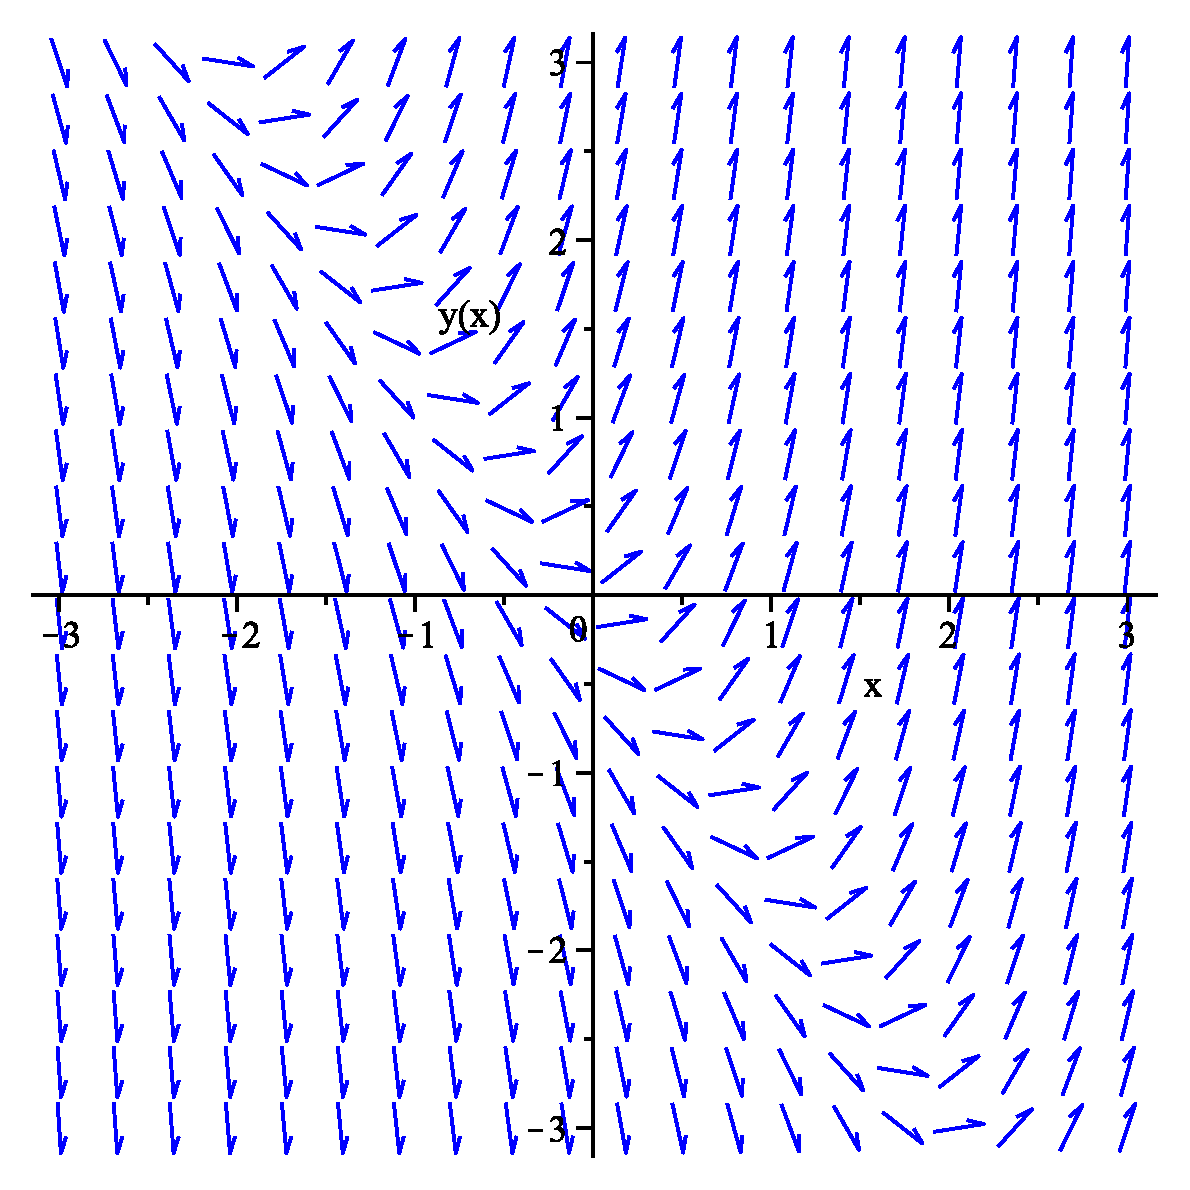
\includegraphics[width=3in]{slopefield1.eps}
\end{center}

The vectors indicate the tangent lines to graphs of solutions curves.  For example, if a solution $y(x)$ of this ODE has a graph that passes through the point $(0,1)$, then the slope of that curve will be $1$ at that point, because $y'=3(1)+(0)=3$, according to the differential equation $y'=3y+x$.  We will be able to verify this fact analytically once we know how to write down an explicit solution for this initial value problem: $y=-\frac{1}{9}-\frac{x}{3}+\frac{10}{9}e^{3x}$.  Indeed, we see that $y'=-\frac{1}{9}+\frac{10}{3}e^{3x}$, and at $x=0$ we get $y'=3$.  The following plot shows the graph of this solution $y(x)$ superimposed on the slope field.

\begin{center}
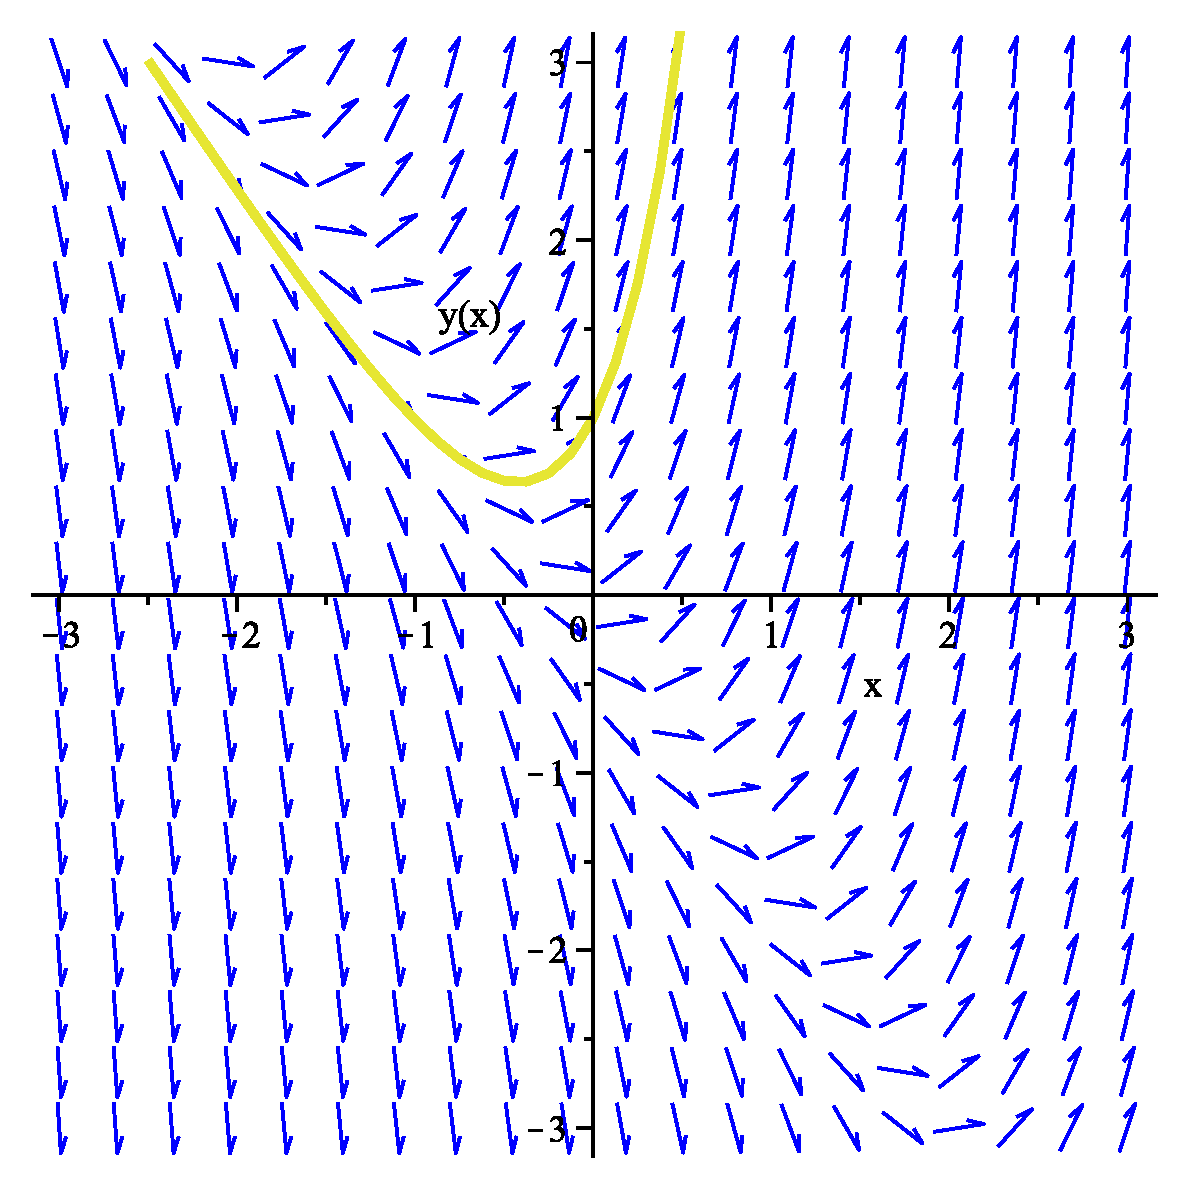
\includegraphics[width=3in]{slopefield2.eps} 
\end{center}

With a slope field, we can explore the behaviour of solutions {\it without} having an explicit formula for the solution.  For example, we could see from the slope field above that if a solution passed through the point $(0,1)$, then as $x$ increases so will $y$.  We can even guess that $\lim_{x \rightarrow \infty} y(x)=\infty$ (provided that the interval of definition of $y$ extends all the way to infinity).

In contrast, imagine a solution of $y'=3y+x, \ y(0)=-1$ is graphed on top of the slope field.  Then the solution will be decreasing at first as x increases. The plot below shows a curve that passes through $(0,-1)$ and whose tangent lines at each point are parallel to the slope field at each point.  This graph is our sketch of a solution to the initial value problem.

\begin{center}
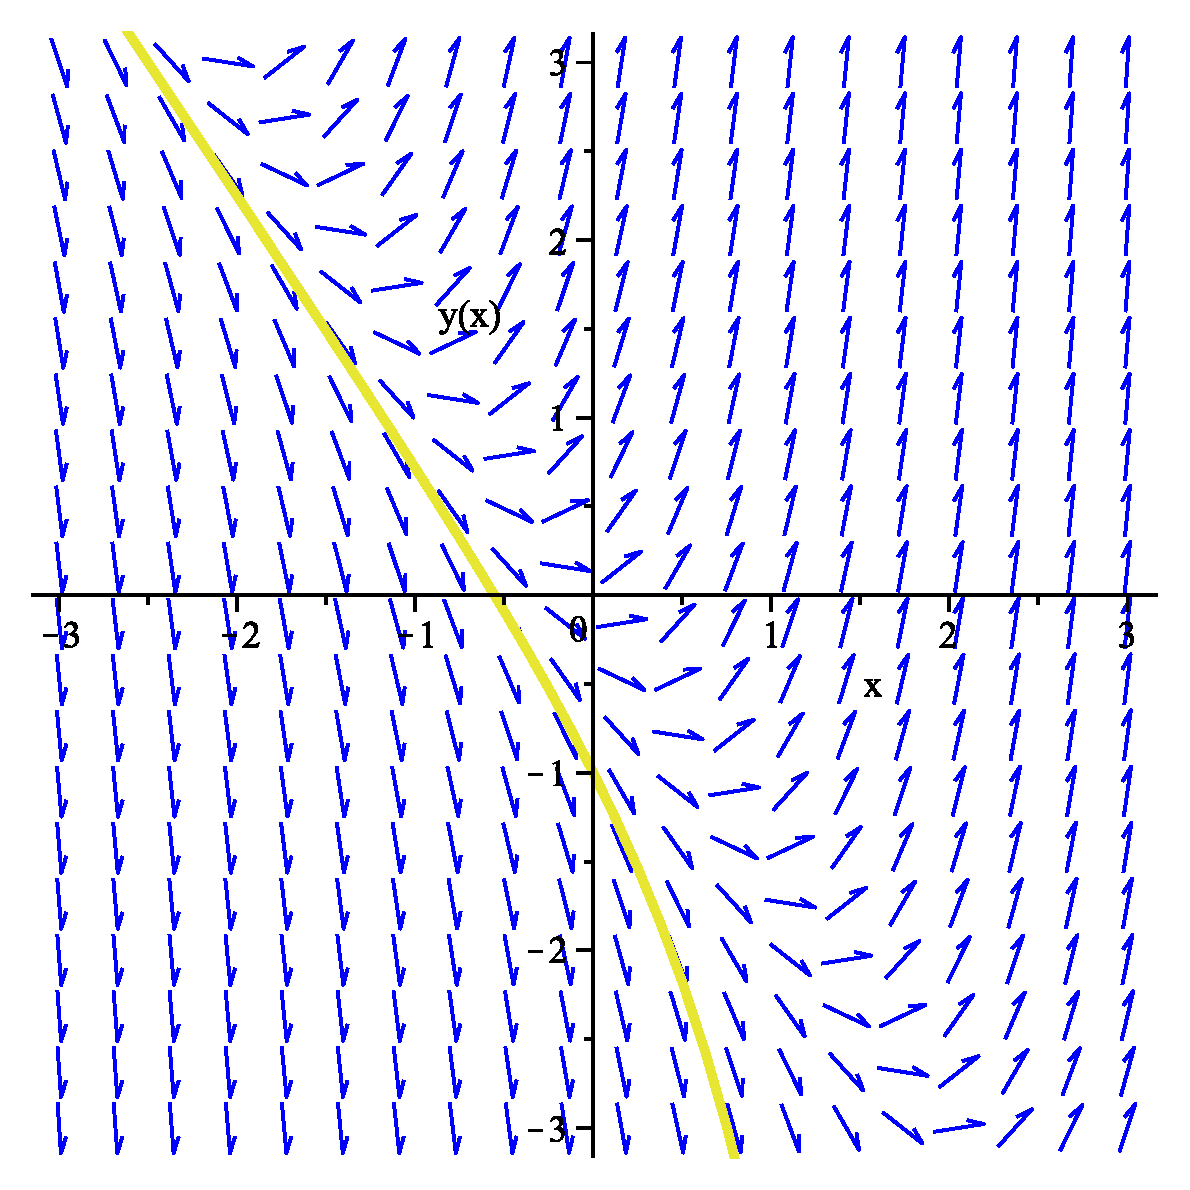
\includegraphics[width=3in]{slopefield3.eps}
\end{center}

Slope fields can be generated by hand, but it is usually much more efficient to use a computer program to generate them.  

\exercise Generate a slope field for $y'=y(y-2)$.  Then sketch several solution curves on the plot: one for each of the following initial conditions: $y(0)=-1$, $y(0)=0$, $y(0)=1$, and $y(0)=2$.  In each case, use the behaviour you see on the slope field to predict the value of $\lim_{x \rightarrow \infty} y(x)$. 

\exercise Use a slope field to predict the behaviour of $\lim_{x \rightarrow \infty} y(x)$, where $y$ is a solution of $y'=y+4$.  Explain how this limit depend on the initial value $y(0)$.

\exercise Use a slope field to predict the behaviour of $\lim_{x \rightarrow \infty} y(t)$ where $y$ is a solution of $\dot{y}=y-t$, $y(0)=0$

\exercise Use a slope field to predict the behaviour of solutions to $y'=y^2$.  Then confirm your prediction by finding a formula for the solution of the initial value problem $y'=y^2, \ y(0)=y_0$.  {\it (Hint: Use separation of variables.)}

\bigskip
Slope fields also provide us with some intuition regarding the existence and uniqueness of solutions.  It seems like, given a slope field representing a differential equation of the form $\frac{dy}{dx}=f(x,y)$ and a point in the plane $(x_0,y_0)$ representing the initial condition, we ought to be able to find a curve through that point that follows the slope field.  This suggests that initial value problems of the form $y'=f(x,y), \ y(x_0)=y_0$ ought to have solutions (at least in some interval containing $x_0$).  Indeed, if $f(x,y)$ is a nice function, then this is the case, and we will give a rigorous proof of this fact in a later chapter.  

Notice that the easiest slope fields to plot, if we need to do so by hand, are the ones where the right side of the differential equation depends on only one variable, such as $\frac{dy}{dx}=f(y)$, because all the direction vectors along a horizontal line have the same slope.  These have a special name: we say that a differential equation of the form $y'=f(y)$ is {\bf autonomous}.

Incidentally, equations of the form $y'=g(x)$ also have slope fields that are easy to plot, since the direction vectors along any vertical line have the same slope; however, these equations are not of as much interest to us in this course since they were studied extensively in calculus -- a solution of $y'=g(x)$ is just an antiderivative of the function $g$.

Next, we turn our attention to another graphical approach for understanding solutions of differential equations that is specifically applicable to autonomous equations.

\example Suppose the velocity $v(t)$ (in meters per second) of a falling object that encounters air resistance is modelled by the differential equation
\[ \dot{v} = 9.8-Kv\]
where $K>0$ is a constant.  The idea here is that air resistance is a force that is proportional to the speed of the object, and so the constant of proportionality K here depends on both the speed and the mass of the falling object; the $9.8$ account for the acceleration due to gravity, and by selecting a positive quantity here, we have implicity assume that positive velocities correspond to {\it downward} motion.  

Let us graph $\dot{v}$ as a function of $v$:

\begin{center}
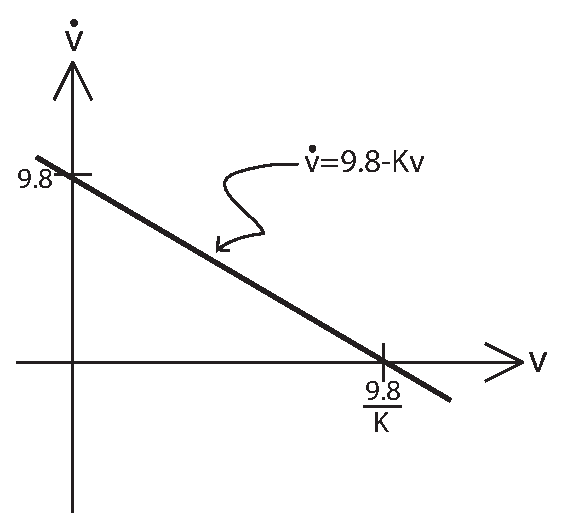
\includegraphics[width=4in]{phaseline1.eps}
\end{center}

The graph intersects the $v$-axis at $v=\frac{9.8}{K}$.  According to this graph, whenever the velocity is less than $\frac{9.8}{K}$, $\dot{v}$ will be positive, and therefore the object will continue to increase its velocity.  Similarly, if the velocity were to start out above $\frac{9.8}{K}$, then $\dot{v}$ will be negative, and therefore the velocity will decrease.  In both cases, the velocity will head toward the value $v=\frac{9.8}{K} \frac{m}{s}$.  And if the initial velocity is exactly $\frac{9.8}{K} \ \frac{m}{s}$, then $\dot{v}=0$ so the velocity will remain constant. We use arrows on a number line to illustrate the behaviour of the solution as follows:

\begin{center}
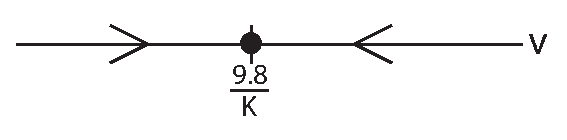
\includegraphics[width=4in]{phaseline2.eps}
\end{center}

This figure is called the {\bf phase line} for the differential equation: it indicates the constant solutions of the equation with dots (in this case, $v=\frac{9.8}{K}$ is the only constant solution), and it uses arrow to indicate the {\bf long-term behaviour} of solutions with other initial conditions.

In this application, the constant solution is called the {\bf terminal velocity} of the falling object -- it is the limiting value of the velocity as $t$ increases:
\[ \lim_{t \rightarrow \infty} v(t) = \frac{9.8}{K} \ \frac{m}{s}.\]
\qed

\exercise Suppose that an object is known from observations to have a terminal velocity of $196 \frac{m}{s}$.  Write down an initial-value problem for the velocity of this object if the initial velocity is $0 \frac{m}{s}$.

\exercise A tank contains a changing mixture of pure water and brine (salt water solution).  The differential equation that models the quantity of salt in the tank after $t$ minutes have passed is
\[ \dot{S} = 8-\frac{4S}{25} \ \frac{grams}{min}\]
where $S(t)$ is measured in grams.  Use a phase line analysis to determine the long-term behaviour, $\lim_{t \rightarrow \infty} S(t)$.




%% Cut below here for the book form.

\begin{center} {\LARGE Problems} \end{center}

\setcounter{problem}{1}

\problem Use a phase line analysis to determine the long-term behaviour of solutions to the differential equation 
\[ \dot{y} = \sin(y).\]
How does the behaviour depend on the initial value $y(0)$?

\problem Perform a phase line analysis for the logistic differential equation, $\dot{P}=kP(M-P)$.

\problem Find a differential equation $\dot{y}=f(y)$ which is consistent with the phase line shown below (there is more than one correct answer):

\begin{center}
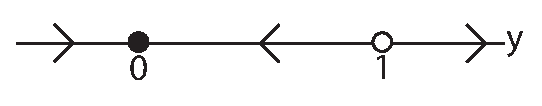
\includegraphics[width=4in]{phaseline3.eps}
\end{center} 






\end{document} % GRAPHICAL METHODS

\documentclass[12pt,letterpaper,twoside]{amsart}
\usepackage[latin1]{inputenc}
\usepackage{amsmath}
\usepackage{amsfonts}
\usepackage{graphicx}
\usepackage{amssymb}
\usepackage{multicol}
\usepackage{ulem}
\newcounter{example}
\newcounter{exercise}
\newcounter{problem}
\newtheorem{theorem}{Theorem}
\newcommand{\example}{\bigskip \noindent {\large {\sc Example \arabic{example}:}} \addtocounter{example}{1}}
\newcommand{\exercise}{\bigskip \noindent {\large {\sc Exercise \arabic{exercise}:}} \addtocounter{exercise}{1}}
\newcommand{\problem}{\bigskip \noindent {\large {\sc Problem \arabic{problem}:}} \addtocounter{problem}{1}}
\newcommand{\tech}{\marginpar{\vskip 10mm \begin{center}\includegraphics[width=0.25in]{calculatorimagesmall.eps} \end{center}}}
\newcommand{\solution}{\medskip \noindent {\bf Solution: }}
\newcommand{\R}{\mathbb{R}}





\begin{document}

\sffamily

%%%%  switch the commenting on this line and the next \chapter{Introduction}
\begin{center} {\LARGE Numerical Methods} \end{center}

\setcounter{example}{1}
\setcounter{exercise}{1}

In this chapter, we wil discuss a method for finding approximate values of solutions to ODE even when it is not possible to find formulas for solutions analytically.

The first example below will illustrate the basic idea of our approach, and the second example will demonstrate the fully developed idea.

\example Consider the initial value problem
\[ \left\{ \begin{matrix} y'=y^2-x \\ y(0)=1 \end{matrix} \right.\]
Suppose we want to know the value of $y(1)$, but we are unable to calculate an exact solution for the ODE.  We can still find an approximate solution as follows.

If $y(x)$ is the solution, then the initial condition implies that $y(0)=1$, and if we insert $x=0$ and $y=1$ into the differential equation, that tells us that $y'(0)=(y(0))^2-(0)=(1)^2-0=1$.  Therefore the tangent line approximation to $y(x)$ at the point $(0,1)$ is 
\[ y(x) \approx x+1.\]
Therefore we can deduce that $y(1)\approx 2$.
\qed

This picture illustrates the solution curve and the tangent line in the first example:
\begin{center}
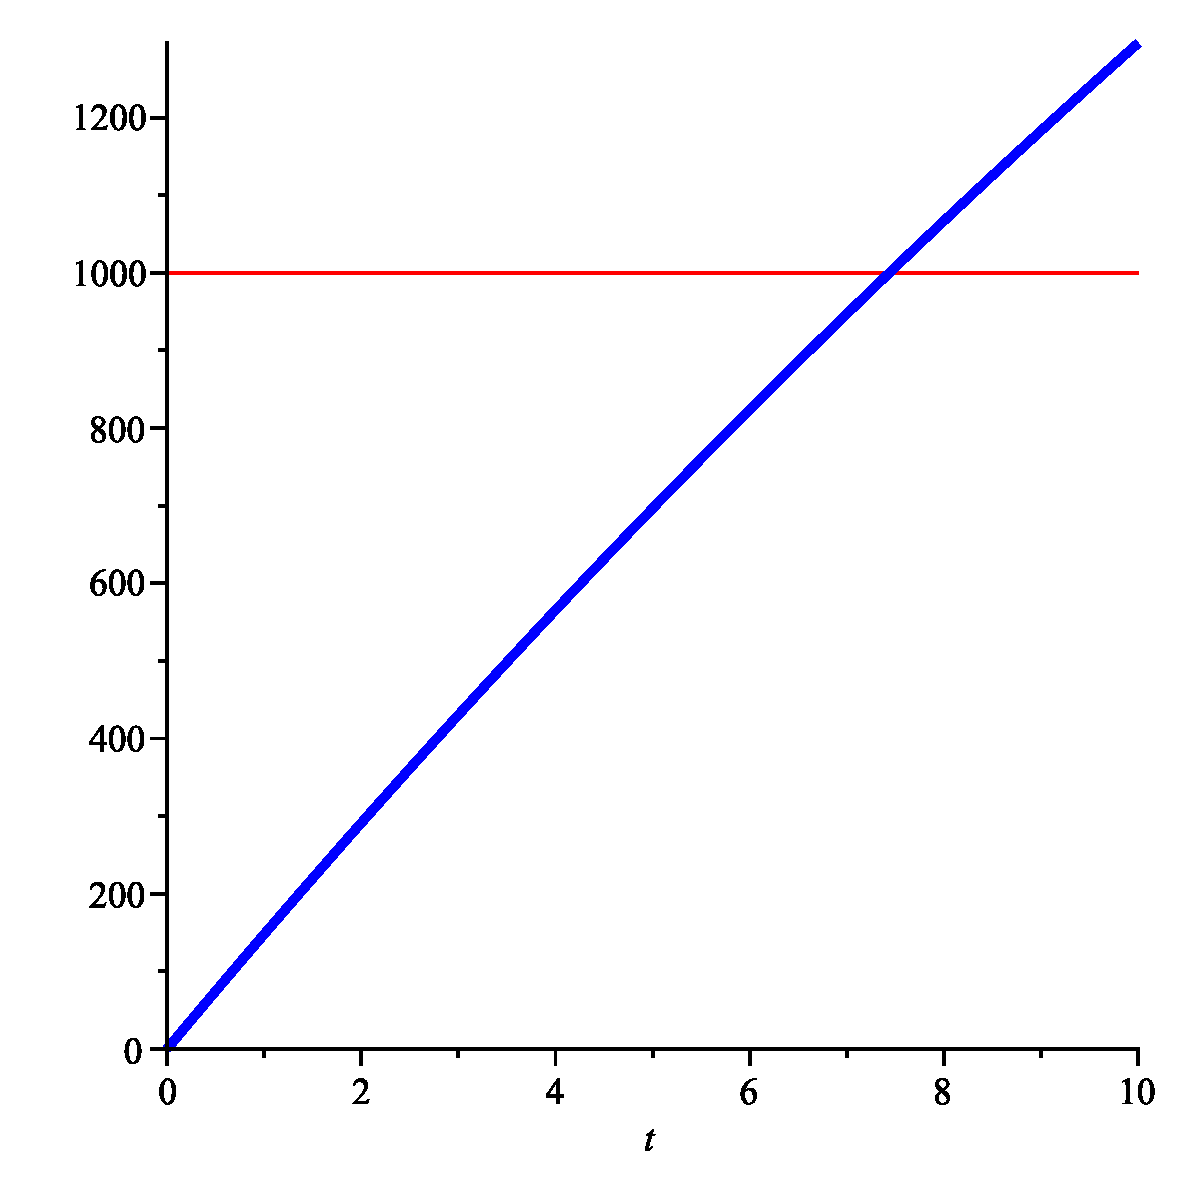
\includegraphics[width=3in]{example1.eps}
\end{center}
The idea was that, because we know the slope of the solution curve at the initial point $(0,1)$, we can use that to project what happens as $x$ increases.  However, it is not hard to see that the linear approximation is only good for small values of $x$ -- the actual solution curve grows quickly as $x$ increases, and the difference between the curve and the tangent line will only worsen away from the initial point.

One way to compensate for this is to use a different type of approximation -- a piecewise linear one.

Instead of following the tangent line all the way to the point where $x=1$, let's just follow it until $x=0.5$; then, at that point, we'll recompute the slope based on the differential equation.  According to the tangent line approximation, when $x=0.5$, we get $y \approx 1.5$; inserting this into the differential equation gives us $y' \approx (1.5)^2-(0.5)=1.75.$  This becomes the slope for the segment from $x=0.5$ to $x=1$:
\begin{center}
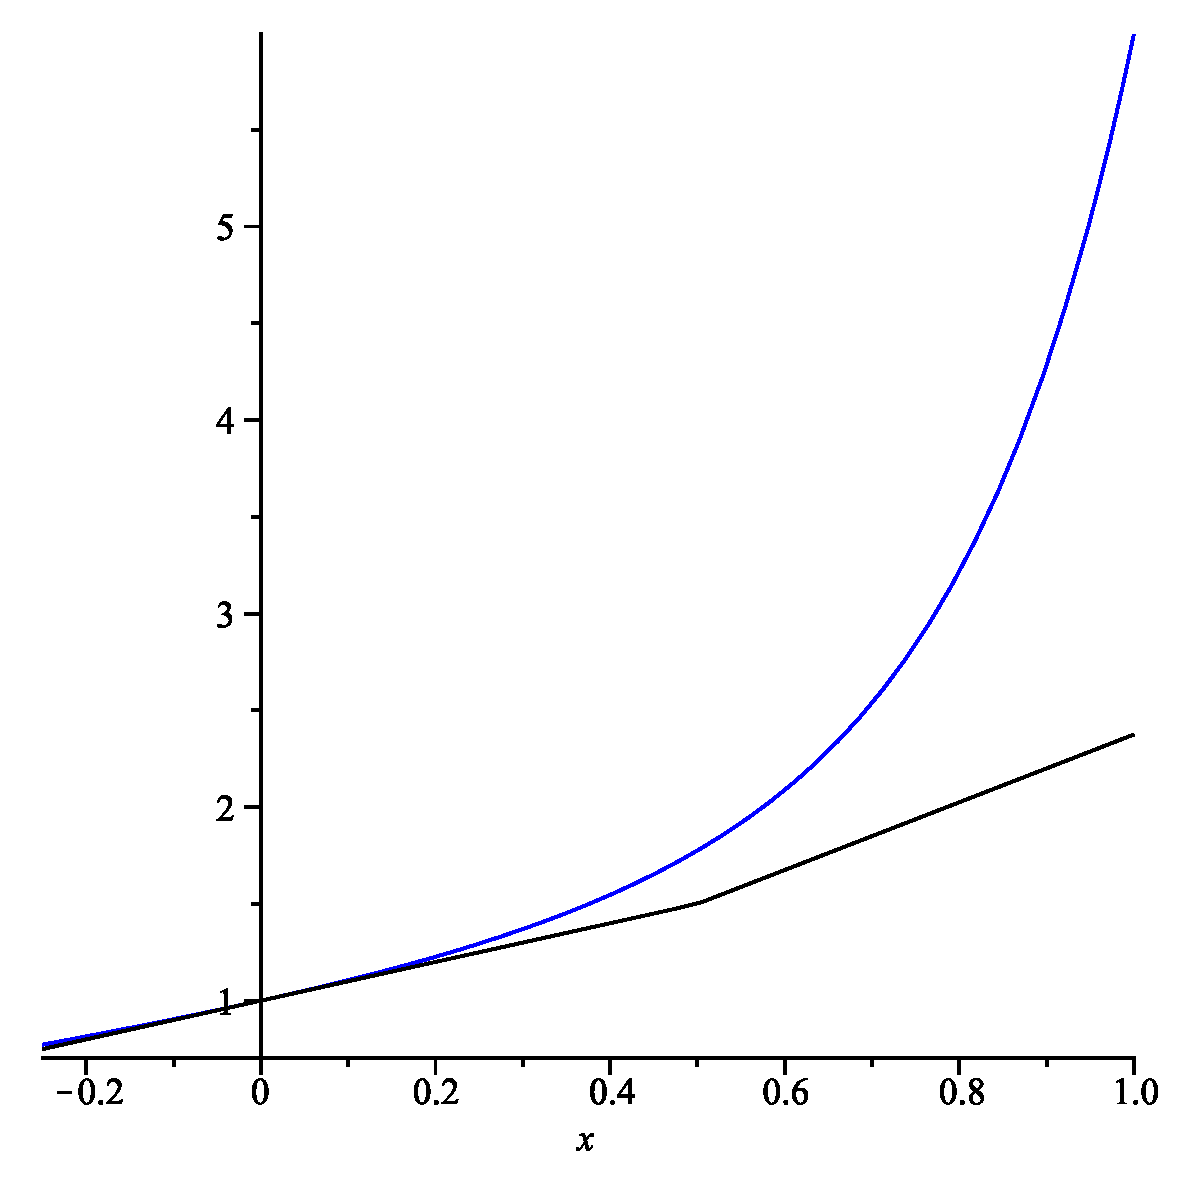
\includegraphics[width=3in]{example2.eps}
\end{center}
Based on this, we estimate that $y(1) \approx 1.5+0.5((1.5)^2-0.5))=2.375$.  Now our approach for finding an approximate solution has taken shape: by using a finer subdivision of intervals, we can obtain a better approximation for the value of $y(1)$.  The following graph shows how dividing the interval $[0,1]$ into 4 subintervals gives an even better approximation:





%% Cut below here for the book form.

\begin{center} {\LARGE Problems} \end{center}

\setcounter{problem}{1}

\problem Consider the following initial value problem: $y'=y, \ y(0)=y_0$.  {\bf (a)} Use Euler's method to find an approximate value for $y(x)$ by dividing the interval $[0,x]$ into $N$ subintervals of equal width.  (That is to say, you will use $\Delta x = \frac{x}{N}$.  {\it (Hint: Verify that $y_i=y_0(1+\Delta x)^i$.)}  {\bf (b)} Take a limit of the result in (a) as $N \rightarrow \infty$ to get the exact value of $y(x)$.






\end{document} % NUMERICAL METHODS

\documentclass[12pt,letterpaper,twoside]{amsart}
\usepackage[latin1]{inputenc}
\usepackage{amsmath}
\usepackage{amsfonts}
\usepackage{graphicx}
\usepackage{amssymb}
\usepackage{multicol}
\usepackage{ulem}
\newcounter{example}
\newcounter{exercise}
\newcounter{problem}
\newcommand{\example}{\bigskip \noindent {\large {\sc Example \arabic{example}:}} \addtocounter{example}{1}}
\newcommand{\exercise}{\bigskip \noindent {\large {\sc Exercise \arabic{exercise}:}} \addtocounter{exercise}{1}}
\newcommand{\problem}{\bigskip \noindent {\large {\sc Problem \arabic{problem}:}} \addtocounter{problem}{1}}
\newcommand{\tech}{\marginpar{\vskip 10mm \begin{center}\includegraphics[width=0.25in]{calculatorimagesmall.eps} \end{center}}}
\newcommand{\solution}{\medskip \noindent {\bf Solution: }}
\newcommand{\R}{\mathbb{R}}





\begin{document}

\sffamily

%%%%  switch the commenting on this line and the next \chapter{Introduction}
\begin{center} {\LARGE The Method of Integrating Factors} \end{center}

\setcounter{example}{1}
\setcounter{exercise}{1}

We say an ordinary differential equation of order 1 is linear if it can be written in the form:
\begin{equation} a(t)y'(t)+b(t)y(t)=f(t) \label{firstorderlinear} \end{equation}
In this chapter, we will explore a technique for analytically solving these differential equations and other equations that can be written in this form.

\example Solve the initial value problem $\frac{dy}{dx} = 3-4y, \ y(0)=1$.

First, let us rewrite the differential equation in the form:
\[ \frac{dy}{dx}+4y=3.\]
Next, mutiply both sides of the equation by $e^{4x}$ to obtain
\[ e^{4x} \frac{dy}{dx} + 4e^{4x} y = 3e^{4x}.\]
The point of this last step is that the left side of the equation is now the derivative of $e^{4x}y$:
\[ \frac{d}{dx}\left[ e^{4x} y \right] = 3e^{4x}.\]
If we anti-differentiate both sides with respect to $x$, we obtain
\[ e^{4x} y = \int 3e^{4x} \ dx = \frac{3}{4} e^{4x} + C.\]
Isolating $y$ gives us
\[ y = \frac{3}{4} + Ce^{-4x}.\]
The initial condition $y(0)=1$, implies that $C = \frac{1}{4}$.  Therefore the solution of the IVP is
\[ y=\frac{3}{4}+\frac{1}{4}e^{-4x}.\]
\qed

Multiplying by the expression $e^{4x}$ is what allowed us to recognize the left side of the equation as the derivative of an expression (which would have come from using the product rule), and that was what allowed us to simplify when we integrated both sides of the equation.  For that reason, the expression is referred to as an {\bf integrating factor}.

Any first-order linear differential equation written in standard form, 
\begin{equation} \frac{dy}{dx}+p(x)y=q(x),\label{standardfirstorderlinear} \end{equation}
is a candidate for this {\bf method of integrating factors}.  Once an equation is written in this form, we multiply both sides by the integrating factor $e^{\int p(x) dx}$:
\[ e^{\int p(x) dx} \frac{dy}{dx} + p(x) e^{\int p(x) dx} y = q(x) e^{\int p(x) dx}.\]
Now we can use the product rule to recognize the left side as a derivative:
\[ \frac{d}{dx} \left[ e^{\int p(x) dx} y \right] = q(x) e^{\int p(x) dx}.\]
Anti-differentiate both sides to get
\[ e^{\int p(x) dx} y = \int q(x) e^{\int p(x) dx} \ dx,\]
and then isolate y:
\[ y = e^{-\int p(x) dx } \int q(x) e^{\int p(x) dx} \ dx.\]

The reader should not try to memorize this formula.  Instead, think of this as a general process that can be applied to solve the differential equation: 
\begin{enumerate} 
\item Write the first-order linear equation in standard form;
\item Multiply by an appropriate integrating factor of the form $e^{\int p(x) dx}$;
\item Use the product rule to rewrite the left side as a derivative;
\item anti-differentiate both sides;
\item isolate $y$.
\end{enumerate}

Note that, in practice, any anti-derivative of $p(x)$ will suffice when you construct an integrating factor, so we may ignore the constant of integration when we find $e^{\int p(x) dx}$.

\exercise Solve the initial value problem $y' = y+e^x, \ y(0)=3$.

\exercise Solve the initial value problem $\dot{y} = xy+x, \ y(0)=1$.


\example Consider a 100-gallon tank that begins full of pure water.  Salt water solution containing 50 grams of salt per gallon is added to the tank at a rate of 2 gallons per minute.  Simultaneously, the solution in the tank is kept thoroughly mixed, and the tank drains at a rate of 3 gallons per minute.  Find the quantity of salt in the tank after 10 minutes.

Let us begin by writing a differential equation that describes the rate at which the quantity of salt in the tank is changing over time.  Let $S(t)$ represent the number of grams of salt in the tank after $t$ minutes.  Then
\[ \frac{dS}{dt} = \mbox{(rate in) - (rate out)},\]
where {\it rate in} refers to the rate at which salt is being added to the tank and {\it rate out} refers to the rate at which salt is leaving the tank.  Salt enters at a rate of 
\[\mbox{rate in} = \left( \frac{50 \ grams}{1 \ gallon}\right) \left( \frac{2 \ gallons}{1 \ minute}\right) = \frac{100 grams}{minute}.\]
The concentration of salt in the tank at any given instant is $\frac{S(t)}{V(t)}$, where $V(t)$ is the volume of liquid in the tank after $t$ minutes.  Because the liquid enters the tank at 2 gallons per minute but leaves at 3 gallons per minute, the volume is decreasing at 1 gallon per minute.  Therefore the volume will be $V(t) = 100-t$ gallons, so the concentration of salt in the tank is $\frac{S}{100-t} \frac{grams}{gallon}$.  Consequently, the rate at which salt is leaving the tank is described by:
\[ \mbox{rate out} = \left( \frac{S}{100-t} \frac{grams}{gallon}\right)  \left(\frac{2 gallons}{1 minute}\right) = \frac{2S}{100-t} \frac{grams}{minute}.\]
Hence
\[ \frac{dS}{dt} = 100 - \frac{2S}{100-t} \ \frac{grams}{minute}.\]
Also, the tank initially contains pure water, so $S(0)=0$.  Now we will solve this initial value problem for $S$.

Write the equation in the form
\begin{equation} \frac{dS}{dt} + \frac{2}{100-t} S = 100. \label{example2} \end{equation}
The integrating factor we need here is
\begin{align*} e^{\int \frac{2}{100-t} dt} 
& = e^{-2 \ln |100-t|} \\
& = e^{\ln (100-t)^{-2}} \\
& = \frac{1}{(100-t)^2}.
\end{align*}
Multiply both sides of the differential equation by this factor:
\[ \frac{1}{(100-t)^2}\frac{dS}{dt} + \frac{2}{(100-t)^3} S = \frac{100}{(100-t)^2}.\]
Reversing the product rule, we write this as
\[ \frac{d}{dt} \left[ \frac{1}{(100-t)^2} S \right] = \frac{100}{(100-t)^2},\]
and anti-differentiation leads us to
\begin{align*} \frac{1}{(100-t)^2} S 
& = \int \frac{100}{(100-t)^2} \ dt \\
& = \frac{100}{100-t}+C.
\end{align*}
Isolating $S$ gives us
\[ S = 100(100-t)+C(100-t)^2.\]
The initial condition $S(0)=0$ implies $C=-1$, so the solution of the IVP is
\[ S= 100(100-t)-(100-t)^2 \ \mbox{grams}.\]
Finally,  we calculate $S(10)$:
\[ S(10) = 100(90)-(90)^2=900.\]
This tells us that there will be 900 grams of salt in the tank after 10 minutes.
\qed

It is important to note that the solution in the above example only makes physical sense for $0 \leq t \leq 100$ (after that the model we constructed would predict a negative volume of liquid in the tank).

The next example will illustrate how we can sometimes solve a non-linear differential equation by converting it into a related linear equation.

\example Find a solution of the initial value problem $\dot{y}=\frac{y}{t}+y^2, \ y(1)=\frac{1}{2}$ defined for positive numbers $t$.

This differential equation is not separable, and it is not linear.  However, we can find a related linear differential equation in the following way: let $u = \frac{1}{y}$.  Then we have
\begin{align*}
\dot{u} 
& = -\frac{1}{y^2} \dot{y} \ \ \ \mbox{(by the chain rule)} \\
& = -\frac{1}{y^2} \left( \frac{y}{t}+y^2 \right) \ \ \ \mbox{(by the differential equation $y$ must satisfy)} \\
& = -\frac{1}{ty} -1 \\
& = -\frac{u}{t}-1 \ \ \ \mbox{(since $u=y^{-1}$)}.
\end{align*}
Now we have a differential equation that $u$ must satisfy: $\dot{u}=-\frac{u}{t}-1$.  If we can solve this differential equation to find $u$, then we can take the reciprocal of that solution to find a formula for $y$. Rewrite this as
\[ \dot{u} + \frac{1}{t} u = -1.\]
Multiply both sides by the integrating factor $e^{\int \frac{1}{t} dt} = e^{\ln |t|}=|t|=t$ (since we are only asked to consider positive values for $t$):
\[ t\dot{u} + u = -t.\]
Reversing the product rule on the left side gives us
\[ \frac{d}{dt} \left[ t u \right] = -t.\]
Integrate both sides with respect to $t$:
\[ t u = \int -t \ dt = -\frac{t^2}{2} + C.\]
Isolate $u$:
\[ u = -\frac{t}{2}+\frac{C}{t}\]
Because $u(1)=\frac{1}{y(1)}=\frac{1}{1/2}=2$, we obtain $C=\frac{5}{2}$.  This gives us the formula $u = -\frac{t}{2}+\frac{5}{2t}$, and taking the reciprocal yields
\[ y = \frac{1}{-\frac{t}{2} + \frac{5}{2t}},\]
or
\[ y = \frac{2t}{5-t^2}.\]
Observe that the interval of definition for this solution is $(-\sqrt{5},\infty)$.
\qed

The process above can be modified for any differential equation of the form
\[ \frac{dy}{dx}=p(x)y+y^N,\]
where $N$ is a positive integer.  These are called {\bf Bernoulli equations.}  For any such equation, the substitution $u=y^{1-N}$ leads to the differential equation
\[ \frac{du}{dx} = -Np(x)u-N,\]
which is a candidate for the method of integrating factors.  Again, the reader should not think of this as a formula to memorize but as a general procedure for Bernoulli equations:
\begin{enumerate}
\item Let $u=y^{1-N}$; use the chain rule and the differential equation for $y$ to find a differential equation for $u$;
\item solve for $u$ (be sure to modify the initial condition for $y$ appropriately);
\item use the solution for $u$ to obtain a formula for $y$.
\end{enumerate}

\exercise Solve the Bernoulli equation $y'=y+y^5$ subject to the initial condition $y(1)=3$.






%% Cut below here for the book form.

\begin{center} {\LARGE Problems} \end{center}

\setcounter{problem}{1}

\problem Find the general solution of the differential equation $a\dot{y}+by=c$, for any constant coefficients $a, \ b, \ c$, with $a \neq 0$.  {\it (Hint: You should consider the cases $b=0$ and $b \neq 0$ separately.)}

\problem A large tank begins with 50 gallons of water into which is dissolved 10 grams of salt.  Salt water solution with a concentration of 5 grams of salt per gallon is added to the tank at a rate of 4 gallons per minute.  Meanwhile, the solution in the tank is thoroughly mixed and drains at a rate of 2 gallons per minute.  How long will it take until there are 1000 grams of salt in the tank?  How much liquid will be in the tank at that instant?


\problem A large object is dropped from an airplane.  The velocity $v$, measured in meters per second, satisfies
\[ \dot{v} = 9.8 -Kv,\]
where $K>0$ is a constant.  If the object is falling at $100 \frac{m}{s}$ after 10 seconds, determine how fast it will be falling after 20 seconds.

\problem A large object is dropped from an airplane at an altitude of 3000 meters.  The velocity $v$, measured in meters per second, satisfies
\[ \dot{v} = 9.8 -Kv,\]
where $K>0$ is a constant.  If the object falls 200 meters in the first 10 seconds, estimate when the object will hit the ground.  {\it (You will encounter an algebraic equation that cannot be solved analytically.  Solve it numerically or graphically, but keep as many decimal places of accuracy as you can throughout the problem-solving process.)}



\problem Solve the logistic differential equation $\dot{P}=kP(K-P)$ by treating it as a Bernoulli equation and making a substitution.

\problem The idea of substitution has application beyond Bernoulli equations.  For example, any differential equation of the form $y'=f(ax+by+c)$ can be transformed into a separable differential equation by means of the substitution $u=ax+by+c$.  Use this idea to solve the initial value problem:
\[ y'=(x+2y)^2, \ \ \ y(0)=1.\]

\problem Solve the initial value problem $y'=\sin^2(x-y), \ y(0)=1$.





\end{document} % FIRST-ORDER LINEAR EQUATIONS

\input{5-seriessolutions/taylorsolutions.chapter} % Taylor Series Solutions

\newpage
\thispagestyle{empty}

\color{white}
\section*{Focus on Modeling: Pendulums}
\normalcolor
\vspace{-24pt}
\begin{center}
\psframebox[style=fombox]{\begin{minipage}{6in}
\begin{center}
FOCUS ON MODELING

{\huge Pendulums}
\end{center}

\hspace{0.125in}
Attach a mass to the end of a stiff rod that is allowed to swing from a fixed point, and you have a pendulum.  Historically, pendulums have been used as accurate timekeeping pieces and accelerometers.  Let's analyze the behavior of a pendulum by finding a differential equation governing the rate of change of the angle $\theta$ between the rod and the vertical.  In our model, we will use a massless rod of length $L$, with a mass $m$ attached to the end.

\begin{center}
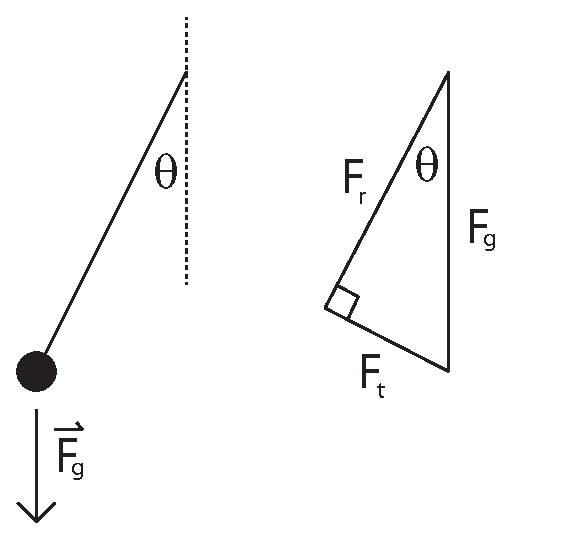
\includegraphics[width=3in]{FOM-pendulum/pendulum1.eps}
\end{center}

\hspace{0.125in}
The only external force acting on our pendulum is gravity, denoted by $\vec{F}_g$, which points downward with magnitude $mg$.  Let us decompose this vector into a sum of two vectors: one that is parallel to the rod, $\vec{F}_r$ ($r$ for `radial'); then the other vector, which we denote by $\vec{F}_t$, must be tangential to the path of the swinging mass.  For a given value of $\theta$, this decomposition is unique.  Trigonometric considerations tell us that 
\[ |\vec{F}_r| = |\vec{F}_g|\cos(\theta) \ \ \ \mbox{and} \ \ \ |\vec{F}_t | = |\vec{F}_g| \sin(\theta)|.\]
The tangential force $\vec{F}_t$ causes an acceleration of the mass along the circular path centered at the pendulum's fixed point.  We know from precalculus that the linear velocity of the mass is equal to the radius of the circle multiplied by the angular velocity, i.e., $L\dot{\theta}$.  Differentiating this expression gives us the acceleration, $L\ddot{\theta}$.  Newton's second law then tells us that the tangential force equal the mass times the acceleration:
\[ mL \ddot{\theta} = -mg\sin(\theta).\]
\end{minipage}
}
\end{center}

\newpage
\begin{center}
\psframebox[style=fombox]{\begin{minipage}{6in}
\hspace{0.125in}
Notice the negative sign on the right side of the equation: it is there because the direction of the acceleration will be opposite the direction of the displacement from $\theta=0$, since gravity will work to bring the mass back toward that position.  Dividing through by $m$ and rearranging terms gives us the differential equation
\[ \ddot{\theta}+\frac{g}{L}\sin(\theta)=0.\]

\hspace{0.125in}
There were three important assumptions made in deriving this model:
\begin{enumerate}
\item the rod remains taught and straight;
\item the pendulum moves in only two dimensions; and
\item the motion is not subject to resistance or friction.
\end{enumerate}
Even with these simplifications, the resulting differential equation is not simple to solve.  It can be analyzed using numerical or Taylor methods.  But in order to obtain analytic solutions, we usually make one more assumption: {\it the angle $\theta$ remains small.}  The point of this assumption is that, when $\theta$ is small, $\sin(\theta)\approx \theta$ (provided $\theta$ is measured in radians) which can be seen by neglecting the non-linear terms in the power series representation of sine: $\sin(\theta) = \sum_{n=0}^\infty \frac{(-1)^n \theta^{(2n+1)}}{(2n+1)!} = \theta - \frac{\theta^3}{3!}+\frac{\theta^5}{5!}- \cdots.$  Replacing $\sin(\theta)$ with $\theta$ gives us the simpler, approximate differential equation:
\[ \ddot{\theta} + \frac{g}{L}\theta=0.\]
This second-order linear differential equation can be solved analytically using the methods we will discuss in Chapter 7.

\end{minipage}
}
\end{center}

 % FOCUS ON MODELING: PENDULUM

\documentclass[12pt,letterpaper,twoside]{amsart}
\usepackage[latin1]{inputenc}
\usepackage{amsmath}
\usepackage{amsfonts}
\usepackage{graphicx}
\usepackage{amssymb}
\usepackage{multicol}
\usepackage{ulem}
\newcounter{example}
\newcounter{exercise}
\newcounter{problem}
\newtheorem{theorem}{Theorem}
\renewcommand{\proof}{{\bf Proof:}}
\newcommand{\example}{\bigskip \noindent {\large {\sc Example \arabic{example}:}} \addtocounter{example}{1}}
\newcommand{\exercise}{\bigskip \noindent {\large {\sc Exercise \arabic{exercise}:}} \addtocounter{exercise}{1}}
\newcommand{\problem}{\bigskip \noindent {\large {\sc Problem \arabic{problem}:}} \addtocounter{problem}{1}}
\newcommand{\tech}{\marginpar{\vskip 10mm \begin{center}\includegraphics[width=0.25in]{calculatorimagesmall.eps} \end{center}}}
\newcommand{\solution}{\medskip \noindent {\bf Solution: }}
\newcommand{\R}{\mathbb{R}}





\begin{document}

\sffamily

%%%%  switch the commenting on this line and the next \chapter{Introduction}
\begin{center} {\LARGE Existence and Uniqueness} \end{center}

\setcounter{example}{1}
\setcounter{exercise}{1}

Previously, we investigated the behaviour of solutions to various ODE.  The whole time, we assumed that there {\it were} solutions to the given equations.  Later, we will find approximate values for solutions of IVP using numerical methods which also assume that a solution exists.  But that assumption really requires proof if we are going to trust any of the conclusions we draw from the geometric approaches we took or the numerical methods we will employ later.  

The next theorem is the main result of this chapter.

\begin{theorem} Suppose that $f(y)$ and $f'(y)$ are defined and continuous on an open interval $(a,b)$ which contains $y_0$.  Then three is an open interval $I$ containing $x_0$ such that the initial value problem 
\[ \frac{dy}{dx}=f(y), \ \ \ y(x_0)=y_0\]
has a unique solution $y(x)$ defined on $I$.
\end{theorem}

We will prove this result in several stages, starting with the uniqueness part.  When we say that a solution to an IVP is unique on an interval $I$, we mean that if $y$ and $z$ are both functions that solve the IVP on $I$, then $y(t)=z(t)$ for all $t \in I$.  As the reader will find in the problems at the end of this chapter, uniqueness isn't always guaranteed.  But it is guaranteed (at least {\it near} $x_0$) when $f$ and $f'$ are both continuous.

The central idea in the uniqueness proof is a procedure called Picard iteration.  (This technique can also be used to prove existence, and this approach will be outlined in the problem set.)  Suppose that $y$ is a function defined on an interval $I$.  A {\bf Picard iterate} of $y$ is another function, $\tilde{y}$, defined according to the following formula:
\[ \tilde{y}(x) = y_0 + \int_{x_0}^x f(y(s)) \ ds\]

\exercise Suppose that $x_0=0$, $y_0=2$, $f(y)=y^2$ and $y(x)=x$.  Prove that $\tilde{y}(x)=2+\frac{s^3}{3}$.

\exercise Let $x_0=0$, $y_0=0$ and $f(y)=e^y$.  Find the Picard iterate of the function $y(x)=2x$.

\exercise Prove that $y(x)$ solves the initial value problem 
\[ \frac{dy}{dx}=f(y), \ \ \ y(0)=y_0\]
if and only if $\tilde{y}=y$.  {\it (Hint: Recall the Fundamental Theorem of Calculus.)}

The last exercise reveals the relationship between Picard iteration and initial value problems.  It allows us to recast the differential equation as an {\bf integral equation}: finding a solution $y(x)$ of the equation
\[ y(x)=y_0+\int_{x_0}^x f(y(s)) \ ds \]
is equivalent to finding a solution of the IVP $\frac{dy}{dx}=f(y), \ y(x_0)=y_0$.  The process below will illustrate how we go about verifying that the integral equation has a solution.

We need to define one more item of notation before we can proceed.  For a bounded function $f$ defined on an interval $I$, define
\[ \parallel f \parallel_I = \min \left\{ a; |f(x)|\leq a \mbox{ for all } x \in I \right\}.\]
This quantity is called the {\bf uniform norm} of $f$ on $I$, or just the {\bf norm} of $f$ for short.  Notice that if $|f|$ attains a maximum value on $I$, then $\parallel f \parallel_I = \max_{x \in I} |f(x)|$.

\exercise Let $f(x)=x^2-x$ on the interval $I=[0,1]$.  Prove that $\parallel f \parallel_I = \frac{1}{4}$.

\exercise Prove that if $\parallel f-g \parallel_I=0$, then $f(x)=g(x)$ for all $x \in I$.

The last exercise shows us how we can use the norm to identify when two functions are equal on a domain $I$: they are equal if the norm of their difference is zero.

\begin{theorem} Suppose that $|f'(y)| \leq K$, where $K \geq 0$ is some constant.  Then if the endpoints of the interval $I$ are $a$ and $b$, 
\[ \parallel \tilde{y} -\tilde{x} \parallel_I \leq K |b-a| \parallel y-z \parallel_I.\]
\label{contraction}
\end{theorem}

Notice that this theorem does not require that the interval $I$ be either open or closed.  $I$ may contain either endpoint $a$ or $b$, or both, or neither.

\proof 
For any $x \in I$ with $x \geq x_0$, we have
\begin{align*}
|\tilde{y}(x)-\tilde{z}(y)|
& = \left| y_0 + \int_{x_0}^x f(y(s)) \ ds - y_0 - \int_{x_0}^x f(z(s)) \ ds \right| \\
& = \left| \int_{x_0}^x (f(y(s)) - f(z(s))) \ ds \right| \\
& \leq \int_{x_0}^x |f(y(s))-f(z(s))| \ ds \\
& \leq \int_{x_0}^x K |y(s)-z(s)| \ ds \\
& \leq \int_{x_0}^x K \parallel y - z \parallel_I \ ds \\
& = K |x-x_0| \parallel y-z \parallel_I \\
& \leq K|b-a|\parallel y-z \parallel_I
\end{align*}
A small change to the calculation above shows that the same is true for $x \leq x_0$.  Since this inequality is true for all $x \in I$, it follows that 
\[\parallel \tilde{y}-\tilde{z} \parallel_I \leq K|b-a| \parallel y-z \parallel_I.\]
\qed

\exercise Modify the calculation in the proof above to deal with the case $x \leq x_0$.

\begin{theorem} Suppose that $f$ and $f'$ are defined and continuous on an open interval $(a,b)$ containing $y_0$.  Also suppose that  $|f'|<K$ on $(a,b)$, and $|b-a| < \frac{1}{K}$.  Then if $y_1$ and $y_2$ are both bounded functions that solve the IVP
\[ \frac{dy}{dx}= f(y), \ \ \ y(x_0)=y_0 \]
on the interval $I$, it must be true that $y_1(x)=y_2(x)$ for all $x \in I$.
\end{theorem}

\proof 
Let $L=K|b-a|$.  Then under the assumptions made here, we see that $L<1$.  Therefore we know that $\parallel \tilde{y_1} - \tilde{y_2} \parallel_I \leq L \parallel y_2 - y_1 \parallel_I.$  On the other hand, Ibecause $y_1$ and $y_2$ satisfy the IVP, it must be true that $\tilde{y_1}=y_1$ and $\tilde{y_2}=y_2$.  Putting these two facts together yields the inequality
\[ \parallel y_2-y_1 \parallel_I \leq L \parallel y_2-y_1 \parallel_I,\]
which can only be true if $\parallel y_2-y_1 \parallel_I = 0$ because we know $L < 1$.  (If this norm is not zero, divide both sides of the inequality by it to obtain $1 \leq L$, which would be a contradiction.)

Consequently, $y_2=y_1$ on $I$.
\qed

\begin{theorem} 
Suppose $f$ and $f'$ are defined on an interval $J$ containing $y_0$, and both functions are continuous on $J$.  Then there is an interval $I$ containing $x_0$ such that, if $y_2$ and $y_1$ are both solutions of 
\[ \frac{dy}{dx}=f(y), \ \ \ y(x_0)=y_0\]
on $I$, then $y_1=y_2$.
\end{theorem}
Another way to phrase the result of this theorem is that solutions of the IVP are unique in a neighborhood of $x_0$.

\proof
Because $f'$ is continuous at $y_0$, there is an open subinterval $\hat{J}$ of $J$ containing $y_0$ on which $f'$ is bounded.  Let 
\[K=\max_{z \in \hat{J}} |f'(z)|.\]
Let $a$ and $b$ denote the endpoints of $\hat{J}$, and define
\[ D=\min \{ |b-y_0|,|a-y_0| \},\]
so that $D$ is the minimum distance of $y_0$ from the endpoints of $\hat{J}$.  Define
\[ I = \left( x_0-\frac{D}{K}, x_0+\frac{D}{K} \right) .\]
Suppose that $y_1$ and $y_2$ are both solutions of the IVP on $I$.  For each $x \in I$,
\[ y_1(x)-y_0 = y_1(x)-y_1(x_0)=y_1'(x^*)(x-x_0)\]
for some $x^*$ between $x_0$ and $x$.  (This is a consequence of the mean value theorem.)  Thus $x^*$ is also contained in $I$, and therefore $|y'(x^*)|<K$.  Furthermore, $|x-x_0| \leq \frac{D}{K}$.  Consequently,
\[ |y_1(x)-y_0| = |y_1'(x^*)||x-x_0| < K \frac{D}{K}=D.\]
Since $|y_1(x)-y_0| < D$, it follows that $y_1(x) \in \hat{J}$ for all $x \in I$.  The same reasoning applies to $y_2$.  Now we can apply apply the previous theorem on the interval $I$ with the inequality $|f'|\leq K$ to obtain that $y_1=y_2$ on $I$.
\qed


With this last theorem, we have succeeded in proving the uniqueness part of Theorem 1.  It remains for us to prove that solutions do in fact exist.  It is possible to do this with Picard iteration -- in fact, for non-autonomous equations, that is exactly what we would need to do.  The idea is to define a sequence of functions $\{ y_i \}$, where each $y_i$ is the Picard iterate of $y_{i-1}$.  Then one proves that the sequence of functions $y_i$ converges to a function $y$ as $i \rightarrow \infty$, and then that this function $y$ is a solution.  This process is outlined in the problem set.

If we restrict our attention to autonomous equations here, we can use an alternative approach to proving existence which is somewhat easier.  The motivation for this proof is as follows.  If we were to try to solve the problem $\frac{dy}{dx}=f(y)$ using separation of variables, we'd end up with $\int \frac{1}{f(y)}\ dy = \int \ dx$, which is equivalent to the equation
\[ \int_{y_0}^y \frac{1}{f(s)} \ ds = x+C,\]
because, according to the Fundamental Theorem of Calculus, the left side is an anti-derivative of $\frac{1}{f(y)}$. 
Inserting the initial condition $x=x_0$ and $y=y_0$ yields $C=-x_0$, so we would have
\[ \int_{y_0}^y \frac{1}{f(s)} \ ds = x-x_0.\]
Finally, we would need to try to solve for $y$ in terms of $x$.  The following proof essentially verifies that the function $y(x)$ obtained in this way is indeed a solution of the IVP.


\begin{theorem} If $f$ is continuous on an open interval containing $y_0$, then there is a solution of the IVP
\[ \frac{dy}{dx}=f(y), \ \ \ y(x_0)=y_0\]
defined on an open interval containing $x_0$.
\end{theorem}

If $f(y_0)=0$, then the constant function $y(x)=y_0$ defined on $\mathbb{R}$ is a solution.  Now assume $f(y_0)>0$.  Because $f$ is continuous, there exists $\delta>0$ such that $f(s)>0$ for all $s \in [y_0-\delta, y_0+\delta]$.  Define
\[ G(t) = \int_{y_0}^t \frac{1}{f(s)} \ ds \ \ \ \mbox{for} t \in [y_0-\delta,y_0+\delta].\]
Notice that $G$ is continuous and because the integrand $\frac{1}{f(s)}>0$, $G$ is a strictly increasing function of $t$.  Therefore $G$ has a continuous inverse function $G^{-1}$ defined on the interval $[(G(y_0-\delta),G(y_0+\delta)]$.  Notice that this interval contains $0$ because $G(y_0)=0$. 

Let $I= (x_0+G(y_0-\delta),x_0+G(y_0+\delta)]$, and define 
\[ y = G^{-1} (x-x_0) \ \ \ \mbox{for} \ x \in I.\]
We claim that this formula defines a solution of the IVP.  First of all, 
\[ y(x_0)=G^{-1}(x_0-x_0)=G^{-1}(0)=y_0,\]
so the initial condition is satisfied.  Also, we can prove that the differential equation is satisfied by using implicit differentiation:
\begin{align*}
y&=G^{-1}(x-x_0)\\
G(y)&=x-x_0 \\
\frac{d}{dx}G(y)&=\frac{d}{dx}[x-x_0] \\
G'(y) \frac{dy}{dx}&= 1 \\
\frac{1}{f(y)}\frac{dy}{dx}&=1 \\
\frac{dy}{dx}&=f(y).
\end{align*}
The proof for the case when $f(y_0)<0$ is similar.
\qed

The following figures illustrate the domain and range we chose for the function $G$ in the proof above.  Here is a graph of $v=G(u)$:

\begin{center}
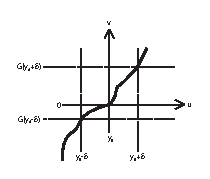
\includegraphics[width=3in]{existence1.eps}
\end{center}

And here is a graph of $u=G^{-1}(v)$:

\begin{center}
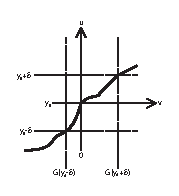
\includegraphics[width=3in]{existence2.eps}
\end{center}


%% Cut below here for the book form.

\begin{center} {\LARGE Problems} \end{center}

\setcounter{problem}{1}

\problem Verify that the functions
\[ y = \left\{ \begin{matrix} 0 & \mbox{for } x \leq a \\ \frac{1}{4}(x-a)^2 & \mbox{for } x > a \end{matrix} \right. \]
for $a>0$ all satisfy the IVP
\[ y'=\sqrt{y}, \ \ \ y(0)=0.\]
Therefore there are infinitely many solutions of the IVP.  Which hypothesis of Theorem 1 is not met in order that this might happen?  {\it (Hint: When you calculate the derivtive of $y$ to check the differential equation, make sure you use the limit definition of derivative at $x=a$.)}






\end{document} % EXISTENCE AND UNIQUENESS

\part{Second Order Equations}

\documentclass[12pt,letterpaper,twoside]{amsart}
\usepackage[latin1]{inputenc}
\usepackage{amsmath}
\usepackage{amsfonts}
\usepackage{graphicx}
\usepackage{amssymb}
\usepackage{multicol}
\usepackage{ulem}
\newcounter{example}
\newcounter{exercise}
\newcounter{problem}
\newtheorem{theorem}{Theorem}
\newcommand{\example}{\bigskip \noindent {\large {\sc Example \arabic{example}:}} \addtocounter{example}{1}}
\newcommand{\exercise}{\bigskip \noindent {\large {\sc Exercise \arabic{exercise}:}} \addtocounter{exercise}{1}}
\newcommand{\problem}{\bigskip \noindent {\large {\sc Problem \arabic{problem}:}} \addtocounter{problem}{1}}
\newcommand{\tech}{\marginpar{\vskip 10mm \begin{center}\includegraphics[width=0.25in]{calculatorimagesmall.eps} \end{center}}}
\newcommand{\solution}{\medskip \noindent {\bf Solution: }}
\newcommand{\R}{\mathbb{R}}





\begin{document}

\sffamily

%%%%  switch the commenting on this line and the next \chapter{Introduction}
\begin{center} {\LARGE Second Order Constant Coefficient ODE} \end{center}

\setcounter{example}{1}
\setcounter{exercise}{1}

We would next like to write down solutions for second-order constant coefficient linear ODE.  These have the form:
\[ a y''+by'+cy=f(x).\]
Here, the coefficients $a$, $b$ and $c$ are constant, and we assume that $a\neq 0$ so that the equation will indeed be second order.  We will first focus on homogeneous equations:
\[ ay''+by'+cy=0.\]
Let us seek some inspiration by studying the similar problem for first-order equations.

The general solution of the first order homogeneous constant-coefficient linear equation
\[ ay'+by=0, \ \ \ a \neq 0.\]
is
\[ y = Ce^{-bt/a},\]
which can be verified by the method of integrating factors.  If $b=0$, then the solution is just a constant function $y=C$.  Notice that if $y=Ae^{rt}$ satisfies the ODE $ay'+by=0$, then the constant $r$ satisfies the algebraic equation $ar+b=0$.  This will serve as our starting point for trying to understand second order equations.

\exercise Prove that if $y=Ae^{rx}$ satisfies the differential equation $ay''+by'+cy=0$, then $r$ is a solution of the algebraic equation $ar^2+br+c=0$.  

\medskip
The algebraic equation $ar^2+br+c=0$ is called the {\bf characteristic equation} for the ODE $ay''+by'+cy=0$.  The previous exercise indicates that there is a connection between the solutions of the ODE and the solutions of the corresponding characteristic equation.  The following exercise completes the description of that connection.

\exercise Prove that if $r$ is a root of $ar^2+br+c=0$, then for any constant coefficient $A$, the function $y=Ae^{rt}$ satisfies the differential equation $ay''+by'+cy=0$. {\it (Note that $r$ might equal zero.)}

\medskip
Also, because the ODE $ay''+by'+cy=0$ is linear in $(y,y',y'')$, we know that if $y_1$ and $y_2$ are both functions that satisfy the differential equation, then so does the sum $y=y_1+y_2$.  This and the results of the previous exercises demonstrate that the following is true:  If $r_1$ and $r_2$ are roots of the characteristic equation $ar^2+br+c=0$, then functions of the form $y=Ae^{r_1t}+Be^{r_2t}$ satisfy the ODE $ay''+by'+c=0$.

In fact:
\begin{center}
\fbox{
\begin{minipage}{3in}
If the characteristic equation for 
\[ ay''+by'+cy=0\]
has two distinct roots $r_1$ and $r_2$, then the formula 
\[ y=Ae^{r_1t}+Be^{r_2t}\] 
provides us with the {\bf general solution} on $\mathbb{R}$ of this differential equation.
\end{minipage}
}
\end{center}
By distinct, we mean that $r_1 \neq r_2$.  (The fact that it is indeed the {\it general solution} is explored in the problem set at the end of this chapter.)  We still need to investigate what to do if the characteristic equation has a repeated root (that is to say, if it is equivalent to the equation $a(r-r_1)^2=0$).  But first let us explore a few examples involving non-repeated roots.

\example Find the solution of the initial value problem $y''+5y'+6=0$, $y(0)=0$, $y'(0)=2$.

First we identify the characteristic equation for this ODE: $r^2+5r+6=0$.  Solving this algebraic equation gives us the solutions $r_1=-2$ and $r_2=-3$.  Therefore, the general solution of the ODE is
\[ y=Ae^{-2x}+Be^{-3x}.\]
If we substitute in the given initial conditions, we obtain the system of equations:
\[ 0=A+B, \ \ \ 2 = -2A-3B\]
Solving this system of equations lead to the values $A=2, B=-2$.  Consequently, the solution of this initial value problem is
\[ y = 2e^{-2t}-2e^{-3t}.\]
\qed




\exercise Solve the following initial value problems:
\begin{itemize}
\item $y''-y'+6=0, \ \ \ y(0)=2, \ \ \ y'(0)=0$
\item $2y''-5y'+2y=0, \ \ \ y(0)=1, \ \ \ y'(0)=2$
\end{itemize}

The process identified above even works when the solutions of the characteristic equation are complex numbers, though in that case it is often more convenient to write the solutions in a different form.

Recall that if a complex number is written in the form $\alpha + i \beta$, where $\alpha$ and $\beta$ are real, then $e^{\alpha+i\beta}=e^\alpha(\cos(\beta)+i\sin(\beta))$.  Also, if the characteristic equation has real coefficients but complex roots, the the roots must be complex conjugates of one another.  Therefore the general solution has the form:

\begin{align*} 
y & = A e^{(\alpha+i\beta)x}+Be^{(\alpha-i\beta)x} \\
& = Ae^{\alpha x}(\cos(\beta x)_i\sin(\beta x)) + Be^{\alpha x}(\cos(-\beta x)+i\sin(-\beta x) \\
& = Ae^{\alpha x}(\cos(\beta x)_i\sin(\beta x)) + Be^{\alpha x}(\cos(-\beta x)-i\sin(-\beta x) \\
& = (A+B)e^{\alpha x}\cos(\beta x)+(A-B)ie^{\alpha x}\sin(\beta x)
\end{align*}

If we introduce new coefficients $C$ and $D$ satisfying $C=A+B$ and $D=(A-B)i$, then we obtain the form
\[ y = Ce^{\alpha x}\cos(\beta x)+De^{\alpha x}\sin(\beta x).\]

This gives us:

\begin{center}
\fbox{
\begin{minipage}{3in}
If the characteristic equation $ar^2+br+c=0$ has complex roots of the form $r_1=\alpha+i\beta$ and $r_2=\alpha-i\beta$, then the general solution on $\mathbb{R}$ of the ODE $ay''+by'+cy=0$ can be written in the form
\[ y=Ce^{\alpha x}\cos(\beta x)+De^{\alpha x}\sin(\beta x).\]
\end{minipage}
}
\end{center}


\exercise Solve the following initial value problems.
\begin{itemize}
\item $y''+2y'+2y=0, \ \ \ y(0)=1, \ \ \ y'(0)=0$
\item $3\ddot{y}+5\dot{y} +2y=0, \ \ \ y(0)=2, \ \ \ y'(0)=0$.
\end{itemize}


Finally, we need to determine how to find a general solution to $ay''+by'+cy=0$ when the characteristic equation yields only one root, $r_1$.  In this case, we know that the expression $e^{r_1x}$ gives one solution of the ODE which is never zero.  We will use reduction or order to find the general solution.  Let $y$ be any solution of the ODE, and write $y=ue^{r_1x}$.

The product rule gives us $y'(x)=u'e^{r_1x}+r_1ue^{r_1x}$ and $y''(x)=u''e^{r_1x} + 2r_1u'e^{r_1x}+r_1^2ue^{r_1x}$.  Now we can substitute $ue^{r_1x}$ for $y(x)$ in the differential equation:

\begin{align*}
0 & = ay''+by'+cy \\
& = a(u''e^{r_1x} + 2r_1u'e^{r_1x}+r_1^2ue^{r_1x}) \\
& \ \ \ \ \ + b(u'e^{r_1x}+r_1ue^{r_1x}) + c(ue^{r_1x}) \\
& = au''e^{r_1x} + (2ar_1+b)u'e^{r_1x} +(ar_1^2+br_1+c)ue^{r_1x} \\
& = au''e^{r_1x}.
\end{align*}

In the last line we used the facts that $ar_1^2+br_1+c=0$, which is true since $r_1$ is a root of the characteristic equation, and $2ar_1+b=0$, which follows because $r_1$ is a {\it double root} of the characteristic equation:
\[ ar^2+br+c=a(r-r_1)^2,\]
and expanding the right side yields
\[ ar^2+br+c=ar^2-2ar_1r+ar_1^2;\]
equating coefficients gives us
\[ b=2ar_1 \ \ \ \mbox{and} \ \ \ c=ar_1^2.\]


Now we have the differential equation $au''e^{r_1x}=0$, or just $u''=0$, and therefore $u(x) =Ax+B$ for some constants $A$ and $B$.  Consequently, $y=(Ax+B)e^{r_1x}$, and this is the general solution when the characteristic equation has a double root.

\begin{center}
\fbox{
\begin{minipage}{3in}
If the characteristic equation $ar^2+br+c=0$ has a double root $r_1$, then the general solution on $\mathbb{R}$ of the ODE $ay''+by'+cy=0$ can be written in the form
\[ y=Axe^{r_1x}+Be^{r_1x}.\]
\end{minipage}
}
\end{center}

\exercise Solve the following initial value problems.
\begin{itemize}
\item $y''-2y'+y=0, \ \ \ y(0)=1, \ \ \ y'(0)=4$
\item $3\ddot{y}+18\dot{y} +27y=0, \ \ \ y(0)=2, \ \ \ y'(0)=3$.
\end{itemize}


\exercise Solve the following initial value problems.
\begin{itemize}
\item $y''+9y=0, \ y(0)=2, \ y'(0)=-2$
\item $\frac{d^2y}{dv^2}+y=0, \ y(0)=0, \ y'(0)=3$
\item $\ddot{w}-3\dot{w}-4w = 0, \ w(1)=0, \ w'(1)=2$
\item $4y''-4y'+y=0, \ y(0)=0, \ y'(0)=0$
\item $\ddot{v}-4\dot{v}+4v=0, \ v(0)=1, \ \dot{v}(0)=2$
\item $y''+4y'+5y=0, \ y(0)=0, \ y'(0)=3$
\end{itemize}



\newpage

%% Cut below here for the book form.

\begin{center} {\LARGE Problems} \end{center}

\setcounter{problem}{1}


\problem Let $y(t)$ be the solution of the initial value problem $\ddot{y}+2\dot{y}+\gamma y=0$, where $\gamma$ is a real constant.  Find $\lim_{t \rightarrow \infty} y(t)$.  Does the answer depend on the value of $\gamma$?


\problem {\it In this problem, you will verify that our formula for the case when the characteristic equation has two distinct coefficients is in fact the general solution -- that is to say , that any solution of the ODE can be written in this form.}

Suppose that $ay''+by'+cy=0$ has a characteristic equation $ar^2+br+c$ with two distinct roots, $r_1$ and $r_2$.  {\bf (a)} Verify directly that $y_1=e^{r_1 x}$ is a solution of the ODE.  {\bf (b)} Let $y$ be an arbitrary solution of the ODE, and write $y(x)=u(x)e^{r_1 x}$.  Use reduction-of-order to prove that $u''+\left(2r_1+\frac{b}{a}\right)u'=0$.  {\bf (c)} Use the substitution $v=u'$ and the method of integrating factors to deduce that the general solution for $u$ is $u(x)=Ce^{-(2r_1+b/a)x}+D$.  {\bf (d)} Conclude that $y=Ce^{-(r_1+b/a)x}+De^{-r_1x}$.  {\bf (e)} Because $r_1$ and $r_2$ are both solutions of the characteristic equation, it must be true that $ar^2+br+c=a(r-r_1)(r-r_2)$.  Equate coefficients here to prove that $r_2=-(r_1+b/a)$.  {\bf (f)} Conclude that $y(x)=Ce^{r_2x}+De^{r_1x}$.



\problem Find a general solution for the differential equation $y'''+3y''+3y'+y=0$.

\problem Solve the initial value problem $y^{(4)}-5y^{(2)}+4y=0, \ y(0)=4, y'(0)=4, y''(0)=10, y'''(0)=16$.




\end{document} % SECOND ORDER LINEAR HOMOGENEOUS

\newpage
\thispagestyle{empty}

\color{white}
\section*{Focus on Modeling: Spring-Mass Systems}
\normalcolor
\vspace{-24pt}
{\begin{center}
\psframebox[style=fombox]{\begin{minipage}{6in}
\begin{center}
FOCUS ON MODELING

{\huge Spring-Mass Systems}
\end{center}
\hspace{0.125in}
\index{spring-mass system}%
Second-order ODE arise when we model the behavior of a mass attached to a freely-moving end of an ideal spring, possibly subject to a damping effect (imagine the spring and mass are submerged in molasses).  Understanding this model is a first step toward being able to analyze more complicated systems of physical oscillators.

\hspace{0.125in}
Let us begin with a figure illustrating our physical system:

\begin{center}
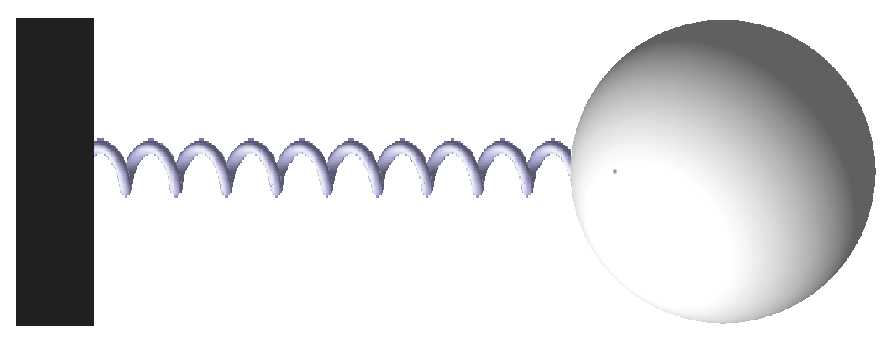
\includegraphics[width=2.5in]{FOM-springmass/springmass2smallest.eps}
\end{center}

The free end of the spring is allowed to move, and we need to impose coordinates on the figure to measure this motion.  There are many ways we could choose to do this.  The natural point to choose as an origin is the 
	\index{rest position}%
	{\bf rest position} of the free end of the spring -- that is to say, the point where the free end sits when the spring is not in a state of internal tension.  From this point, we can measure the displacement of the free end of the spring, and we shall adopt the convention that a stretched spring corresponds to a positive displacement, while a compressed spring corresponds to a negative displacement.

\begin{center}
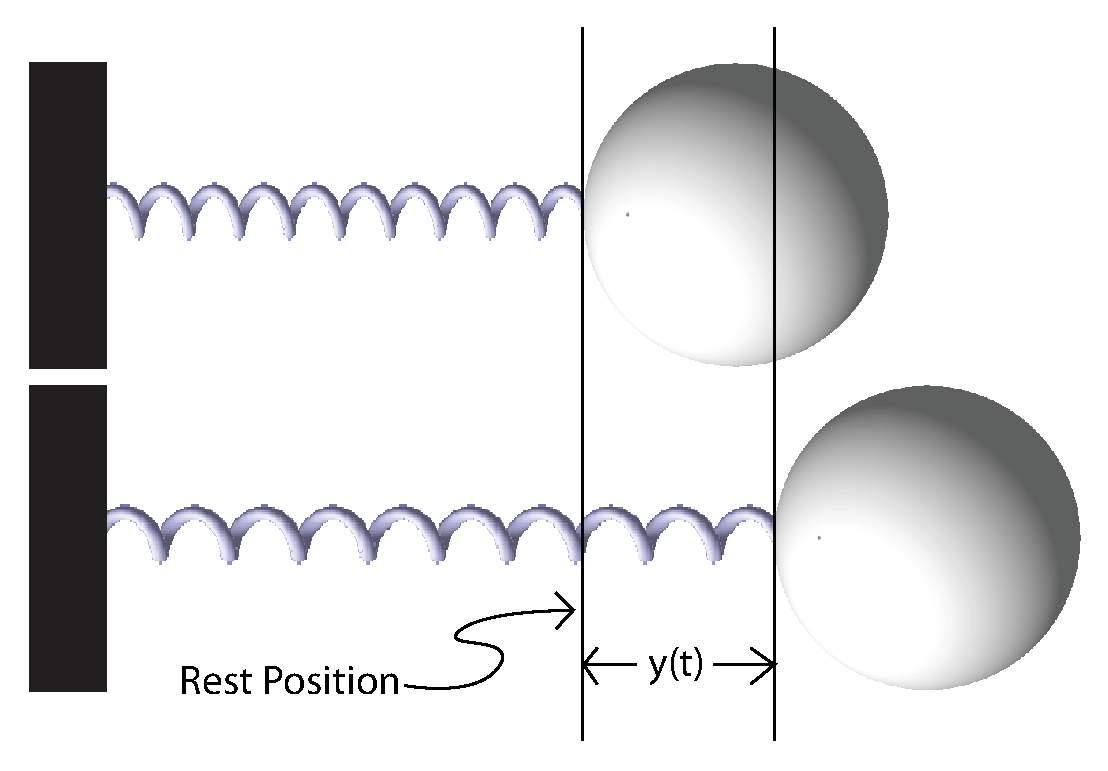
\includegraphics[width=3in]{FOM-springmass/springmassdisplacement.eps}
\end{center}

\hspace{0.125in}
To model the physical behavior of this system, our starting point is Newton's second law, $F=ma$ (force equals mass times acceleration).  If we let $y(t)$ denote the displacement of the free end of the spring from it's rest position as a function of time, then the acceleration is given by $\ddot{y}$.  There will also be at least two forces acting on the mass.  One is the spring's restoring force, which Hooke's Law tells us we can model by assuming it is proportional to the displacement from rest position: $F_s = -ky$.  (Here, the spring constant $k$ is positive, and the direction of the spring's restoring force is in the direction opposite the displacement.  Also, we will model the damping force by assuming it is proportional to the velocity of the mass (like viscous drag) and in the opposite direction: $F_d = -C\dot{y}$.  Let us denote any other external driving force by $F_e$, and suppose this driving force is described by a function of time, $F_e=f(t)$.  

\end{minipage}
}
\end{center}




\newpage
\thispagestyle{empty}

{\begin{center}
\psframebox[style=fombox]{\begin{minipage}{6in}



\hspace{0.125in}
With these conventions we have:
\[ ma=F_s+F_d+F_e\]
or
\[ m \ddot{y} = -ky - C \dot{y}+f(t),\]
which we rearrange as
\[ m \ddot{y} + C \dot{y} + k y = f(t).\]
We now see that this is a second order constant coefficient linear ODE, so we can study the behavior of this system using the mathematical techniques now available to us.  

\hspace{0.125in}
A standard choice of units for force would be Newtons, and a standard choice for measuring displacement $y$ would be meters.  Thus the spring constant could have units of $\frac{N}{m}$, indicating that the magnitude of the spring's restoring force is $k$ Newtons for each meter the spring is displaced from rest position.  If these units are used, then the last term on the left side of our ODE will have units of Newtons, which is consistent with the kind of units we would see on the right side of the equation for an external driving force $F_e$.  To maintain consistency with the other terms on the left side of the equation, we should select mass $m$ to be measured in kilograms, and time should be measured in seconds; that way the units of $m\ddot{y}$ will be $\frac{kg \cdot m}{s^2}$, which are the same as Newtons.  Similarly, the units of the damping coefficient will have to be $\frac{N \cdot s}{m}$.

\hspace{0.125in}
{\bf EXAMPLE:} Consider a mass of $3 \ kg$ attached to the end of a spring with spring constant $9 \frac{N}{m}$.  If there is no damping or outside driving force, and the mass is initially stretched $0.05 \ m$ from its rest position then released, determine how long it will take before the spring first returns to its rest position.  What will the velocity be at that instant?

\hspace{0.125in}
With the parameters $m=3$, $C=0$ and $k=9$, and the driving force $f(t)=0$, we are faced with the differential equation
\[ 3 \ddot{y} + 9 y = 0\]
and the initial conditions $y(0)=0.05$ and $\dot{y}(0)=0$.  The solution of this IVP is
\[ y(t) = 0.05 \cos (3t).\]
The free end of the spring will be at the rest position when $y(t)=0$, which will occurs when $3t = \frac{\pi}{2}+n\pi$, or $t=\frac{(2n+1)\pi}{6}$.  The smallest positive solution will be $t=\frac{\pi}{6}\approx 0.524 \ s$.  At that instant, the velocity will be $\dot{y} \left( \frac{\pi}{6} \right) = -0.15 \sin \left(\frac{\pi}{2} \right) = -0.15 \frac{m}{s}$.
\qed

\end{minipage}
}
\end{center}

 % FOCUS ON MODELING: SPRING-MASS SYSTEMS

\documentclass[12pt,letterpaper,twoside]{amsart}
\usepackage[latin1]{inputenc}
\usepackage{amsmath}
\usepackage{amsfonts}
\usepackage{graphicx}
\usepackage{amssymb}
\usepackage{multicol}
\usepackage{ulem}
\newcounter{example}
\newcounter{exercise}
\newcounter{problem}
\newcommand{\example}{\bigskip \noindent {\large {\sc Example \arabic{example}:}} \addtocounter{example}{1}}
\newcommand{\exercise}{\bigskip \noindent {\large {\sc Exercise \arabic{exercise}:}} \addtocounter{exercise}{1}}
\newcommand{\problem}{\bigskip \noindent {\large {\sc Problem \arabic{problem}:}} \addtocounter{problem}{1}}
\newcommand{\tech}{\marginpar{\vskip 10mm \begin{center}\includegraphics[width=0.25in]{calculatorimagesmall.eps} \end{center}}}
\newcommand{\solution}{\medskip \noindent {\bf Solution: }}
\newcommand{\R}{\mathbb{R}}





\begin{document}

\sffamily

%%%%  switch the commenting on this line and the next \chapter{Introduction}
\begin{center} {\LARGE The Method of Undetermined Coefficients} \end{center}

\setcounter{example}{1}
\setcounter{exercise}{1}


Now that we can solve second-order constant-coefficient linear homogeneous ODE of the form 
\[ a\ddot{y}+b\dot{y}+cy=0,\]
we would like to be able to solve the {\bf non-homogeneous} equations:
\[ a\ddot{y}+b\dot{y}+cy=f(t).\]
It is possible to write down general representation formulas for any continuous {\bf driving function} $f(t)$, but we will mostly be interested in the special cases when $f(t)$ is a polynomial, exponential or trigonometric function.

We will develop the idea of our technique in the following example.  Later examples will illustrate the streamlined version of this process.

\example Consider the differential equation 
\[y''+2y'+y=x^2.\]
We would like to find a general solution of this differential equation.  We will start by trying to find {\it one} solution.

What kinds of functions might satisfy the equation?  The driving function is a power function, and in order that a function, its derivative and second derivative might simplify on the left side of the ODE to just $x^2$, it would be a reasonable guess that some polynomial function might work.  We will therefore try to find a function of the form $y_p=Ax^2+Bx+C$ that satisfies the ODE.  (Notice that we don't want to try a polynomial of degree 3 or higher because there would be no way for the higher degree terms to cancel out and leave just $x^2$.)  Substitute this into the ODE to obtain
\begin{align*}
x^2 & = y_p''+2y_p'+y_p \\
& = (2A)+2(2Ax+B)+(Ax^2+Bx+C) \\
& = Ax^2 + (4A+B)x+(2A+2B+C)
\end{align*}
Equating the polynomial coefficients on both sides of the equation gives
\[ A=1, \ \ \ 4A+B=0, \ \ \ 2A+2B+C=0.\]
Consequently $A=1$, $B=-4$ and $C=6$.  Thus
\[ y_p (x) = x^2-4x+6\]
is one solution of the ODE.  Now let $y(x)$ be any solution of the equation, and define $y_h=y-y_p$.  Inserting this into the differential equation, we see that
\begin{align*}
x^2 & = y''+2y'+y \\
& = (y_h+y_p)''+2(y_h+y_p)'+(y_h+y_p) \\
& = y_h''+2y_h'+y_h + y_p''+2y_p'+y_p \\
& = y_h''+2y_h'+y_h + x^2
\end{align*}
Subtracting $x^2$ from both sides, we see that
\[ 0 = y_h''+2y_h'+y_h,\]
and we know how to solve this equation:
\[ y_h(x)=Ae^{-x}+Bxe^{-x}.\]
Consequently,
\[ y(x)=y_p(x)+y_h(x) =x^2-4x+6+Ae^{-x}+Bxe^{-x}.\]
All solutions of the ODE can be written in this form, so this is the general solution of the differential equation.
\qed

In the previous example, we too advantage of the following fact: if $y_p$ satisfies the non-homogeneous differential equation
\[ ay''+by'+cy=f(x)\]
and if $y_h$ is the general solution of the homogeneous equation
\[ ay''+by'+cy=0,\]
then $y=y_p+y_h$ is the general solution of the non-homogeneous ODE.  Based on this fact, we can try to find general solutions of non-homogeneous equations by finding just one solution (which we call a {\bf particular solution)} and then adding to it the general solution of the related homogeneous equation.

Our method for finding a particular solution was to guess a form of a particular solution (such as the polynomial $Ax^2+Bx+C$ we tried in the first example), and then by substituting it into the ODE we find the appropriate values for the unknown coefficients.  This approach is called the {\bf method of undetermined coefficients}.

\example {\bf Solve the IVP: $y''+y'-6y=3x+4$, $y(0)=1$, $y'(0)=0$.}

The homogeneous equation $y''+y'-6y=0$ has characteristic equation $r^2+r-6=0$, and the roots of this are $r=-3,2$.  Thus the homogeneous equation has the general solution $y_h=Ae^{-3x}+Be^{2x}$.  We guess that there might be a particular solution of the non-homogeneous equation of the form $y_p=Cx+D$.  Inserting this into the non-homogeneous equation yields
\[ 3x+4 = (0)+(C)-6(Cx+D) = -6Cx+(C-6D).\]
Equating coefficients gives us $C=-\frac{1}{2}$ and then $D=-\frac{7}{12}$.  This gives us $y_p=-\frac{1}{2}x-\frac{7}{12}$, and adding this to the general solution of the homogeneous equation yields the general solution of the non-homogeneous equation:
\[ y=-\frac{1}{2}x-\frac{7}{12}+Ae^{-3x}+Be^{2x}.\]
The initial conditions allow us to solve for $A$ and $B$:
\[ y(0)=1 \implies -\frac{7}{2} +A+B=1 \]
\[ y'(0)=0 \implies -\frac{1}{2}-3A+2B=0 \]
The solution of this system of algebraic equations is $A=\frac{17}{10}$ and $B=\frac{14}{5}$.  This gives us the solution of the IVP:
\[ y=-\frac{1}{2}x -\frac{7}{2}+\frac{17}{10}e^{-3x}+\frac{14}{5}e^{2x}.\]
\qed

\exercise Solve the initial value problem $y''-5y'+6y=x$, $y(0)=0$, $y'(0)=0$.

\exercise Try to find a particular solution to $y''+6y'=x$ of the form $y_p=Cx+D$.  End up proving that no such solution exists.

The last exercise shows us how we might need to be more clever when guessing the form of our particular solution.  If Any term in the driving function is a solution of the related homogeneous equation, we will need to modifythe form of our guess.  For the differential equation in the last exercise, the correct form of the guess is actually a degree-two polynomial.

\example Consider the ODE $y''+6y'=x$.  Let us seek a solution of the form $y_p=Cx^2+Dx$.  Insertin g this into the differential equation produces
\[ x=(2C)+6(2Cx+D)=12Cx+(2C+D).\]
Equating coefficients gives us $C=\frac{1}{12}$ and then $D=-\frac{1}{6}$.  Now we see that the function $y_p=\frac{1}{12}x^2-\frac{1}{6}x$ is a solution.
\qed

The general principle we follow here is this: if the driving term of the non-homogeneous equation is a polynomial (or a monomial) of degree $N$, then our guess for the form of a particular solution is 
\[ y_p=x^S q(x),\]
where $q(x)$ is a polynomial of degree $N$, and where $S \geq 0$ is the smallest non-negative integer such that no term in the polynomial $x^S q(x)$ is a solution of the related homogeneous equation.

Because we need to compare our guess with solutions of the related homogeneous equation, it is a good practice to find the general solution of the homogeneous equation first.

\exercise Find the general solution of $y''+2y'=x^2$.

We can employ the same techniques when the driving term is an exponential function.

\example {\bf Find the general solution of $y''+2y'+y=e^{2x}$.}

The characteristic equation is $r^2+2r+1=0$, which has a repeated root $r=-1$.  Thus the general solution of the related homogeneous equation is $y_h=Ae^{-x}+Bxe^{-x}$.  Next we guess that a particular solution of the non-homogeneous equation will have the form $y_p=Ce^{2x}$:
\[ e^{2x}=(4e^{2x})+2(2e^{2x})+(e^{2x}) = 9e^{2x},\]
so that $C=\frac{1}{9}$.  Therefore the general solution of the non-homogeneous equation is
\[ y=\frac{1}{9}e^{2x}+Ae^{-x}+Bxe^{-x}.\]
\qed

\example {\bf Find the general solution of $y''+2y'+y=e^{-x}$.}

The general solution of the related homogeneous equation is $y_h=Ae^{-x}+Bxe^{-x}$.  Therefore no multiple of $e^{-x}$ can be a solution of the non-homogeneous equations.  Also, nether can any multiple of $xe^{-x}$.  However, we can find a solution by looking for a multiple of $x^2e^{-x}$.  Let $y_p=Cx^2e^{-x}$.  Then $y_p'=C(2x-x^2)e^{-x}$ and $y_p''=C(2-4x+x^2)e^{-x}$.  Insert these into the ODE:
\begin{align*} e^{-x}& =\left(C(2-4x+x^2)e^{-x}\right)+2\left(C(2x-x^2)e^{-x}\right) +\left(Cx^2e^{-x}\right) \\
& = 2Ce^{-x}
\end{align*}
Thus $C=\frac{1}{2}$.  So $y_p=\frac{1}{2}x^2e^{-x}$ is a particular solution, and therefore the general solution is
\[ y=\frac{1}{2}x^2 e^{-x} +Ae^{-x}+Bxe^{-x}.\]
\qed

As in Example 3, when we recognized that the natural guess would be a solution of the homogeneous equation, we modified it by multiplying by the smallest power of $x$ such that the product would not be a homogeneous solution.  This same approach can applied when the driving terms is a sine or cosine function.  In general, if the driving term is $\sin(mx)$ or $\cos(mx)$, our guess will be a function of the form $y_p=Asin(mx)+B\cos(mx)$, unless we need to multiply by a power of $x$ to ensure that no term in our guess is a homogeneous solution.

\example {\bf Find a general solution of $y''-y=\sin(2x)$.}

The characteristic equation is $r^2-1=0$, which has solutions $r=\pm 1$; thus the solution of the homogeneous equation is $y_h=Ae^x+Be^{-x}$.  Now we guess that a solution of the non-homogeneous equation might have the form $y_p=C\sin(2x)+D\cos(2x)$.  Inserting this into the ODE yields
\begin{align*}
\sin(2x) & = \left(-4C\sin(2x)-4D\cos(2x)\right)-\left(C\sin(2x)+D\cos(2x) \right) \\
& = -5C\sin(2x)-5D\cos(2x).
\end{align*}
Equating coefficients gives us $C=-\frac{1}{5}$ and  $D=0$, so $y_p=-\frac{1}{5}\sin(2x)$.  The general solution is thus
\[ y=-\frac{1}{5}\sin(2x)+Ae^x+Be^{-x}.\]
\qed

\example {\bf Find a general solution of $y''+y=\sin(2x)$.}

The characteristic equation is $r^2+1=0$, which has solutions $r=\pm i$.  We thus write the general solution of the homogeneous equation as $y_h=A\sin(x)+B\cos(x)$.  Suppose a particular solution is $y_p=C\sin(2x)+D\cos(2x)$.  Then
\begin{align*}
\sin(2x)&=\left(-4A\sin(2x)-4B\cos(2x) \right) + \left(A\sin(2x)+\cos(2x) \right) \\
& = -3C\sin(2x)-3D\cos(2x).
\end{align*}
So $C=-\frac{1}{3}$ and $D=0$.  Thus $y_p=-\frac{1}{3}\sin(2x)$ and
\[ y = -\frac{1}{3}\sin(2x)+A\sin(x)+B\cos(x).\]
\qed

\example {\bf Find a general solution of $y''+y=\sin(x)$.}

As in the previous example, $y_h=A\sin(x)+B\cos(x)$.  Now, because the driving function $\sin(x)$ is a solution of the homogeneous equation, we use the guess $y_p=Cx\sin(x)+Dx\cos(x)$:
\begin{align*}
\sin(x) & = \left(2C \cos(x)-Cx\sin(x)-2D\sin(x)-D\sin(x)\right) \\
& \ \ \ \ \ \ \ \ \ \ +\left(Cx\sin(x)+Dx\cos(x) \right) \\
& = 2C\cos(x)-2D\sin(x).
\end{align*}
Therefore $C=0$ and $D=-\frac{1}{2}$, $y_p=-\frac{1}{2}x\cos(x)$ and 
\[ y = -\frac{1}{2}x\cos(x)+A\sin(x)+B\cos(x).\]
\qed

\exercise Find one solution for each of the following differential equations.
\begin{itemize}
\item $y''-y'+4y=x^2+1$
\item $y''+2y'+3y=\sin(3t)$
\item $y''+6y'=\cos(t)$
\item $\ddot{w}-\dot{w}-3w=e^{t}$
\item $v''+v=\sin(t)$
\item $y''-5y'+6y=e^{2x}$
\end{itemize}

\exercise Solve the following initial value problems.
\begin{itemize}
\item $y''+y=e^{3t}, \ y(0)=0, \ y'(0)=0$
\item $y''+6y'+9y=\sin(2t), \ y(0)=1, \ y'(0)=0$
\item $y''-4y=e^{-2t}, \ y(0)=0, y'(0)=0$
\end{itemize}

%% Cut below here for the book form.

\begin{center} {\LARGE Problems} \end{center}

\setcounter{problem}{1}

\problem Solve the IVP $y''+y=f(t), \ y(0)=0, y'(0)=2$, where $f$ is the function

\[ f(t) = \left\{ \begin{matrix} 0 & \mbox{for} \ t \leq \pi \\ t-\pi & \mbox{for} \ t > \pi \end{matrix} \right. .\]

{\it (Hint: Split this into two separate initial value problems -- one for $t \leq \pi$ and one for $t \geq \pi$.  You'll need to solve the first problme in order to know what initial conditions to use for the second problem.)}






\end{document} % SECOND ORDER NONHOMOGENEOUS


\input{9-oscillators/oscillators.chapter} % HARMONIC OSCILLATORS

\part{Laplace Transforms}

\documentclass[12pt,letterpaper,twoside]{amsart}
\usepackage[latin1]{inputenc}
\usepackage{amsmath}
\usepackage{amsfonts}
\usepackage{graphicx}
\usepackage{amssymb}
\usepackage{multicol}
\usepackage{ulem}
\newcounter{example}
\newcounter{exercise}
\newcounter{problem}
\newcommand{\example}{\bigskip \noindent {\large {\sc Example \arabic{example}:}} \addtocounter{example}{1}}
\newcommand{\exercise}{\bigskip \noindent {\large {\sc Exercise \arabic{exercise}:}} \addtocounter{exercise}{1}}
\newcommand{\problem}{\bigskip \noindent {\large {\sc Problem \arabic{problem}:}} \addtocounter{problem}{1}}
\newcommand{\tech}{\marginpar{\vskip 10mm \begin{center}\includegraphics[width=0.25in]{calculatorimagesmall.eps} \end{center}}}
\newcommand{\solution}{\medskip \noindent {\bf Solution: }}
\newcommand{\R}{\mathbb{R}}





\begin{document}

\sffamily

%%%%  switch the commenting on this line and the next \chapter{Introduction}
\begin{center} {\LARGE Laplace Transforms} \end{center}

\setcounter{example}{1}
\setcounter{exercise}{1}

In this chapter we will introduce the idea of a transform method.  The basic idea is this: we begin with an inial value problem for a differential equation, and we transform this equation into an algebraic equation; once we solve for the unknown in the algebraic equation, we then transform back to find a corresponding solution of the IVP.

The tool we will use for this is the {\bf Laplace Transform} of a function, defined by
\[ L[f]=\int_0^\infty f(t)e^{-st} \ dt.\]
Here, $f$ is a function defined on $[0,\infty)$ and $L[f]$ is a function of $s$ defined for whatever values of $s$ lead to a convergent integral.

\example The Laplace Transform of $e^{t}$ is
\begin{align*}
L[e^t]& =\int_0^\infty e^t e^{-st} \ dt \\
& = \lim_{T \rightarrow \infty} \int_0^T e^{(1-s)t} \ dt \\
& = \lim_{T \rightarrow \infty} \left. \frac{e^{(1-s)t}}{1-s} \right|_0^T \\
& = \lim_{T \rightarrow \infty} \frac{1}{1-s} - \frac{e^{(1-s)T}}{1-s} \\
& = \frac{1}{1-s} \ \ \ \mbox{for} \ s >1.
\end{align*}
\qed

\exercise Calculate the Laplace Transform of the functions $t^2$, $\sin(t)$ and $e^{at}$ (where $a$ is a constant).

\exercise Prove that the Laplace Transform is linear: for any functions $f$ and $g$ and for any constant coefficients $a$ and $b$, $L[af+bg]=aL[f]+bL[g]$.  {\it (This only needs to hold on the set of $s$-values for which $L[f]$ and $L[g]$ are both defined.)}

\bigskip
It is typical to denote a transform of a function with a capital letter.  For example, when it is useful to display the variable, we will often denote the Laplace Transform of a function $f(t)$ by $F(s)$; otherwise we will write it as $L[f]$.  We usually do not care what the exact domain is for $F(s)$ -- it will be enough to know that there is some interval for $s$ on which the integral defining the transform converges.  The next theorem provides such a guarantee.

{\bf Theorem: }
Suppose there exists $M\geq 0$ and $a>0$ such that $f(t) \leq Me^{at}$ for all $t \geq 0$.  Then the integral defining the Laplace Transform converges for all $s >a$.

A function that satisfies the hypothesis of this theorem is said to be of {\bf exponential order}, because it does not grow any faster than exponential functions can grow.

\bigskip
\proof

Observe that for $s>a$ we have
\begin{align*}
\int_0^\infty | f(t) e^{-st} | \ dt & = \int_0^\infty | f(t)| e^{-st} \ dt \\
& \leq \int_0^\infty Me^{at} e^{-st} \ dt \\
& =  \int_0^\infty M e^{(a-s)t} \ dt \\
& = \frac{M}{s-a} \\
& < \infty.
\end{align*}
This proves that the integral defining $L[f]$ converges absolutely for all $s > a$.
\qed



\bigskip
Next, we introduce the key fact which allows us to use Laplace Transforms for solving initial value problems.  There is a close relationship between the Laplace transform of a function and that of its derivative:

\begin{center}
\fbox{
\begin{minipage}{1.5in}
\[ L[ f' ] = s L [f] - f(0) \]
\end{minipage}
}
\end{center}

We call this a reduction formula for the Laplace Transform because it allows us to ``reduce''  $L[y']$ to an expression involving $L[y]$.

\bigskip
\noindent
{\bf Theorem:} If $L[f]$ exists for $s>a$, and if $\lim_{t \rightarrow \infty} f(t)e^{-st}=0$ for $s > a$, then $L[f']$ also exists for $s>a$ and $L[f']=sL[f]-f(0)$.

\bigskip
Notice that any function of exponential order satisfies both hypotheses of this theorem.

\bigskip
\proof We use integration by parts, integrating $f'(t)$ and differentiating $e^{-st}$:
\begin{align*}
L[f'] & = \int_0^\infty f'(t) e^{-st} \ dt \\
& = \lim_{T \rightarrow \infty} \int_0^T f'(t) e^{-st} \ dt \\
& = \lim_{T \rightarrow \infty} \left[ e^{-st} f(t) - \int -se^{-st} f(t) \ dt \right]_0^T \\
& = \lim_{T \rightarrow \infty} e^{-sT}f(T) - e^{0t} f(0) + s \int_0^T f(t) e^{-st} \ dt \\
& = -f(0) + s \int_0^\infty f(t) e^{-st} \ dt \\
& = -f(0)+sL[f].
\end{align*} 
\qed 

In practice, when faced with an unknown function we will always assume that it is of exponential order and therefore satisfies hypotheses of these two theorems.  Of course, in theory such an assumption could lead to erroneous results, but in practical applications this rarely happens.  And because the process we illustrate in the next few examples furnishes us with a concrete function, we can always check it to make sure it satisfies the differential equation at hand.

To make use of the Laplace Transform to solve an initial value problem, we need to make use of one more fact which we will not prove:

\bigskip
\noindent
{\bf Theorem:} If $f$ and $g$ are continuous functions on $[0,\infty)$ and $L[f]=L[g]$, then $f=g$.

\bigskip
The point of this theorem is that the Laplace Transform is invertible.  We denote the inverse by $L^{-1}$.  Because $L$ is linear, so is $L^{-1}$: 
\[ L^{-1}[aF(s)+bG(s)] = aL^{-1} [F(s)] + b L^{-1}[G(s)]\]

\example Since $L[e^{2t}]=\frac{1}{s-2}$, it follows that $L^{-1} \left[ \frac{1}{s-2} \right] = e^{2t}.$
\qed

\exercise Find $L^{-1} \left[ \frac{1}{s^3} \right]$.  {\it (Hint: Refer to Exercise 1.)}

We now have enough machinery to use the Laplace Transform for solving an IVP.

\example Suppose $y$ is a solution of $y'+2y=0, \ y(0)=3$ on the domain $[0,\infty)$.  We take the Laplace Transform of both sides of the ODE:
\[ L[y'+2y] = L[0].\]
Then we use the facts that $L$ is linear and $L[0]=0$:
\[ L[y']+2L[y]=0.\]
Next we apply the formula for the Laplace Transform of a derivative:
\[ sL[y]-y(0)+2L[y]=0.\]
Insert the initial condition $y(0)=3$ and collect like terms:
\[ (s+2)L[y]-3=0.\]
Isolate $L[y]$:
\[ L[y] = \frac{3}{s+2}.\]
Finally, isolate $y$ by taking the inverse Laplace Transform of both sides:
\begin{align*}
y & = L^{-1} \left[ \frac{3}{s+2} \right] \\
& = 3 L^{-1} \left[ \frac{1}{s-(-2)} \right] \\
& = 3 e^{-2t}.
\end{align*}
This is the solution of the IVP above.
\qed

Clearly it will be useful to have a list of functions and their corresponding Laplace Transforms.  Here is a short list of such correspondences.

\begin{center}
\begin{tabular}{c|c}
$f(t)$ & $F(s)$ \\ \hline
$t^n$ & $\frac{n!}{s^{n+1}}$ \\
$e^{at}$ & $\frac{1}{s-a}$ \\
$\sin(kt)$ & $\frac{k}{s^2+k^2}$ \\
$\cos(kt)$ & $\frac{s}{s^2+k^2}$ \\
$\sinh(kt)$ & $\frac{a}{s^2-k^2}$ \\
$\cosh(kt)$ & $\frac{s}{s^2-k^2}$ \\
$e^{at}\sin(bt)$ & $\frac{b}{(s-a)^2+b^2}$ \\
$e^{at}\cos(bt)$ & $\frac{s-a}{(s-a)^2+b^2}$\\
$ t^n e^{at}$ & $\frac{n!}{(s-a)^{n+1}}$
\end{tabular}
\end{center}

\exercise Use Laplace Transforms to solve the IVP $y'+4y=6, \ y(0)=2$.    
 


Higher-order ODE can be solved in the same way.  When we transform $y''$, we just use the reduction formula twice:
\[ L[y'']=sL[y']-y'(0)=s(sL[y]-y(0))-y'(0)=s^2L[y]-sy(0)-y'(0).\]
The reader may choose to memorize this formula as well, or just to use the first-order formula repeatedly when required.

\example {\bf Solve the IVP $y''+9y=2, \ y(0)=1, \ y'(0)=0$.}

Transform both sides of the equation, rewrite all the Laplace Transforms in terms of $L[y]$, and then isolate $L[y]$:

\begin{align*}
L[y''+9y]=L[2] \\
L[y'']+9L[y]=\frac{2}{s} \\
sL[y']-y'(0)+9L[y]=\frac{2}{s} \\
s(sL[y]-y(0))-y'(0)+9L[y]=\frac{2}{s} \\
(s^2+9)L[y]-s-0=\frac{2}{s}\\
(s^2+9)L[y]=s+\frac{2}{s} \\
L[y]=\frac{s}{s^2+9}+\frac{2}{s(s^2+9)}
\end{align*}

Use a partial fractions decomposition to rewrite the right side of the equation:
\begin{align*} 
L[y]& =\frac{s}{s^2+9}+\frac{(2/9)}{s}+\frac{(-2/9)s}{s^2+9} \\
& = \frac{(7/9)s}{s^2+9}+\frac{(2/9)}{s}
\end{align*}
Then isolate $y$ using the inverse transform:
\begin{align*}
y & = L^{-1} \left[ \frac{(7/9)s}{s^2+9}+\frac{(2/9)}{s} \right] \\
& = \frac{7}{9} L^{-1} \left[ \frac{s}{s^2+9} \right] + \frac{2}{9} L^{-1} \left[ \frac{1}{s} \right] \\
& = \frac{7}{9} \cos(3t) +\frac{2}{9}
\end{align*}
\qed


\exercise Use Laplace Transforms to solve the IVP $y''+25y=t$, $y(0)=0$, $y'(0)=3$.

\exercise Use Laplace Transforms to solve the IVP $y''+4y'=6, \ y(0)=0, \ y'(0)=1$.    

\exercise Use Laplace Transforms to solve the IVP $y''-6y'+8y=6, \ y(0)=2, y'(0)=0$.   

\exercise Use Laplace Transforms to solve the IVP $y''+4y'+4y=\sin(t), \ y(0)=0, y'(0)=0$.



%% Cut below here for the book form.

\begin{center} {\LARGE Problems} \end{center}

\setcounter{problem}{1}


\problem Prove that, if $L[f(t)]=F(s)$, then $L[t^nf(t)]=(-1)^n F^{(n)}(s)$.  {\it (Hint: Use integration by parts.)}


\problem Prove all the formulas for the Laplace Transform given in the table in this chapter.

\problem Another useful transform in the study of differential equations is the Fourier Transform which can be defined for a function $f(t)$ by the formula $F[f] = \int_{-\infty}^\infty f(t) e^{-2\pi i \xi t} \ dt$.  (Here, the transform is a function of $\xi$.)  Verify the following reduction formula for differentiable functions $f$ that satisfy $\lim_{t \rightarrow \pm \infty}f(t)=0$:
\[ F[f'] = \frac{1}{2 \pi i} F[f].\]

\problem Prove that $f(t)=e^{(t^2)}$ {\it is not} of exponential order.

 






\end{document} % LAPLACE TRANSFORMS

\chapter{Discontinuous Driving Functions}

\setcounter{example}{1}
\setcounter{exercise}{1}



{\begin{center}
\psframebox[style=profibox]{\begin{minipage}{4in}
{\bf Prototype Question:} 
	\index{spring-mass system}%
	Model the effect on a spring-mass system when the mass is hit with a hammer.
\end{minipage}
}
\end{center}



In this chapter we explore the type of initial value problems for which Laplace Transforms are our best-suited tool: non-homogeneous equations with discontinuous driving functions.

\bigskip
\noindent
{\large {\sc Unit Step Functions and Characteristic Functions}}

\bigskip
The 
	\index{unit step function}%
	{\bf unit step function} is defined by
\[ \mathcal{U}(t) = \left\{ \begin{matrix} 0 & \mbox{for} \ t < 0 \\ 1 & \mbox{for} \ t > 0 \end{matrix} \right. .\]
Notice that we do not bother defining $\mathcal{U}(0)$.  That is because there is no natural way to define it that will be of practical value.  Furthermore, we will mainly use these step functions inside integrands, and the value of a function at one point will not affect the definite integral.

We also define $\mathcal{U}_a$ as a translation of the unit step function $a$ units to the right (if $a<0$, the translation would actually be to the left):
\[ \mathcal{U}_a(t) = \left\{ \begin{matrix} 0 & \mbox{for} \ t < a \\ 1 & \mbox{for} \ t>a \end{matrix} \right. .\]

\begin{exe} Prove that $L[\mathcal{U}_a ] = \left\{ \begin{matrix} \frac{1}{s} & \mbox{for} \ a \leq 0 \\ \frac{e^{-as}}{s} & \mbox{for} \ a > 0 \end{matrix} \right. $.
\end{exe}

Unit step functions can be used to describe driving functions which are ``switched on'' at a certain moment in time.  For example, a differential equation of the form $a\ddot{y}+b\dot{y}+cy=E(t)$ can be used to model the current in a simple electrical circuit, where $E(t)$ is the driving term corresponding to an external voltage source.  If a 12-volt source is ``turned on'' at time $t=2$ seconds, then we could model this with a driving term $E(t)=12\mathcal{U}_2(t)$, which is illustrated in the following figure.
\begin{center}
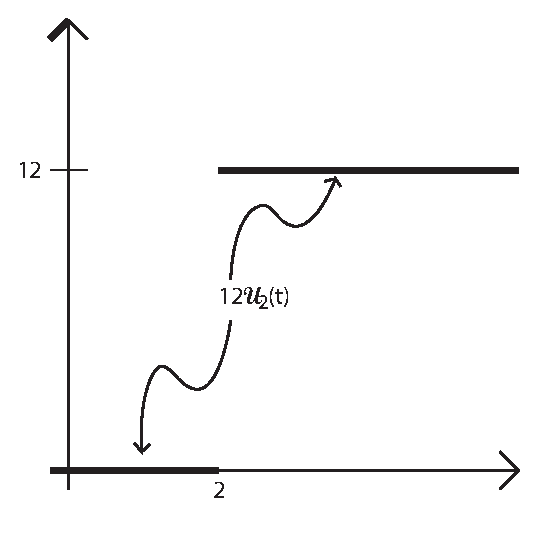
\includegraphics[width=2.25in]{11-laplaceII/stepfunction1.eps}
\end{center}

\begin{exe} Sketch the graphs of {\bf (a)} $f(t) = 2\mathcal{U}_1(t)$, {\bf (b)} $g(t)= 1+2\mathcal{U}_1(t)$ and {\bf (c)} $h(t) = 3-2\mathcal{U}_1(t)$.  
\end{exe}

Expanding on the example of a voltage source described above, we could also imagine that the voltage source is ``turned off' at, say, $t=8$ seconds, as shown here:
\begin{center}
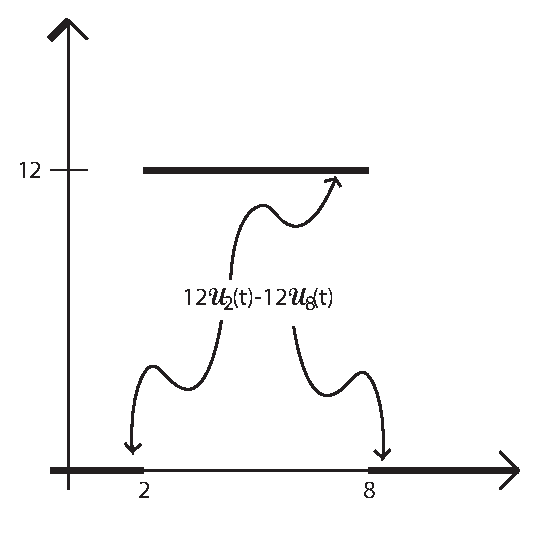
\includegraphics[width=2.25in]{11-laplaceII/stepfunction2.eps}
\end{center}
The function $E(t)$ shown in the last figure can be represented as a difference of step functions by writing $E(t) = 12 \mathcal{U}_2(t) - 12 \mathcal{U}_8(t)$.  We can think of the first term, $12 \mathcal{U}_2(t)$, as ``stepping up'' by 12 units at $t=2$, and the second term, $-12\mathcal{U}_8(t)$, as ``stepping back down'' at $t=8$.

More generally, we can represent any function of the form 
\[f(t) = \begin{cases} c & \mbox{if } a < t < b \\ 0 & \mbox{otherwise} \end{cases}\] 
as a difference of step functions: $f(t) = c\mathcal{U}_a - c \mathcal{U}_b$.  It is often useful to think of this as a basic building block for other functions, so we give it a name and its own notation: the function $\mathcal{U}_{a,b}(t)$ defined by 
\[ \mathcal{U}_{a,b}(t) = \mathcal{U}_a(t) - \mathcal{U}_b(t) = \begin{cases} 1 & \mbox{if } a < t < b \\ 0 & \mbox{otherwise} \end{cases}\]
is called the %
	\index{characteristic function}%
	{\bf characteristic function} (or the %
	\index{indicator function}%
	{\bf indicator function}) {\bf of the interval $(a,b)$}.
Although we will use this notation at times to help us come up with a formula for a function, we will always choose to write our final answers in terms of step functions instead of characteristic functions.

\begin{exe} Find a formula in terms of step functions for the function shown in the figure below.  {\it (Hint: Begin by thinking of this as a sum of two characteristic functions.  Then write the characteristic functions in terms of step functions and simplify.)}
\begin{center}
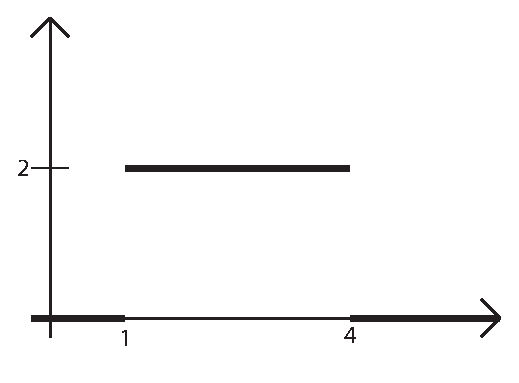
\includegraphics[width=2.25in]{11-laplaceII/stepfunction6.eps}
\end{center}
\end{exe}

\begin{exe} Find a formula in terms of step functions for the function shown in the figure below.
\begin{center}
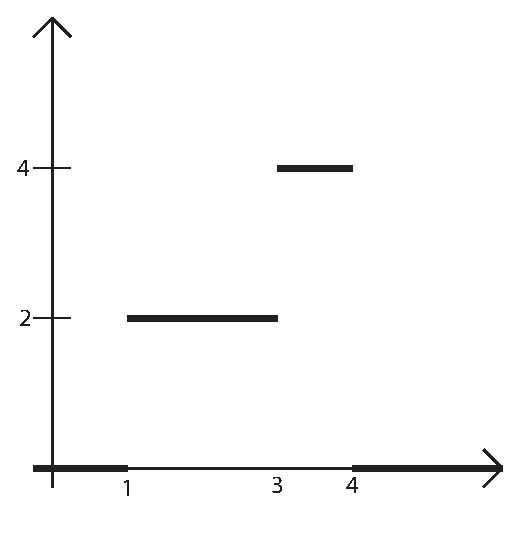
\includegraphics[width=2.25in]{11-laplaceII/stepfunction3.eps}
\end{center}
\end{exe}




When we multiply a function $f(t)$ by a unit step function $\mathcal{U}_a(t)$, the resulting product gives us the same output as $f$ when $t>a$, and the output is $0$ when $t<a$.  For example, here's a sketch of the graph of $g(t)=t^2 \mathcal{U}_0(t)$:

\begin{center}
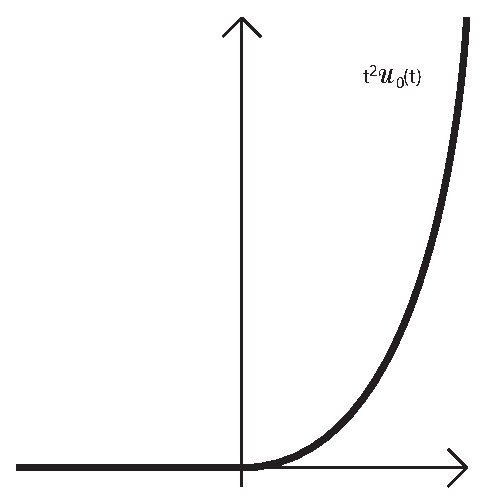
\includegraphics[width=2.25in]{11-laplaceII/stepfunction4.eps}
\end{center}

\begin{exe} Sketch the graphs of {\bf (a)} $f(t)=t \mathcal{U}_3(t)$ and {\bf (b)} $(t-3) \mathcal{U}_3(t)$.
\end{exe}

\example Sketch a graph of the function 
\[ f(t) = \begin{cases} 1-(t-2)^2 & \mbox{if } 1 < t < 3 \\ 0 & \mbox{otherwise} \end{cases},\] 
and write a formula for $f(t)$ in terms of step functions.

\medskip
\noindent
\begin{minipage}{4in}
\hspace{0.25in} The graph of $f$ is shown in the figure at right.  This function can be thought of as a product with the characteristic function of the interval $(1,3)$:
\begin{align*}
f(t) & = (1-(t-2)^2)\mathcal{U}_{1,3}(t) \\
& = (1-(t-2)^2)\left( \mathcal{U}_1(t) - \mathcal{U}_3(t) \right).
\end{align*}
\end{minipage}
\hspace{0.25in}
\begin{minipage}{2in}
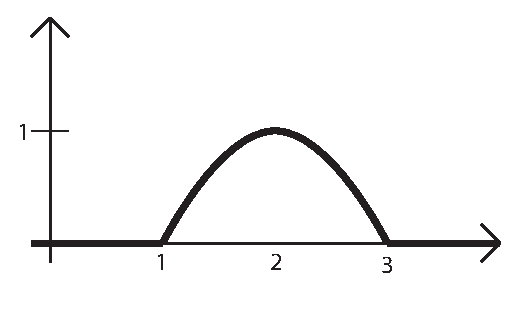
\includegraphics[width=2in]{11-laplaceII/stepfunction7.eps}
\end{minipage}

\qed

\begin{exe} Find formulas in terms of step functions for the functions whose graphs are shown in the following figures.  

\begin{center}
{\bf (a)} 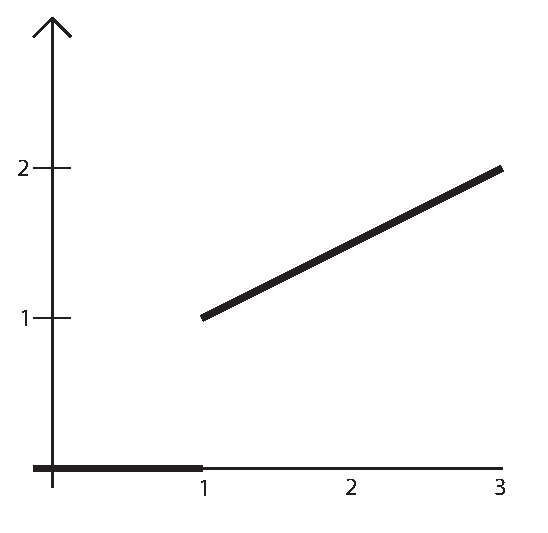
\includegraphics[width=2.25in]{11-laplaceII/stepfunction5.eps} \hspace{0.25in} {\bf (b)} 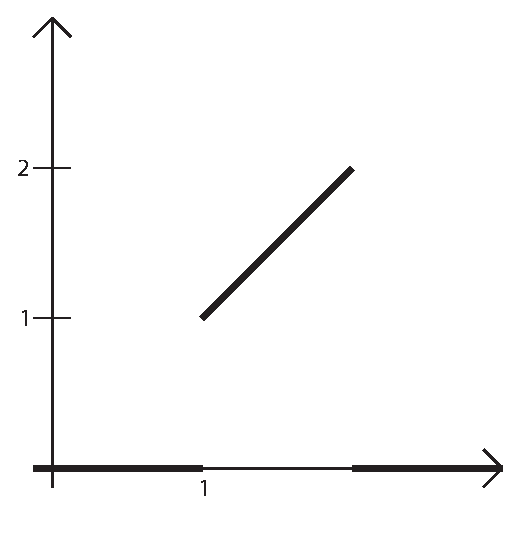
\includegraphics[width=2.25in]{11-laplaceII/stepfunction5b.eps}
\end{center}
\end{exe}

\bigskip
\noindent
{\large {\sc Step Functions and Translations of Functions}}

\bigskip
Unit step functions are particularly useful when we try to work with Laplace Transforms of functions which have been translated.  Observe that, for a function $f(t)$, the Laplace Transform of $f(t-a)$ is not necessarily very simple, as this calculation shows:
\begin{align*}
L[f(t-a)] & = \int_0^\infty f(t-a)e^{-st} \ dt \\
& = \int_{-a}^\infty f(u) e^{-s(u+a)} \ du \ \ \ \ \ (u=t-a, \ du=dt) \\
& = \int_{-a}^0 f(u) e^{-s(u+a)} \ du + \int_0^\infty f(u)e^{-su}e^{-as} \ du \\
& = \int_{-a}^0 f(u) e^{-s(u+a)} \ du + e^{-as} L[f(t)].
\end{align*}

If the first integral in the last line is complicated, this may not be very useful.  On the other hand, if the first integral in the last line were just zero, it wouldn't be very complicated at all!  So to make sure that it is zero, when we translate a function $a$ units, as in $f(t-a)$, we will also multiply it by $\mathcal{U}_a$ (this is equivalent to imagining that $f(t)=0$ for $t<0$ before it is translated):


\begin{align*}
L[f(t-a)\mathcal{U}_a(t) ] & = \int_0^\infty f(t-a) \mathcal{U}_a(t) e^{-st} \ dt \\
& = \int_0^a f(t-a)\cdot 0 \cdot e^{-st} \ dt + \int_a^\infty f(t-a) \cdot 1 \cdot e^{-st} \ dt \\
& = \int_a^\infty f(t-a) e^{-st} \ dt \\
& = \int_0^\infty f(u) e^{-s(u+a)} \ dt \ \ \ \ \ (u=t-a, \ du=dt) \\
& = e^{-as} \int_0^\infty f(u) e^{-su} \ du \\
& = e^{-as} L[f(t)].
\end{align*}

The calculation above says that $L[\mathcal{U}_af(t-a)]=e^{-as}L[f(t)]$; however, this formula seems to be difficult for many students to remember and use correctly in this form.  To simplify it, let's introduce a 
	\index{shift-and-cutoff operator}
	{\bf shift-and-cutoff} operator, $S_a$, which acts on functions as follows: if $f$ is a function defined on $\mathbb{R}$, then $S_a(f)$ is another function defined on $\mathbb{R}$ according to the rule
\[ S_a(f)(t) = \begin{cases} f(t-a) & \mbox{if } t > a \\ 0 & \mbox{if } t < a \end{cases}.\]
The effect of the operator $S_a$ is to shift the graph $a$ units to the right and the ``cutoff'' the function by setting it equal to zero for all $t < a$.  

Thus, $S_a(f)(t)$ is also equal to $\mathcal{U}_a (t) f(t-a)$, which means that the rule we calculated above can be expressed as follows:

{\begin{center}
\psframebox[style=formulabox]{\begin{minipage}{4.5in}
{\bf {\color{OliveGreen} Laplace Transform of a Shifted-and-Cutoff Function \normalcolor}}
\index{Laplace Transform of a shifted-and-cutoff function}
\[ L[S_a(f)] = e^{-as}L[f].\]
\end{minipage}
}
\end{center}



\example The Laplace Transform of $f(t)=(t-3)^2\mathcal{U}_3 (t)$ is
\begin{align*}
L[(t-3)^2\mathcal{U}_3(t)] & = L[S_3 \left( t^2 \right)] \\
& = e^{-3s}L[t^2] \\
& = e^{-3s} \frac{2}{s^3}.
\end{align*}
\qed

\begin{exe}
Find the Laplace Transform of the function in the figure below by expressing it as $S_a(t)$ (a shift-and-cutoff of the linear function $t$) for some appropriate value of $a$.
\begin{center}
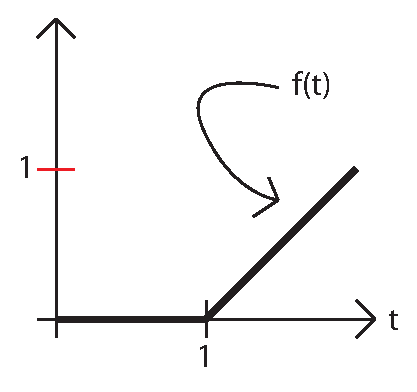
\includegraphics[width=2.5in]{11-laplaceII/figure1.eps}
\end{center}
\end{exe}


The corresponding rule for the Inverse Laplace Transform can be stated as follows: If $L^{-1}[F(s)]=f(t)$, then $L^{-1}[e^{-as}F(s)] = f(t-a)\mathcal{U}_a(t)$.  In terms of the shift-and-cutoff operator, we write the rule as follows:
{\begin{center}
\psframebox[style=formulabox]{\begin{minipage}{4.5in}
{\bf {\color{OliveGreen} Inverse Laplace Transform of $e^{-as}F(s)$ \normalcolor}}
\index{Inverse Laplace Transform with shifted-and-cutoff function}
\[ L^{-1} [ e^{-as}F(s)] = S_a \left( L^{-1}[F(s)] \right) = S_a (f), \mbox{where} f=L^{-1}[F]\]
\end{minipage}
}
\end{center}


\example The Inverse Laplace Transform of $F(s)=\frac{e^{-2s}}{s-4}$ is $e^{4(t-2)}\mathcal{U}_2(t)$.  We obtain this by recognizing that the Inverse Laplace Transform of $\frac{1}{s-4}$ is $e^{4t}$, which we then translate to the right by two units and multiply by the step function $\mathcal{U}_2$:
\begin{align*}
L^{-1} \left[e^{-2s}\frac{1}{s-4} \right] & = S_2 \left( L^{-1} \left[ \frac{1}{s-4} \right] \right) \\
& = S_2 \left( e^{4t} \right) \\
& = e^{4(t-2)}\mathcal{U}_2(t).
\end{align*}
\qed

\begin{exe}
Find the Inverse Laplace Transform of $F(s)=\frac{e^{-4s}}{s^3}$.
\end{exe}

We are now ready to use these step functions as driving functions in differential equations.

\example Solve the differential  equation $\dot{y}-y = \begin{cases} 0 & \mbox{if } t < 1 \\ 2 & \mbox{if } t > 1 \end{cases}$ subject to the initial condition $y(0)=0$.

{\bf Solution:} First, we rewrite the driving function as $2\mathcal{U}_1(t)$.  Then we transform the differential equation:
\begin{align*}
L [ \dot{y} - y ] & = L [ 2\mathcal{U}_1(t)] \\
L[\dot{y}] - L[y] & = 2 \frac{e^{-s}}{s} \\
s L[y]-y(0)-L[y] & = 2 \frac{e^{-s}}{s}
\end{align*}
where we used the reduction formula for $L[\dot{y}]$ in the last line.  Now plug in the initial condition $y(0)=0$, collect like terms and isolate $L[y]$:
\[ (s-1)L[y] = 2 \frac{e^{-s}}{s}\]
so
\[ L[y] = 2e^{-s} \left( \frac{1}{s(s-1)} \right).\]
We can use partial fractions to rewrite the expression in parentheses on the right:
\[ L[y] = 2e^{-s} \left( \frac{1}{s-1}-\frac{1}{s} \right).\]
Therefore
\begin{align*}
y & = 2S_1 \left( L^{-1} \left[ \frac{1}{s-1}-\frac{1}{s} \right] \right) \\
& = 2S_1 \left( e^t -1 \right) \\
& = 2 \left( e^{t-1}-1 \right) \mathcal{U}_1(t).
\end{align*}
It is often more useful (and more pleasant) to express the result in piecewise notation, without the step function:
\[ y = \begin{cases} 0 & \mbox{if } t < 1 \\ 2(e^{(t-1)}-1) & \mbox{if } t > 1 \end{cases}.\]
\qed

\example Solve the initial value problem $\dot{y}+y = \begin{cases} 0 & \mbox{if } t<5 \\ 2(t-5) & \mbox{if } t > 5 \end{cases}$, $y(0)=0$.

{\bf Solution:} The driving function can be written as $f(t)=2(t-5)\mathcal{U}_5(t)$, or $f(t)=S_5(2t)$, so we have
\[ \dot{y} + y = S_5(2t).\]
Taking Laplace Transforms of both sides gives us
\[ L [ \dot{y} ] + L[y] = L[S_5(2t)],\]
or
\[ sL[y]-y(0)+L[y] = e^{-5s} L[2t],\]
and thus
\[ (s+1)L[y] = e^{-5s}\frac{2}{s^2}.\]
Isolating $L[y]$ gives us
\[ L[y] = e^{-5s} \frac{2}{s^2(s+1)}.\]
A partial fraction decomposition for $\frac{2}{s^2(s+1)} = \frac{As+B}{s^2} + \frac{C}{s+1}$ gives us the coefficients $A=-2, \ B=2, \ C=2$, so we have
\[ L[y] = e^{-5s} \left( \frac{-2s+2}{s^2} + \frac{2}{s+1} \right).\]
Splitting up the first fraction inside parentheses on the right side and simplifying yields
\[ L[y] = e^{-5s} \left( \frac{-2}{s} + \frac{2}{s^2} + \frac{2}{s+1} \right).\]
Taking the Inverse Laplace Transform now gives us
\[ y = S_5 \left( -2 + 2t+2e^{-t} \right).\]
In piecewise notation, this is
\[ y = \begin{cases} 0 & \mbox{if } t<5 \\ -2 + 2(t-5) + 2e^{-(t-5)} & \mbox{if } t >5 \end{cases}.\]
\qed



\begin{exe} 
Solve the following initial value problems using Laplace Transforms:

{\bf (a)} $\dot{y}+2y = \begin{cases} 0 & \mbox{if } t < 1 \\ 9 & \mbox{if } t > 1 \end{cases}$, $y(0)=0$ 

{\bf (b)} $\dot{y}-y = \begin{cases} 0 & \mbox{if } t < 1 \\ (t-1)^2 & \mbox{if } t > 1 \end{cases}$, $y(0)=0$.
\end{exe}

In typical applications, Laplace Transforms are frequently used to solve second-order problems.  The process is generally the same.  

\example Solve the initial value problem $\ddot{y}-y=f(t), \ y(0)=0, \dot{y}(0)=1$, where the driving function is 
\[ f(t) = \left\{ \begin{matrix} 0 & \mbox{for} \ t<2 \\ 1 & \mbox{for} \ 2 <t<5 \\ 0 &\mbox{for} \ t>5 \end{matrix} \right. .\]

{\bf Solution:} We rewrite the driving function as $f(t)=\mathcal{U}_2 - \mathcal{U}_5$.  Then we transform the differential equation:
\begin{align*}
L[\ddot{y} -y] &= L[\mathcal{U}_2 - \mathcal{U}_5] \\
L[\ddot{y}] -L[y] &= L[\mathcal{U}_2] - L[\mathcal{U}_5] \\
sL[\dot{y}-\dot{y}(0)-L[y] &= \frac{e^{-2s}}{s}-\frac{e^{-5s}}{s} \\
s(sL[y]-y(0))-\dot{y}(0)-L[y] & = \frac{e^{-2s}}{s}-\frac{e^{-5s}}{s}.
\end{align*}
Then insert the initial conditions and solve for $L[y]$:
\begin{align*}
s(sL[y]-0)-1-L[y] & = \frac{e^{-2s}}{s}-\frac{e^{-5s}}{s} \\
(s^2-1)L[y] & = 1+ \frac{e^{-2s}}{s}-\frac{e^{-5s}}{s} \\
L[y] & = \frac{1}{s^2-1} + (e^{-2s}-e^{-5s}) \left( \frac{1}{s(s^2-1)}\right).
\end{align*}
We will need two partial-fractions decompositions:
\[ \frac{1}{s^2-1}= \frac{(1/2)}{s-1}-\frac{(1/2)}{(s+1)}\]
and
\[ \frac{1}{s(s^2-1)}= -\frac{1}{s} + \frac{(1/2)}{s-1} + \frac{(1/2)}{s+1} .\]
Insert these into the formula for $L[y]$ to obtain
\begin{align*}
L[y] & = \frac{(1/2)}{s-1}-\frac{(1/2)}{(s+1)} + (e^{-2s}-e^{-5s})\left( -\frac{1}{s} + \frac{(1/2)}{s-1} + \frac{(1/2)}{s+1} \right) \\
& = \frac{(1/2)}{s-1}-\frac{(1/2)}{(s+1)} 
+ e^{-2s} \left( -\frac{1}{s} + \frac{(1/2)}{s-1} + \frac{(1/2)}{s+1} \right) \\
& \ \ \ \ \ \ \ \ \ \ \ \ \ \ \ \ \ \ \ \ -e^{-5s} \left( -\frac{1}{s} + \frac{(1/2)}{s-1} + \frac{(1/2)}{s+1} \right). \\
\end{align*}
Consequently,
\begin{align*}
y(t) & = \frac{1}{2}e^{t} - \frac{1}{2}e^{-t} +S_2\left( -1 +\frac{1}{2}e^{t}+\frac{1}{2}e^{-t} \right) -S_5\left( -1 +\frac{1}{2}e^{t}+\frac{1}{2}e^{-t} \right) \\
& = \frac{1}{2}e^{t} - \frac{1}{2}e^{-t} +\left( -1 +\frac{1}{2}e^{(t-2)}+\frac{1}{2}e^{-(t-2)} \right) \mathcal{U}_2(t) -\left( -1 +\frac{1}{2}e^{(t-5)}+\frac{1}{2}e^{-(t-5)} \right) \mathcal{U}_5(t) \\
& = \left\{ \begin{matrix} \frac{1}{2}e^t -\frac{1}{2}e^{-t} & \mbox{for} \ t < 2 \\ \frac{1}{2}e^t -\frac{1}{2}e^{-t}-1 +\frac{1}{2}e^{(t-2)}+\frac{1}{2}e^{-(t-2)} & \mbox{for} \ 2<t < 5 \\ \frac{1}{2}e^t -\frac{1}{2}e^{-t} +\frac{1}{2}e^{(t-2)}+\frac{1}{2}e^{-(t-2)} -\frac{1}{2}e^{(t-5)}-\frac{1}{2}e^{-(t-5)} & \mbox{for} \ t >5 \end{matrix} \right. .
\end{align*}
\qed



\begin{exe}
Solve the following initial value problems using Laplace Transforms:

{\bf (a)} $\ddot{y}+4y = \begin{cases} 0 & \mbox{if } t < \pi \\ 1 & \mbox{if } t > \pi \end{cases}, \ y(0)=0, \ \dot{y}(0)=0$

{\bf (b)} $\ddot{y}+4y = \begin{cases} 1 & \mbox{if } t < \pi \\ 0 & \mbox{if } t > \pi \end{cases}, \ y(0)=0, \ \dot{y}(0)=0$

{\bf (c)} $\ddot{y}+y = \begin{cases} 0 & \mbox{if } t < 2 \\ 3(t-2) & \mbox{if } t > 2 \end{cases}, \ y(0)=0, \ \dot{y}(0)=0$.
\end{exe}






\bigskip
\noindent
{\large {\sc Delta (Impulse) Functions}}

\bigskip
Step functions can be used to describe driving functions that `start' or `stop' at definite instants in time, such as when a switch is closed for a certain time interval allowing an external voltage source to drive the circuit.  But we also sometimes want to model very short bursts of driving activity, such as a near-instantaneous jolt, and it turns out that the best means for this is with a so-called delta function.

The 
	\index{delta function}%
	{\bf delta function with pole at $a$} is denoted by $\delta_a(x)$ and is defined by the following property:
\[ \int_I f(x) \delta(x) \ dx = \begin{cases} f(a) & \mbox{if } a \in I \\ 0 & \mbox{if } a \notin I \end{cases}\]
for all continuous functions $f$ and for all intervals $I \subset \mathbb{R}$.  We will sometimes write $\delta$ in place of $\delta_0$.  Then we can also interpret $\delta_a(x)$ as $\delta(x-a)$.

An immediate consequence of this definition, if we use the constant function $f(x)=1$, is that
\[\int_{-\infty}^\infty \delta(x) \ dx = 1,\]
however, on any interval $I$ that does not contain $0$,
\[ \int_I \delta(x) \ dx = 0.\]

Thinking in terms of areas under the graph of $\delta$, it should not take the reader long to realize that this is impossible -- that there is no {\it function} which can have both of these properties.  Indeed, $\delta_a$ is actually a {\it distribution} (also called a {\it generalized function}).    In contrast to functions which have a defined value at each point of their domains, often distributions can only be thought of as having average values over intervals.

Distributions are often studied in detail in an advanced course on Functional Analysis.  Once defined, distributions can be multiplied by smooth functions, and the results can be integrated on intervals, but defining distributions carefully and illustrating just how all of this works in detail is well beyond the scope of this textbook.  At this level, all we will need are the two properties described above and their consequences.

To illustrate the utility of this object as a driving function, let's consider the differential equation $\ddot{y}=\delta_2(t)$, with the initial conditions $y(0)=0$ and $\dot{y}(0)=0$.  Because this is a fairly uncomplicated differential equation, we can solve it just by integrating.  Integrate both sides over the interval $(0,t)$ (let's use $s$ as the variable of integration) to get
\[ \int_0^t \ddot{y}(s) \ ds = \int_0^t \delta_2(s) \ ds.\]
The left side is just $\dot{y}(t) - \dot{y}(0)$, and the initial condition $\dot{y}(0)=0$ allows us to just write the left side as $\dot{y}(t)$, so we have $\dot{y}(t) = \int_0^t \delta_2(s) \ ds$.

The right side of the equation is now either equal to 1 (if the domain of integration includes 2) or 0 (if it does not).  The domain of integration includes 2 if $t>2$, so we can actually write the right side as $\mathcal{U}_2(t)$.  Therefore
\[ \dot{y}(t) = \mathcal{U}_2(t).\]
Let's integrate one more time to finish up:
\[ \int_0^t \dot{y}(s) \ dt = \int_0^t \mathcal{U}_2(s) \ ds,\]
and the left side will simplify to just $y(t)$ (since $y(0)=0$); the right side will simplify to 0 if $t<2$, and if $t>2$ then the right side will be 
\[ \int_0^t \mathcal{U}_2(s) \ ds = \int_0^2 \mathcal{U}_2(s) \ ds + \int_2^t \mathcal{U}_2(s) \ ds = 0 + \int_2^t 1 \ ds = (t-2).\]
Therefore we have
\[ y(t) = (t-2) \mathcal{U}_2(t) = \begin{cases} 0 & \mbox{if } t < 2 \\ (t-2) & \mbox{if } t > 2 \end{cases}.\]

This example illustrates how a delta function for a driving term provides an instantaneous change to the first derivative of the solution.  (Notice how $\dot{y}$ above changes from 0 to 1 exactly at $t=2$.)  One way to visualize this is with a spring-mass system, and to think of the driving function provided by $\delta_a$ as representing the hitting the mass with a hammer at time $t=a$, imparting a sudden change in the mass' momentum.  In the language of physics, we would say that, as a driving function, $\delta_a$ imparts one unit of impulse to the system (in physics, 
	\index{impulse}%
	{\bf impulse} is a constant force multiplied by time, or a non-constant force integrated over an interval of time).  Because of this physical interpretation, $\delta$ is also called an 
	\index{impulse function}%
	{\bf impulse function}.

A unit of impulse could be imparted by a constant force over a given time interval.  For example, the driving function $\mathcal{U}_1 - \mathcal{U}_2$ will impart one unit of impulse (such as $1 \ N\cdot s$), over the time interval $1 <t < 2$.  Over a smaller period of time, the same impulse could be delivered by a greater-magnitude force, such as that modeled by $2 \left( \mathcal{U}_1 - \mathcal{U}_{1.5} \right)$, and so on.  The point of the delta function is that it models the transfer of impulse as happening instantaneously.


\example Consider a horizontal spring-mass system with $m=2 \ kg$, $b=4 \frac{N\cdot s}{m}$ and $k=202 \frac{N}{m}$.  At time $t=3$, an impulse of $5 N \cdot s$ is delivered in a nearly-instantaneous collision with the mass, in the direction of compressing the spring.  We could model this situation over a very short period of time with step functions (say, with a 0.001-second collision):
\[ 2 \ddot{y} + 4 \dot{y} + 202y = -5000 \left( \mathcal{U}_3 - \mathcal{U}_{3.001} \right);\]
or we could imagine that the transfer of impulse happens instantaneously and model it with a delta function:
\[ 2 \ddot{y} + 4 \dot{y} + 202y = -5 \delta_3(t).\]
\qed

Laplace transforms turn out to be a great tool for solving ordinary differential equations involving impulse functions.  The key fact is:
{\begin{center}
\psframebox[style=formulabox]{\begin{minipage}{4.5in}
{\bf {\color{OliveGreen} Laplace Transform of a Delta Function \normalcolor}}
\index{Laplace Transform of a delta function}
\[ L[\delta_a] = e^{-{sa}} \ \ \ \ \ \mbox{for } a > 0.\]
\end{minipage}
}
\end{center}



\begin{exe} 
Verify the formula $L[\delta_a] = e^{-as}$ for $a>0$ using the defining properties of $\delta_a$.
\end{exe}

\example Solve the differential equation $2 \ddot{y} + 8y = 5 \delta_4(t)$ together with the initial conditions $y(0)=0.5$, \ $\dot{y}(0)=0$ using the Laplace Transform.

{\bf Solution:} Take the Laplace Transform of both sides to get
\[ L[2 \ddot{y} + 8 y ] = L[5\delta_4(t)] \]
which simplifies to
\[ 2s^2 L[y] - 2sy(0)- 2\dot{y}(0) + 8 L[y] = 5 e^{-4s}.\]
Inserting the initial conditions and isolating $L[y]$ gives us
\[ L[y] = 2.5\frac{e^{-4s}}{s^2+4} + 0.5 \frac{s}{s^2+4}.\]
Take the Inverse Laplace Transform of both sides to obtain
\[ y = 1.25 \mathcal{U}_4(t)\sin(2(t-4)) + 0.5 \cos(2t).\]
We can write this without step-function notation as
\[ y = \begin{cases} 0.5 \cos(2t) & \mbox{if } t < 4 \\ 0.5 \cos(t) + 1.25 \sin(2(t-4)) & \mbox{if } t > 4 \end{cases} .\]
\qed

\begin{exe} 
Solve the following initial value problems: 

{\bf (a)} $\frac{d^2y}{dx^2} + 9y = 3 \delta_2(x), \ y(0)=0, \ y'(0)=0$.

{\bf (b)} $y'' + 4y'+4y = - \delta_3(x), \ y(0)=1, \ y'(0)=1$.

{\bf (c)} $\ddot{y} + \dot{y}-2y = - \delta_1(t), \ y(0)=1, \ \dot{y}(0)=1$.
\end{exe}








%%% Cut below here for the book form.
%
%\newpage
%\begin{center} {\LARGE Problems} \end{center}
%
%\setcounter{problem}{1}
%


\newpage
\begin{center} {\LARGE Additional Exercises} \end{center}

\bigskip
\begin{multicols}{2}
\begin{instructions}
Write the function in piecewise notation.  Simplify if possible.
\end{instructions}

\smallskip
\ap $3\mathcal{U}_2(t) - \mathcal{U}_4(t)$

\ap $t + (1-t)\mathcal{U}_1(t)$

\ap $2 - 2t \mathcal{U}_1(t)$

\ap $\mathcal{U}_\pi(t) \sin(2t)$

\ap $S_1 \left( e^{2t} \right)$

\ap $S_3 \left( \cos(4t) \right)$


\begin{instructions} Write the given function in terms of step functions.
\end{instructions}

\smallskip
\ap $f(t) = \begin{cases} 0 & \mbox{if } t < 2 \\ 3 & \mbox{if } t > 2 \end{cases}$

\ap $g(t) = \begin{cases} 3 & \mbox{if } 2 < t < 4 \\ 0 & \mbox{otherwise} \end{cases}$

\ap $h(t) = \begin{cases} 2t & \mbox{if } t < 4 \\ 8 & \mbox{if } t > 4 \end{cases}$

\ap $v(t) = \begin{cases} 0 & \mbox{if } t < 1 \\ t-1 & \mbox{if } 1 < t < 2 \\ 1 & \mbox{if } t > 2 \end{cases}$

\begin{instructions} Solve the initial value problem using the Laplace transform.
\end{instructions}

\smallskip
\ap $\ddot{y}+y = \begin{cases} 0 & \mbox{if } t < 3 \\ 12 & \mbox{if } t >  3\end{cases}, y(0)=0, \dot{y}(0)=0$

\ap $\ddot{y}-y = \begin{cases} 0 & \mbox{if } t < 1 \\ 2 & \mbox{if } t > 1 \end{cases}, y(0)=0,  \dot{y}(0)=1$

\ap $\ddot{y} + 4y = \begin{cases} 5 & \mbox{if } t < \pi \\ 0 & \mbox{if } t > \pi \end{cases}, y(0)=0, \dot{y}(0)=0$

\ap $\ddot{y} - 9y = \begin{cases} 1 & \mbox{if } 1 < t < 2 \\ 0 & \mbox{otherwise} \end{cases}, y(0)=0, \dot{y}(0) = 1$

\ap $\dot{y} - 2y = \delta_3(t), y(0)=0$

\ap $\dot{y} + 3y = \delta_1(t), y(0)=1$

\ap $\ddot{y} + \dot{y} = \delta_4(t), y(0)=1$

\ap $\ddot{y} + y = \delta_{2\pi} (t), y(0)=0, \dot{y}(0)=2$

\ap $\ddot{y} + 4 \dot{y} + 5y = \delta_1(t), y(0)=0, \dot{y}(0)=0$

\ap $\ddot{y} + 3\dot{y} + 2y = \delta_2(t), y(0)=1, \dot{y}(0)=0$

\smallskip
\hrule



\smallskip
\ap Find a formula in terms of step functions for the periodic ``sawtooth'' function shown in the graph below.  {\it (Hint: Your formula should involve an infinite sum; write it using $\sum$ notation.)}

\begin{center}
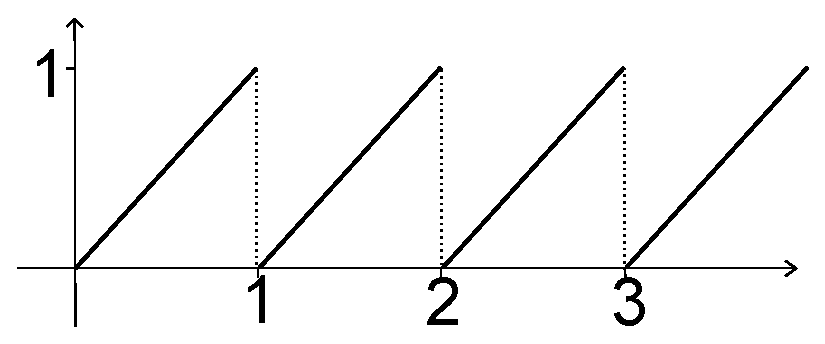
\includegraphics[width=2.5in]{11-laplaceII/sawtooth1.eps}
\end{center}


\ap A mass of $3 \ kg$ is attached to the end of a spring with spring constant $k=48 \frac{N}{m}$, and there is no damping.  The mass is initially at rest with no outside forces acting on the spring-mass system (including no gravity).  At time $t=4$ a hammer strikes the mass with $1 N \cdot s$ of impulse in the direction which stretches the spring.  Model this as a differential equation with a delta function, solve it, and graph the resulting solution.



\ap The delta function $\delta_a(t)$ can be thought of in some sense as a limit of the functions $\frac{1}{h} \left( \mathcal{U}_a(t)-\mathcal{U}_{a+h} (t) \right)$ as $h \searrow 0$. Illustrate this by {\bf (a)} finding a function $y$ which solves $\ddot{y} = \frac{1}{h} \left( \mathcal{U}_a(t)-\mathcal{U}_{a+h} (t) \right)$ and writing it in piecewise notation, {\bf (b)} taking the limit of the result of part (a) as $h \searrow 0$, and {\bf (c)} comparing the result of (b) with the solution of $\ddot{y} = \delta_a(t)$.

\ap The problem above suggests that the delta function $\delta_a$ can be thought of as a derivative of a unit step function $\mathcal{U}_a$.  Make this explicit by calculating the value of $\int_{-\infty}^t \delta_a(x) \ dx$ for $t \neq a$ and explaining how the results suggests a relationship between $\delta_a$ and $\mathcal{U}_a$.

\ap Find the Fourier Transform of the translated delta function, $F[\delta_a(t)]$.  {\it (Refer to the definition of the Fourier Transform given in Problem 10.4, and use the defining properties of the delta function.)}

\ap Express the function $f(t) = \frac{\sqrt{t^2}+t}{2t}$ in terms of unit step functions.  {\it (Hint: you can guess the answer by graphing $f(t)$ first; once you know what the answer should be, explain how to see this result from the formula itself.)} This question illustrates the fact that we don't really need to resort to piecewise notation to define step functions -- that just happens to be an easier way to do it.


\end{multicols}

 




 % LAPLACE DISCONTINUOUS DRIVING FUNCTIONS

\chapter{Representation Formulas and Convolutions}

\setcounter{example}{1}
\setcounter{exercise}{1}

{\begin{center}
\psframebox[style=profibox]{\begin{minipage}{4in}
{\bf Prototype Question:} 
Find a formula for the solution of $\ddot{y} - 4 y = f(t)$, $y(0)=0)$, $\dot{y}(0)=0$ which can be evaluated to any desired accuracy for any given function $f(t)$.
\end{minipage}
}
\end{center}





In this section, we will write down several integral formulas for solutions of ODE.  These formulas are especially useful when it is difficult or impossible to write down closed form anti-derivatives.

Let us begin by considering the general first-order linear equation in standard form:
\[ \frac{dy}{dx}+p(x)y=q(x).\]
Suppose we seek a solution that satisfies the initial condition $y(x_0)=y_0$.  On a domain $I$ containing $x_0$ and where $p(x)$ and $q(x)$ are continuous, we would normally introduce any integrating factor of the form $\exp \left( \int p(x)dx \right)$.  However, let us now specify a particular anti-derivative as the argument of the exponential function (by taking advantage of the Fundamental Theorem of Calculus): we will use the integrating factor $\mu(x)=\exp \left( \int_{x_0}^x p(s)ds \right)$.
\[ \frac{d}{dx}\left[ \exp \left(\int_{x_0}^x p(s) ds \right) y \right] = q(x)\exp \left(\int_{x_0}^x p(s) ds \right).\]
And again, when we anti-differentiate both sides of this equation, we will use a particular anti-derivative on the right side:
\[ \exp \left( \int_{x_0}^x p(s) ds \right) y = C+\int_{x_0}^x q(t) \exp \left(\int_{x_0}^t p(s) ds \right)  dt. \]
(Note the presence of the constant of integration $C$ on the right side.)  
If we insert the initial condition at this point, notice that both definite integrals will be zero (since the upper and lower limits of integration will be identical), and we can see that $y_0=C$, so now we have
\[ \exp \left( \int_{x_0}^x p(s) ds \right) y = y_0+\int_{x_0}^x q(t) \exp \left(\int_{x_0}^t p(s) ds \right)  dt. \]
Isolating $y$ yields


{\begin{center}
\psframebox[style=formulabox]{\begin{minipage}{4.5in}
{\bf {\color{OliveGreen} Representation Formula for First-Order Linear Initial Value Problems \normalcolor}}

If $p(x)$ and $q(x)$ are continuous on an open interval $I$ containing $x_0$, then the unique solution of $y'+p(x)y=q(x)$ on $I$ is given by 
\[ y = \exp \left( -\int_{x_0}^x p(s) ds \right)  \left(y_0+\int_{x_0}^x q(t) \exp \left(\int_{x_0}^t p(s) ds \right) dt \right). \]
\end{minipage}
}
\end{center}



This is a representation formula that can be used for any first-order linear IVP in standard form.  The integrals are guaranteed to be defined on any domain where $p$ and $q$ are both continuous.  Even when we cannot write down an anti-derivative for the functions $p$ and $q$, we can often still write down approximate values of $y(x)$ by using a numerical method to approximate the integrals (such as the Trapezoid Rule, Simpson's Rule or another algorithm run by a calculator or computer.

\example Suppose $y$ satisfies the initial value problem $y'+2xy=1, \ y(0)=2$.  Find the approximate value of $y(1)$.

In theory the method of integrating factors will apply here, but we will run into some difficulty if we try actually calculate the exact solution because we will end up trying to anti-differentiate $e^{(x^2)}$, and there is no closed-form anti-derivative for this function.  However, we can apply the representation formula above (which is really just the method of integrating factors anyway) with $p(x)=2x$ and $q(x)=1$ to get
\begin{align*}
y(x) & = \exp \left( -\int_0^x 2s \ ds \right) \left( 2 + \int_0^x 1 \exp \left(\int_0^t 2s \ ds \right) dt \right) \\
& = e^{-(x^2)} \left( 2 + \int_0^x e^{(t^2)} \ dt \right)
\end{align*}
In particular,
\[ y(1) = e^{-1} \left( 2 + \int_0^1 e^{(t^2)} \ dt \right).\]
The integral on the right side can be calculated to any desired accuracy.  Simpson's Rule with $n=10$ subdivisions gives us $\int_0^1 e^{(t^2)} dt \approx 1.46268$.  Therefore $y(1) \approx 1.27385.$  (Careful use of the error estimate for Simpson's rule and careful rounding would allow us to conclude that the accuracy of this answer is better than  $10^{-4}$.)
\qed





\begin{exe} Use the above representation formula to write down a solution to $y'+xy=1$, $y(0)=1$.  Then give an approximate value of $y(2)$ by using a numerical method or computer to evaluate the definite integrals involved.
\end{exe}

Another representation formula can be obtained using the method of Laplace Transforms.  The key idea necessary is an operation on functions which is called convolution, so we must take a brief excursion to define this operation and examine some of its properties.

In pre-calculus we learn about several operations that combine functions.  The first few operations we explore are based on arithmetic: addition, subtraction, multiplication and division of functions.  Then we introduce a new operation that is different from what one has studied before: composition of functions.  Now will explore yet another way of combining functions which is of particular interest when working with Laplace Transforms.  This operation is defined in terms of definite integrals.

The 
	\index{convolution}%
	{\bf convolution} of two integrable functions $f$ and $g$ defined on $[0,\infty)$ is written as $f * g$ and is defined by the formula
\[ f*g (t) = \int_0^t f(\tau) g(t-\tau) \ d\tau.\]

\example Let $f(t)=t$ and $g(t)=e^t$.  Compute $f*g$.
\begin{align*}
f*g(t) & = \int_0^t f(\tau) g(t-\tau) \ d\tau \\
& = \int_0^t \tau e^{t-\tau} \ d\tau \\
& = e^t \int_0^t \tau e^{-\tau} \ d\tau \\
& = e^t \left( -\tau e^{-\tau} + \int e^{-\tau} \ d\tau \right)_0^t \\
& = e^t \left( -\tau e^{-\tau} -e^{-\tau} \right)_0^t \\
& = e^t(-t e^{-t} - e^{-t}+0+1) \\
& = -t-1+e^t.
\end{align*}
\qed

The first fact we will prove about convolution is that it is commutative: $f*g=g*f$.  Indeed,
\begin{align*}
f*g & = \int_{\tau=0}^{\tau=t} f(\tau)g(t-\tau) \ d\tau \\
& = -\int_{u=t}^{u=0} f(t-u)g(u) \ du \ \ \ \mbox{(substituting $u=t-\tau$)} \\
& = \int_{u=0}^{u=t}g(u)f(t-u) \ du \\
& = g*f.
\end{align*}
Therefore we need not specify the order of the two functions in a convolution.  

\begin{exe} 
Prove (by giving a counterexample) that the composition of functions $f \circ g$, defined by $(f \circ g)(x) = f(g(x))$, is not a commutative operation.
\end{exe}


\begin{exe} 
Find the convolution of the functions $t$ and $t^2$.
\end{exe}


Next, we examine what happens when we take the Laplace Transform of a convolution.
\begin{align*}
L[f*g] & = \int_0^\infty f*g(t) e^{-st} \ dt \\
& = \lim_{T \rightarrow \infty} \int_0^T \int_0^t f(\tau) g(t-\tau) e^{-st} \ d\tau \ dt \\
& = \lim_{T \rightarrow \infty} \int_0^T \int_\tau^T f(\tau) g(t-\tau) e^{-st} \ dt \ d\tau \ \ \ \ \ (*) \\
& = \lim_{T \rightarrow \infty} \int_0^T \int_0^{T-\tau} f(\tau)g(u)e^{-s(u+\tau)} \ du \ d\tau \\
& = \int_0^\infty \int_0^\infty f(\tau)g(u)e^{-s\tau}e^{-su} \ du \ d\tau \\
& = \left( \int_0^\infty f(\tau) e^{-s\tau} \ d\tau \right) \left( \int_0^\infty g(u) e^{-su} \ du \right) \\
& = (L[f])(L[g]).
\end{align*} 
In the line marked (*) we changed the order of integration, and the following figure illustrates how we obtained the new limits of integration:
\begin{center}
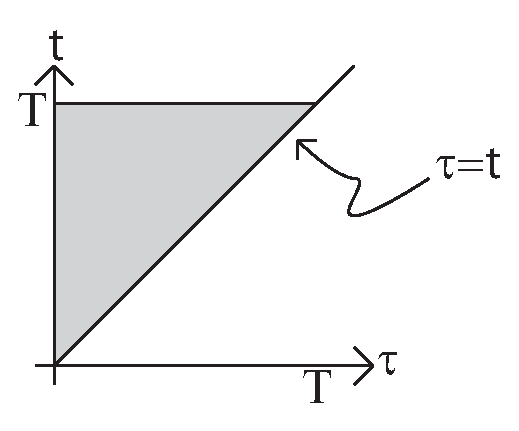
\includegraphics[width=2.5in]{12-representationformulas/convolutionfubini.eps}
\end{center}
What this result shows is that the Laplace Transform of a convolution of two functions is just the product of their Laplace Transforms.  This fact is valuable to us because it helps us to find more inverse transforms.


{\begin{center}
\psframebox[style=formulabox]{\begin{minipage}{4.5in}
{\bf {\color{OliveGreen} Laplace Transform of a Convolution \normalcolor}}
\index{convolution, Laplace transform of}

\[ L[f*g] = L[f]L[g].\]
Equivalently,
\[ L^{-1}[F(s)G(s)] = L^{-1}[F(s)] * L^{-1}[G(s)]. \]
\end{minipage}
}
\end{center}


\example The inverse Laplace Transform of $\frac{1}{(s-a)^2}$ is $te^{at}$ since
\begin{align*}
L^{-1} \left[ \frac{1}{s-a} \ \frac{1}{s-a} \right] & = L^{-1} \left[ \frac{1}{s-a}\right] * L^{-1} \left[ \frac{1}{s-a} \right] \\
& = e^{at} * e^{at} \\
& = \int_0^t e^{a\tau} e^{a(t-\tau)} \ d\tau \\
& = \int_0^t e^{at} \ d\tau \\
& = \left. \tau e^{at} \right|_0^t \\
& = te^{at}.
\end{align*}
\qed

\begin{exe}
Use the result of Example 3 above to solve the IVP $y''+10y'+25y=0, \ y(0)=1, \ y'(0)=2$ via Laplace Transforms.
\end{exe}

\begin{exe} 
Find $L^{-1} \left[ \frac{1}{s(s-1)} \right]$ two ways: (a) using convolutions and (b) using partial fractions.
\end{exe}





Now we have the necessary tool to develop more representation formulas.  

\example Find a formula for the solution of the initial value problem $\dot{y}+2y=f(t)$,  $y(0)=0$.  

Taking the Laplace Transform of each side of the differential equation produces
\[ L[\dot{y}+2y] = L[f],\]
so that
\[ s L[y]-y(0)+2L[y]=L[f],\]
and using the initial condition then isolating $L[y]$ yields
\[ L[y] = L[f]\frac{1}{s-1}.\]
If we know what $L[f]$ is, we might be able to evaluate this by hand, but only if we are able to look up the necessary inverse transforms in a table.  However, that is not necessary, because we come to this battle armed with convolutions!  Recall that $L[f*g]=L[f]L[g]$, and inverting that rule here with $g=L^{-1} \left[ \frac{1}{s-1} \right] = e^t$ gives us
\[ y = f(t) *e^t,\]
or
\[ y = \int_0^t f(\tau) e^{t-\tau} \ d\tau.\]
\qed

This formula can be applied even if we do not know the Laplace Transform of $f$.  For example, if $f(t)=\tan(t)$, and we want to know $y(0.5)$, then
\[ y(0.5) = \int_0^{0.5} \tan(\tau) e^{0.5 - \tau} \ d\tau = 0.155.\]
This approach gives us a numerical approximation, just like a technique such as Euler's Method would.  The advantage here is that we can obtain any desired accuracy provided we know how to approximate the necessary integral within the prescribed level of error.

\begin{exe}
Use Laplace Transforms and convolution to find an integral representation formula for $y(t)$ where $y$ satisfies the initial value problem $\dot{y} + 4y = \sec(t)$, $y(0)=0$, and use it to find an approximate value of $y(0.2)$.
\end{exe}

\begin{exe}
Use Laplace Transforms and convolution to find an integral representation formula for $y(t)$ where $y$  satisfies the initial value problem $\ddot{y}+4y = \cot(t)$, $y(0)=0$, $\dot{y}(0)=0$, and use it to find an approximate value of $y(0.3)$.
\end{exe}


\begin{exe}
Use Laplace Transforms and convolution to find an integral representation formula for $y(t)$ where $y$  satisfies the initial value problem $\ddot{y}-4\dot{y}+3y = e^{(t^2)}$, $y(0)=1$, $\dot{y}(0)=0$, and use it to find an approximate value of $y(0.2)$.
\end{exe}



%%% Cut below here for the book form.
%
%\newpage
%\begin{center} {\LARGE Problems} \end{center}
%
%\setcounter{problem}{1}




\newpage
\begin{center} {\LARGE Additional Exercises} \end{center}

\bigskip
\begin{multicols}{2}
\begin{instructions}
Write down an integral representation formula for the solution of the given initial value problem.  The use a graphing calculator or computer to evaluate the formula and approximate the value of $y(x_1)$.
\end{instructions}

\smallskip
\ap $y'+x^2y=1, \ y(0)=0, \ x_1 = 2$

\ap $y' + \sin(x) y = x, \ y(0)=0, \ x_1 = 1$

\ap $y' + \frac{y}{x} = e^{(x^4)}, \ y(0)=1, \ x_1 = 2$

\ap $y' - xy = x^2, \ y(0)=2, \ x_1 = 1$


\begin{instructions}
Calculate the given convolution of functions.
\end{instructions}

\smallskip
\ap $t^2 * t^2$

\ap $e^t * e^{2t}$

\ap $e^t * sin(t)$

\ap $cos(t) * cos(t)$


\begin{instructions} Use convolution to calculate the given inverse Laplace transform.
\end{instructions}

\smallskip
\ap $L^{-1} \left[ \frac{1}{(s-1)(s+1)} \right]$

\ap $L^{-1} \left[ \frac{1}{s(s+2)} \right]$

\ap $L^{-1} \left[ \frac{1}{s(s^2+1)} \right]$

\ap $L^{-1} \left[ \frac{1}{s^2(s^2+1)} \right]$

\begin{instructions} Use convolution to find an integral representation formula for the solution of the given initial value problem.
\end{instructions}

\smallskip
\ap $\ddot{y} = e^{(t^2)}, \ y(0)=0, \ \dot{y}(0)=0$

\ap $\ddot{y} + y = \tan(t), \ y(0)=0, \ \dot{y}(0)=0$

\ap $\ddot{y} - y = \cos(t^3), \ y(0)=0, \ \dot{y}(0)=0$

\ap $\ddot{y} -3\dot{y} + 2y = \sin(t^2), \ y(0)=0, \ \dot{y}(0)=0$


\smallskip
\hrule


\smallskip
\ap Use the method of integrating factors to find an integral representation formula for the solution of the following initial value problem with $b \neq 0$, and simplify your answer as much as possible:
\[ \dot{y}+by=f(t), \ y(0)=y_0.\]

\ap Use Laplace Transforms to find an integral representation formula for the solution of the following initial value problem with $b \neq 0$:
\[ \dot{y}+by=f(t), \ y(0)=y_0.\]

\ap Use Laplace Transforms to find an integral representation formula for the solution of the following initial value problem with $b \neq 0$:
\[ \ddot{y}+2b\dot{y}+b^2=f(t), \ y(0)=y_0, \dot{y}(0)=v_0.\]

\ap Use an integral representation formula to solve $\ddot{y}-y=f(t)$ with the initial conditions $y(0)=0$ and $\dot{y}(0)=0$.  Then let $f(t)=\ln(t-1)$, and estimate the value of $y(1)$ by evaluating the necessary definite integrals using Simpson's Rule.  Give an answer with an error less than $10^{-5}$.


\end{multicols}
 % REPRESENTATION FORMULAS AND CONVOLUTIONS 

\part{Systems of ODE}

\input{13-systems/systems.chapter} % INTRO TO SYSTEMS

\input{14-2x2systems/linearsystems.chapter} % INTRO TO SYSTEMS






%%								APPENDICES
\appendix
\setcounter{chapter}{0}

\input{A1-separationofvariables/separationofvariables.chapter} % SEPARATION OF VARIABLES

\appendix
\setcounter{chapter}{1}

\documentclass[12pt,letterpaper,twoside]{amsart}
\usepackage[latin1]{inputenc}
\usepackage{amsmath}
\usepackage{amsfonts}
\usepackage{graphicx}
\usepackage{amssymb}
\usepackage{multicol}
\usepackage{ulem}
\newcounter{example}
\newcounter{exercise}
\newcounter{problem}
\newtheorem{theorem}{Theorem}
\newcommand{\example}{\bigskip \noindent {\large {\sc Example \arabic{example}:}} \addtocounter{example}{1}}
\newcommand{\exercise}{\bigskip \noindent {\large {\sc Exercise \arabic{exercise}:}} \addtocounter{exercise}{1}}
\newcommand{\problem}{\bigskip \noindent {\large {\sc Problem \arabic{problem}:}} \addtocounter{problem}{1}}
\newcommand{\tech}{\marginpar{\vskip 10mm \begin{center}\includegraphics[width=0.25in]{calculatorimagesmall.eps} \end{center}}}
\newcommand{\solution}{\medskip \noindent {\bf Solution: }}
\newcommand{\R}{\mathbb{R}}





\begin{document}

\sffamily

%%%%  switch the commenting on this line and the next \chapter{Introduction}
\begin{center} {\LARGE Complex Numbers} \end{center}

\setcounter{example}{1}
\setcounter{exercise}{1}

When we solve characteristic equations, we are often faced with complex numbers.  For example, the solutions of a quadratic equation $ax^2+bx+c=0$ are given by the quadratic formula
\[ x = \frac{-b \pm \sqrt{b^2-4ac}}{2a},\]
and if the discriminant $b^2-4ac$ is negative, then we are looking at square roots of negative numbers, so the roots of the original equation are complex numbers -- these are numbers which can be written in the form
\[ z = \alpha + \beta i,\]
where $\alpha$ and $\beta$ are both real, and $i$ satisfies $i^2=-1$.  If $z=\alpha + \beta i$ in this way, then we call $\alpha$ the {\bf real part} of $z$, and we call $\beta$ the {\bf imaginary part}.

We can usually understand the arithmetic operations on complex numbers by writing numbers in terms of their real and imaginary parts.

\example Let $z=1+3i$ and $w=3-2i$.  Then:
\begin{itemize}
\item $z+w = (1+3i)+(3-2i)=(1+3)+(3-2)i=4+i$
\item $zw = (1+3i)(3-2i)=(1)(3)+(3i)(3)+(1)(-2i)+(3i)(-2i)=3-2i+3i-6i^2=3-2i+3i-6(-1)=9+i$
\end{itemize}

\exercise Let $u=2+4i$ and $v=1-2i$.  Find $2u+3v$ and $2uv$.

The {\bf complex conjugate} of $z=\alpha + \beta i$ is the complex number $\overline{z}=\alpha - \beta i$.  For example, $\overline{1+3i}=1-3i$.  

\exercise prove that for any complex number $z$, the product $z \cdot \overline{z}$ is a real number.

\medskip
The conjugate is thus useful for simplifying division with complex numbers:

\example Let $z=1+2i$ and $w=2-4i$.  Then
\begin{align*}
\frac{z}{w} & = \frac{1+2i}{2-4i} \\
& = \frac{(1+2i)}{(2-4i)} \frac{(2+4i)}{(2+4i)} \\
& = \frac{2+4i+4i+8i^2}{4-16i^2} \\
& = \frac{-6+8i}{20} \\
& = -\frac{3}{10}+\frac{2}{5}i.
\end{align*}

\exercise Let $u=2+4i$ and $v=1-i$.  Simplify the expressions $\frac{u}{v}$ and $\frac{v}{u}$.  Write the answers in the form $\alpha + \beta i$.

\medskip
In the study of ordinary differential equations, we will often see complex numbers arise in exponential functions. Therefore we now turn our attention to finding a better understanding of exponentials.

First of all, we need to say what we mean by $e^z$ when $z$ is complex.  To answer this, we turn to the power series representation of the exponential function:
\[ e^z = \sum_{n=0}^\infty \frac{z^n}{n!}.\]
(Here, we use the standard convention when working with power series that $0^0=1$.)  This series has an infinite radius of convergence and therefore converges for all complex numbers $z$.

To work with a complex exponent, we usually write it in terms of its real and imaginary parts, and then use a law of exponents to separate these:
\[ e^z = e^{\alpha + \beta i} = e^\alpha e^{\beta i}.\]
Therefore it will be profitable for us if we now focus our attention on expressions of the form $e^{\beta i}$, and that's where the power series representation becomes helpful:
\begin{align*}
e^{\beta i} & = \sum_{n=0}^\infty \frac{(\beta i)^n}{n!} \\
& = \sum_{n=0}^\infty \frac{\beta^n i^n}{n!} \\
& = \sum_{n=0, \ n \ even}^\infty \frac{\beta^n i^n}{n!} + \sum_{n=0, \ n \ odd}^\infty \frac{\beta^n i^n}{n!} \\
& = \sum_{n=0}^\infty \frac{\beta^{2n}i^{2n}}{(2n)!}+\sum_{n=0}^\infty \frac{\beta^{2n+1}i^{2n+1}}{(2n+1)!} \\
& = \sum_{n=0}^\infty \frac{\beta^{2n}(-1)^n}{(2n)!}+\sum_{n=0}^\infty \frac{\beta^{2n+1}i(-1)^n}{(2n+1)!} \\
& = \cos(\beta)+i\sin(\beta).
\end{align*}
Combining this with the previous result gives us:
\begin{center}
\fbox{
\begin{minipage}{2in}
\[ e^{\alpha + \beta i} = e^\alpha (\cos(\beta)+i\sin(\beta))\]
\end{minipage}
}
\end{center}

Note that in the calculation above, we made use of the power series for sine and cosine:
\[ \sin(z)=\sum_{n=0}^\infty \frac{z^{2n+1}(-1)^n}{(2n+1)!} \ \ \ \mbox{and} \ \ \ \cos(z) = \sum_{n=0}^\infty \frac{z^{2n} (-1)^n}{(2n)!}\]
These series also allow us to define sine and cosine for complex arguments, and this will be explored briefly in the problem set.

\exercise Find the values of $e^{\pi i}$, $e^{2\pi i}$ and $e^{2+\pi i/4}$.


\bigskip

%% Cut below here for the book form.

\begin{center} {\LARGE Problems} \end{center}

\setcounter{problem}{1}

\problem Prove that, if the solutions of the quadratic equation $ax^2+bx+c=0$ are complex numbers, and if the coefficients $a$, $b$ and $c$ are all real numbers, then the solutions are complex conjugates of one another.

\problem Prove that $\sin(z)=\frac{e^{-iz}-e^{iz}}{2}$.  Use this to evaluate $\sin(i)$.

\problem Find a representation formula for $\cos(z)$ (similar to the one for sine above) and use it to evaluate $\cos(2i)$.





\end{document} % COMPLEX NUMBERS

\documentclass[12pt,letterpaper,twoside]{amsart}
\usepackage[latin1]{inputenc}
\usepackage{amsmath}
\usepackage{amsfonts}
\usepackage{graphicx}
\usepackage{amssymb}
\usepackage{multicol}
\usepackage{ulem}
\newcounter{example}
\newcounter{exercise}
\newcounter{problem}
\newcommand{\example}{\bigskip \noindent {\large {\sc Example \arabic{example}:}} \addtocounter{example}{1}}
\newcommand{\exercise}{\bigskip \noindent {\large {\sc Exercise \arabic{exercise}:}} \addtocounter{exercise}{1}}
\newcommand{\problem}{\bigskip \noindent {\large {\sc Problem \arabic{problem}:}} \addtocounter{problem}{1}}
\newcommand{\tech}{\marginpar{\vskip 10mm \begin{center}\includegraphics[width=0.25in]{calculatorimagesmall.eps} \end{center}}}
\newcommand{\solution}{\medskip \noindent {\bf Solution: }}
\newcommand{\R}{\mathbb{R}}





\begin{document}

\sffamily

%%%%  switch the commenting on this line and the next \chapter{Introduction}
\begin{center} {\LARGE Reduction of Order} \end{center}

\setcounter{example}{1}
\setcounter{exercise}{1}

With this chapter we begin our study of second order ODE.  Sometimes it is easy to find one solution of a differential equation, and reduction of order con sometimes provide us with a way of using that one solution to find a formula for the general solution.

\example Consider the second order differential equation $\ddot{y}-y=0$.  We observe that the function $y_1(t)=e^t$ is a solution on the interval $\mathbb{R}$, and that this solution is non-zero for all $t \in \mathbb{R}$.  If $y(t)$ is {\it any} solution of the ODE, let $u(t)$ be defined by $u(t)=\frac{y(t)}{y_1(t)}$, or $y=uy_1$.  We substitute this into the ODE to see that
\begin{align*}
0 & = \ddot{y}-y \\
& = \frac{d^2}{dt^2}\left[ ue^t \right] - (ue^t)\\
& = (\ddot{u}e^t + 2\dot{u}e^t + ue^t)-(ue^t) \\
& = \ddot{u}e^t+2\dot{u}e^t.
\end{align*}
Dividing by $e^t$, which is never zero, gives us the following differential equation for $u$:
\[ \ddot{u}+2\dot{u}=0.\]
Make the substitution $v=\dot{u}$ to obtain
\[ \dot{v}+2v=0.\]
This equation can be solved using the method of integrating factors (the integrating factor is $e^{2t}$):
\begin{align*}
\frac{d}{dt} \left[ e^{2t} v \right] & = 0 \\
e^{2t} v & = C \\
v & = Ce^{-2t}
\end{align*}
Integrating this shows that $u=Ce^{-2t}+D$, and inserting this into the equation $y=uy_1$ we see that
\[ y(t)=(Ce^{-2t}+D)e^t = Ce^{-t}+De^{t}\]
is the general solution of the ODE.
\qed

The general process is:
\begin{itemize}
\item Find a solution $y_1$ of the ODE;
\item set $y=uy_1$, and apply this substitution for $y$ in the ODE;
\item simplify to find a differential equation for $u$;
\item find a general solution for $u$;
\item the product $y=uy_1$ gives the general solution for the ODE on the set where $y_1 \neq 0$.
\end{itemize}

The last point is am important one: because we define $u$ by $u=\frac{y}{y_1}$, this process is only guaranteed to give a formula for a general solution on the set where $y_1 \neq 0$.  One might get lucky and obtain a general solution on a larger domain, but there is no guarantee that will happen in general.

\exercise Verify that $y_1(x)=e^{-x}$ is a solution of the differential equation $y''+3y'+2y=0$.  Then use reduction of order to find a general solution of this ODE defined on $\mathbb{R}$.

\exercise Verify that $y_1(x)=e^{2x}$ is a solution of $y''-2y'=0$.  The use reduction of order to find a general solution on $\mathbb{R}$.

\exercise Verify that $y_1(t)=t$ is a solution of the ODE $t^2 \ddot{y} +2t \dot{y} -2y=0$.  Then use reduction of order to find the general solution of this ODE defined on the interval $(0,\infty)$.

\exercise Verify that $y_1(t)=\sin(2t)$ is a solution of the ode $\ddot{y}+4y=0$.  Then use reduction of order to find a general solution on $\mathbb{R}$.  {\it (Note: Because $y_1(t)=0$ for $t=\frac{k\pi}{2}$, the method only guarantees a solution on an interval of the form $\left( \frac{k\pi}{2},\frac{(k+1)\pi}{2}\right)$; therefore you will need to verify directly that the formula you obtain is a solution on $\mathbb{R}$.)}

Now we will explore the theory of this method -- that is to say, we will discuss why it works.

Begin with an ODE of the form
\[ a(x)y''+b(x)y'+c(x)y=0,\]
and a function $y_1(x)$ which is a solution of this equation.  Let $I$ be an open interval where $y_1 \neq 0$.  Then if $y(x)$ is {\it any} solution of this ODE on $I$, we can define $u=\frac{y}{y_1}$ on $I$; thus $y=uy_1$.  The product rule gives us $y'=u'y_1 +uy_1'$ and $y''=u''y_1 + 2u'y_1'+uy_1''$.  Inserting these into the ODE yields
\begin{align*}
0 = &  a(x)y''+b(x)y'+c(x)y \\
& = a(x)\left(u''y_1 + 2u'y_1'+uy_1''\right)+b(x)\left(u'y_1 +uy_1'\right)+c(x)(uy_1) \\
& = a(x) y_1 u'' + (2a(x)y_1'+b(x)y_1)u'+(a(x)y_1''+b(x)y_1'+c(x)y_1)u,
\end{align*}
and the last term in the last line is zero on $I$ since $y_1$ solve the ODE there.  we are thus left with
\[ a(x)y_1u''+(2a(x)y_1'+b(x)y_1)u'=0.\]
If we make the subsitution $v=u'$, we get
\[ a(x) y_1(x)v'+(2a(x)y_1'(x)+b(x)y_1(x)v=0.\]
This is a first order equation that can typically be solved to find a general formula for $v$, and integrating that solution gives us a general formula for $u$; inserting that formula for $u$ into the equation $y=uy_1$ gives us a general formula for $y$ on $I$.

It is because of the fact we always obtain an equation of the form $\tilde{a}(x)u''+\tilde{b}(x)u'=0$, which can be reduced to a first order equation via the substitution $v=u'$, that this method gets it name.



%% Cut below here for the book form.

\begin{center} {\LARGE Problems} \end{center}

\setcounter{problem}{1}

\problem Verify that the function $y_1(t) = e^t$ is a solution of the third order ODE $y'''-y=0$.  Then let $y$ be any other solution of the ODE, and use reduction of order to show that $y=ue^x$, where $u$ is a solution of the ODE $u'''+3u''+3u'=0$.  {\it (Do not try to solve this ODE.)}

\problem Find a power function $y_1(x)=x^n$ that solves the differential equation $x^2y''-3xy'+4y=0$.  Then use reduction of order to find a general solution on the interval $(0,\infty)$.

\problem Find a power function $y_1(x)=x^n$ that solves the differential equation $x^2y''-7xy'-6y=0$.  Then use reduction of order to find a general solution on the interval $(0,\infty)$.

\problem Consider the ODE  $y''-2\alpha y'+a^2 y=0$, where $\alpha$ is a constant.  {\bf (a)} Find a value of $r$ such that $y_1(x)=e^{rx}$ is a solution of this ODE.  {\it (Hint: Do this by substituting $e^{rx}$ for $y$ and solving for $r$.)} {\bf (b)} Use the solution you found in part (a) and reduction of order to find a general solution of the ODE.

\problem Consider the ODE $y''-(\alpha+\beta)y'+\alpha \beta y=0$, where $\alpha, \ \beta$ are constants and $\alpha \neq \beta$.  {\bf (a)} Prove that the only values of $r$ such that $y_1(x)=e^{rx}$ solves the ODE are $r=\alpha$ and $r=\beta$.  {\bf (b)} Use the solution $y_1(x)=e^{\alpha x}$ and reduction of order to find the general solution of the ODE. Simplify your solution.





\end{document} % REDUCTION OF ORDER


%% WHY DO I HAVE TO FORCE CORRECT NUMBERING OF THE APPEDICES?????????


\documentclass[12pt,letterpaper,twoside]{amsart}
\usepackage[latin1]{inputenc}
\usepackage{amsmath}
\usepackage{amsfonts}
\usepackage{graphicx}
\usepackage{amssymb}
\usepackage{multicol}
\usepackage{ulem}
\newcounter{example}
\newcounter{exercise}
\newcounter{problem}
\newcommand{\example}{\bigskip \noindent {\large {\sc Example \arabic{example}:}} \addtocounter{example}{1}}
\newcommand{\exercise}{\bigskip \noindent {\large {\sc Exercise \arabic{exercise}:}} \addtocounter{exercise}{1}}
\newcommand{\problem}{\bigskip \noindent {\large {\sc Problem \arabic{problem}:}} \addtocounter{problem}{1}}
\newcommand{\tech}{\marginpar{\vskip 10mm \begin{center}\includegraphics[width=0.25in]{calculatorimagesmall.eps} \end{center}}}
\newcommand{\solution}{\medskip \noindent {\bf Solution: }}
\newcommand{\R}{\mathbb{R}}
\usepackage{newcent}
\newenvironment{exe}{\medskip \small \exercise}{\normalsize \medskip}

\newcommand{\I}{\left[ \begin{matrix} 1 & 0 \\ 0 & 1 \end{matrix} \right]}
\newcommand{\startmatrix}{\left[ \begin{matrix}}
\newcommand{\finishmatrix}{\end{matrix} \right]}

\begin{document}


%%%%  switch the commenting on this line and the next \chapter{Introduction}
\begin{center} {\LARGE Matrix Algebra} \end{center}

\setcounter{example}{1}
\setcounter{exercise}{1}

A {\bf matrix} is a rectangular array of numbers (real or complex), usually enclosed by large square brackets.  The {\bf dimension} of a matrix is $m \times n$, where $m$ is the number of rows (horizontal lines in the array) and $n$ is the number of columns (vertical lines in the array).

\example The matrix
\[ A = \left[ \begin{matrix} 2 & 3 & -9 \\ -1 & 0 & \frac{1}{5} \end{matrix} \right] \]
has two rows and three columns.  Therefore the dimension of $A$ is $2 \times 3$.
\qed

If a matrix has only one row or only one column, we call it a {\bf vector}.  If we wish to specify what the situation is, we can call it a {\bf row vector} (so that it is $1 \times n$) or a {\bf column vector} (so that it is $n \times 1$).

The values in each row and column of a matrix are called the {\bf entries} of the matrix.  We can specify an entry be stating the row and column in which it appears.  This is usually done using two subscripts attached to the symbol representing the matrix; the first subscript indicates the row, and the second subscript indicates the column.  For example, the entry in the $i^{th}$ row and $j^{th}$ column of a matrix $A$ is denoted by $A_{ij}$.  Two matrices of the same dimension are equal if and only if all their entries are equal.

\example Let 
\[ B = \left[ \begin{matrix} 2 & 4 \\ -1 & 0 \end{matrix} \right]. \]
The entry $B_{11}$ is the entry in the first rwo and first column, so $B_{11}=2$.  Also, $B_{12}$ is the entry in the first row and second column, so $B_{12}=4$.  Similarly, $B_{21}=-1$ and $B_{22}=0$.
\qed

If two matrices are of the same dimension, we can add and subtract one from another by adding or subtracting each corresponding entry.  Formally, we state this by saying that if $C=A+B$, then $C_{ij}=A_{ij}+B_{ij}$.  Also, if $D=A-B$, then $D_{ij}=A_{ij}-B_{ij}$.  We can also multiply a matrix by a scalar by distributing the multiplication to each entry in the matrix: if $E=cA$, then $E_{ij}=cA_{ij}$.  Note that for every scalar $c$, $cA=Ac$.

\example Let
\[ A= \left[ \begin{matrix} 1 & 3 \\ 0 & -2 \end{matrix} \right] \ \ \ \mbox{and} B \ \ \ = \left[ \begin{matrix} 1 & -4 \\ 1 & 3 \end{matrix} \right]. \]
Then
\[ A+B = \left[ \begin{matrix} 2 & -1 \\ 1 & 1 \end{matrix} \right] \ , \ \ \ A-B= \left[ \begin{matrix} 0 & 7 \\ -1 & -5 \end{matrix} \right] \ \ \ \mbox{and} \ \ \ 
3A = \left[ \begin{matrix} 3 & 9 \\ 0 & -6 \end{matrix} \right] \]
 \qed

We would also like to multiply matrices together, and it turns out that the useful way to define this is not the obvious way.  We will not simply multiply corresponding entries.  For application purposes, it is far more useful to define matrix multiplication as follows: if $A$ is an $m \times k$ matrix and $B$ is an $k \times n$ matrix, then the entries of the product matrix $AB$ are
\[ (AB)_{ij} = \sum_{l=1}^k A_{il}B_{lm}.\]
This operation is only defined when the number of columns of the first matrix matches the number of rows of the second matrix, and the result is a matrix that has the same number of rows as $A$ and the same number of columns as $B$.  That is to say, if $A$ is $m \times k$ and $B$ is $k \times n$, then $AB$ is $m \times n$.

\example Let 
 \[ A= \left[ \begin{matrix} 1 & 3 \\ 0 & 2 \end{matrix} \right] \ \ \ \mbox{and} \ \ \ B = \left[ \begin{matrix} 1 & 4 & 0 \\ 1 & 3 & 1 \\\end{matrix} \right]. \]
 Then
 \[ AB = \left[ \begin{matrix} (1 \cdot 1+3\cdot 1) & (1\cdot 4 +3\cdot 3) & (1 \cdot 0 + 3 \cdot 1)\\ (0\cdot 1 + 2\cdot 1) & (0 \cdot 4 + 2 \cdot 3) & (0 \cdot 0 + 2 \cdot 1) \end{matrix} \right] = \left[ \begin{matrix} 4 & 13 & 3 \\ 2 & 6 & 2 \end{matrix} \right],\]
but $BA$ is not defined.
\qed

\begin{exe} Let $A = \startmatrix 2 & 3 \\ 1 & -1 \finishmatrix$ and $B = \startmatrix 1 & -1 \\ 3 & 0 \finishmatrix$.  Calculate $AB$ and $BA$.
\end{exe}

The last exercise shows that matrix multiplication is not commutative: even if both multiplications $AB$ and $BA$ are defined,
\[ AB \neq BA \ \mbox{in general}.\]
(Both products could be equal, but usually that is not the case.)  On the other hand, matrix multiplication is distributive:
\[ A(B+C)=AB+AC,\]
provided the matrices have dimensions for which the additions and multiplications are all defined.  

The notation $I_n$ is used to denote an $n \times n$ {\bf identity matrix}.  It has entries of 1 along the main diagonal (from top left to bottom right) and the entries are zero everywhere else.  For example,
\[ I_2 = \left[ \begin{matrix} 1 & 0 \\ 0 & 1 \end{matrix} \right].\]
If the appropriate dimension is clear from context, we often omit the subscript and just write $I$.  For example, if $I$ is used to multiply a matrix $A$ on the left, as in the product $IA$, then the multiplication is only defined if the number of columns of $I$ matches the number of rows of $A$.  When this is defined, it turns out that $IA=A$ for every matrix $A$.

\begin{exe}
Let 
\[A=\left[ \begin{matrix} 2 & 4 \\ -1 & 0 \end{matrix} \right].\]
Verify that $IA=A$ and $AI=A$ by actually carrying out the matrix multiplications.
\end{exe}

One of the main reasons this definition of multiplication is useful is that it allows us to write a system of linear equations as a matrix equation.

\example Consider the following system of two linear equations in two unknowns:
\begin{align*} 3x-2y & = 4 \\ 2x+y & = 0 \end{align*}
These two scalar equalities can be written as a matrix equality:
\[ \left[ \begin{matrix} 3x-2y \\ 2x+y \end{matrix} \right] = \left[ \begin{matrix} 4 \\ 0 \end{matrix} \right].\]
But notice that the left side can be written as a product of matrices:
\[ \left[ \begin{matrix} 3 & -2 \\ 2 & 1 \end{matrix} \right] \left[ \begin{matrix} x \\ y \end{matrix} \right] = \left[ \begin{matrix} 4 \\ 0 \end{matrix} \right].\]
Thus if $A=\left[ \begin{matrix} 3 & -2 \\ 2 & 1 \end{matrix} \right]$, $X=\left[ \begin{matrix} x \\ y \end{matrix} \right]$ and $B=\left[ \begin{matrix} 4 \\ 0 \end{matrix} \right]$, then the system of equations above can represented by 
\[ AX=B.\]
\qed

When writing a system of linear equations as a matrix equation as in the last example, the matrix $A$ is called the {\bf coefficient matrix}.  In a course on linear algebra, students learn how to solve this equation for $X$ in a variety of ways.  If the coefficient matrix $A$ is a {\bf square matrix}, meaning that it has the same number of rows as columns, then it is sometimes possible to find an inverse matrix $A^{-1}$ such that $A^{-1}A=I$.  In such an instance, we would multiply both sides of the matrix equation to obtain
\[ A^{-1} A X = A^{-1} B,\]
or 
\[ IX = A^{-1}B,\]
which is the same as
\[ X = A^{-1}B.\]
If it is possible to solve the equation this way, then there must be exactly one solution for each matrix $B$.  (We will pursue this approach to solving equations a little in the problem set.)  This motivates the following question which we will pursue immediately: under what conditions on $A$ does the matrix equation $AX=B$ have exactly one solution for the unknown column vector $X$?

Let us write the general situation for a $2 \times 2$ matrix $A$:
\[ A = \left[ \begin{matrix} a & b \\ c & d \end{matrix} \right], \ X = \left[ \begin{matrix} x \\ y \end{matrix} \right]  \ \ \ \mbox{and} B = \left[ \begin{matrix} k \\ l \end{matrix} \right] .\]
The matrix equation $AX=B$ is equivalent to the system of scalar equations:
\begin{align*} ax+by = k \\ cx+dy=l \end{align*}
We can think of this system as a collection of lines in the $xy$-plane and the solution of this system as the point of intersection of those lines.  There will be infinitely many solutions if the lines are actually the same line, and there will be no solution if the lines are parallel.  There will be exactly one solution if the lines are not the same and not parallel.  Furthermore, we can assume that no row of $A$ can contain only zeros, otherwise there will be no solution when $B$ has a non-zero entry in the same row.

In the latter case, there are two situations to consider: either one line is vertical, or neither line is vertical.  (Both lines cannot be simultaneously vertical because we have assumed they are not parallel).  If $ax+by=k$ is vertical, then $b=0$ and $a \neq 0$; also, $d \neq 0$ since $cx+dy=l$ cannot be vertical; consequently 
\[ad-bc=ad-0c=ad \neq 0.\]
On the other hand, if $cx+dy=l$ is the vertical line, we have
\[ ad-bc = a0-bc =bc \neq 0\]
because $b\neq 0$ and $c \neq 0$.  Finally, if neither line is vertical, then their slopes are given by the ratios $\frac{-a}{b}$ and $\frac{-c}{d}$, and if the lines are not parallel, then these slopes are not equal:
\[ \frac{-a}{b} \neq \frac{-c}{d} \implies ad \neq bc \implies ad-bc \neq 0.\]
In every possible case we came to the conclusion $ad-bc \neq 0$.  If this condition fails, then the lines have the same slope, and therefore matrix equation $AX=B$ will either have infinitely many solutions or no solutions, depending on the choice of $B$.

\begin{exe} 
Prove that if $ad-bc=0$, then the matrix equation $AX=B$ with unknown column vector $X$ will have either no solution or infinitely many solutions, depending on the column vector $B$. Here, $A = \startmatrix a & b \\ c & d \finishmatrix$. {\it (Hint: Start by writing the matrix equation as a system of linear equations.  Multiply the first equation by $d$ and the second equation by $b$.  Solve the system by the elimination (or addition) method.  From this, deduce conditions on $B$.)}
\end{exe}

The point is that the quantity $ad-bc$ can be used to completely determine whether the matrix equation $AX=B$ has exactly one solution or not.  This quantity is called the {\bf determinant} of the matrix, and it is written as $\det(A)$:
\[ \det \left[ \begin{matrix} a & b \\ c & d \end{matrix} \right] =ad-bc.\]

\begin{exe}
Let $A = \left[ \begin{matrix} 2 & 0 \\ 1 & -1 \end{matrix} \right]$.  Calculate the determinant of $A$.
\end{exe}

Let us use $0$ to denote a zero-matrix or zero-vector (i.e. a matrix all of whose entries are zero).  The dimension of $0$ will be discernible from context.  Observe that the equation $AX=0$ always has a solution; $X=0$.  This is called the {\bf trivial solution} of the equation.  Many times will will want to know if there is a non-trivial solution.

\begin{exe} Find at least one non-trivial solution of $AX=0$, where $A = \left[ \begin{matrix} 2 & -1 \\ -4 & 2 \end{matrix} \right] $.
\end{exe}

We will also be interested in whether there are any non-trivial solutions of the equation
\[ AX=\lambda X.\]
Here, $\lambda$ is a scalar.  Again, note that the trivial solution $X=0$ always works.  If there is a non-trivial solution, it is called an {\bf eigenvector} for the matrix $A$, and $\lambda$ is called an associated {\bf eigenvalue}.

\begin{exe}
Let $A= \left[ \begin{matrix} 2 & 4 \\ 0 & 3 \end{matrix} \right]$.  Verify that $X=\left[ \begin{matrix} 1 \\ 0 \end{matrix} \right]$ is an eigenvector for $A$ with associated eigenvalue $\lambda = 2$.  Verify that the matrix $Y = \startmatrix 0 \\ 1 \finishmatrix$ is not an eigenvector for any possible eigenvalue.
\end{exe}

Next, we turn to the problem of finding eigenvalues and eigenvectors for a given matrix.

\begin{exe} 
Verify that the equation $AX=\lambda X$ is equivalent to $(A-\lambda I)X=0$.
\end{exe}

Because an eigenvector of $A$ is a non-trivial solution of $(A-\lambda I)X=0$, we know that there will be such a solution if and only if $\det(A-\lambda I)=0$.  For otherwise, if $\det(A-\lambda I) \neq 0$, then the equation $(A-\lambda I)X=0$ has exactly one solution, meaning that the trivial solution $X=0$ is the only one.  Therefore we can use the determinant of $A - \lambda I$ to find all the eigenvalues of a matrix. The equation $\det(A-\lambda I)=0$ is called the {\bf characteristic equation} for $A$.

\example Let $A=\left[ \begin{matrix} 2 & 4 \\ 0 & 3 \end{matrix} \right].$ Let us find all the eigenvalues of $A$.  For any eigenvalue $\lambda$, we will have
\begin{align*}
0 & = \det (A-\lambda I) \\
& = \det \left( \left[ \begin{matrix} 2 & 4 \\ 0 & 3 \end{matrix} \right] - \I \right) \\
& = \det \left[ \begin{matrix} 2-\lambda & 4 \\ 0 & 3-\lambda \end{matrix} \right] \\
& = (2-\lambda)(3-\lambda)-(4)(0) \\
& = (2-\lambda)(3-\lambda).
\end{align*}
The solutions of the characteristic equation $(2-\lambda)(3-\lambda)=0$ are $\lambda=2$ and $\lambda=3$, so these are the eigenvalues of $A$.
\qed

Once we know the eigenvalues, we can insert them for $\lambda$, and then finding eigenvectors to go with them is just a matter of solving a system of linear equations.

\example Let us find the eigenvalues and eigenvectors of $A = \left[ \begin{matrix} 11 & -5 \\ -18 & 24 \end{matrix} \right]$. The characteristic equation is
\begin{align*}
0 & = \det \left( \left[ \begin{matrix} 11 & -5 \\ -18 & 24 \end{matrix} \right] - \lambda \I \right) \\
& = \det \left[ \begin{matrix} 11-\lambda & -5 \\ -18 & 24-\lambda \end{matrix} \right] \\
& = (11-\lambda)(24-\lambda)-(-5)(-18) \\
& = \lambda^2 - 35 \lambda + 264 -90 \\
& = \lambda^2 -35 \lambda + 174.
\end{align*}
We can solve this equation using the quadratic formula:
\begin{align*}
\lambda & = \frac{35 \pm \sqrt{(-35)^2-4(1)(174}}{2(1)} \\
& = \frac{35 \pm \sqrt{529}}{2} \\
& = \frac{35 \pm 23}{2},
\end{align*}
so that $\lambda_1 = 29$ and $\lambda_2 = 6$ are the eigenvalues.

Next we identify the eigenvectors corresponding to each eigenvalue.  Using the eigenvalue $\lambda_1=29$ in the equation $A-\lambda I=0$ and writing the corresponding eigenvector as $\startmatrix a \\ b \finishmatrix$, we obtain
\[ \startmatrix -18 & -5 \\ -18 & -5 \finishmatrix  \startmatrix a \\ b \finishmatrix = \startmatrix 0 \\ 0 \finishmatrix \]
Both lines of this matrix equation correspond to the algebraic equation $-18a-5b=0$, which implies $b = -\frac{18a}{5}$.  Therefore, any matrix of the form $\startmatrix a \\ \frac{-18a}{5} \finishmatrix$ is an eigenvector corresponding to the eigenvalue $\lambda_1=29$.  This can also be stated by saying that any non-zero scalar multiple of $\startmatrix 1 \\ \frac{-18}{5} \finishmatrix$ is an eigenvector.

Turning to the eigenvalue $\lambda_2=6$, the matrix equation $(A-\lambda I)X=0$ can be written as
\[ \startmatrix 5 & -5 \\ -18 & 18 \finishmatrix \startmatrix c \\ d \finishmatrix = \startmatrix 0 \\ 0 \finishmatrix \]
and both lines of this matrix equation are algebraically equivalent to the scalar equation $c-d=0$, so that $c=d$.  Consequently, we see that non-zero vectors of the form $\startmatrix a \\ a \finishmatrix$ (equivalently, non-zero scalar multiples of $\startmatrix 1 \\ 1 \finishmatrix$) are eigenvectors corresponding to the eigenvalue $\lambda_2=6$.
\qed

\begin{exe}
Find the eigenvalues and corresponding eigenvectors for the matrix $A = \startmatrix 4 & 0 \\ 6 & -2 \finishmatrix$.
\end{exe}

\begin{exe}
Use the definition of eigenvalue and eigenvector to prove that, if $X$ is an eigenvector corresponding to the eigenvalue $\lambda$, then every non-zero scalar multiple of $X$ is also an eigenvector corresponding to $\lambda$.
\end{exe}

Eigenvalues and eigenvectors can also be complex, even if the entries of the original matrix are all real.

\example Let $A = \startmatrix 0 & 1 \\ 1 & 0 \finishmatrix$.  The characteristic equation is
\begin{align*}
0 & = \det \left( \startmatrix 0 & 1 \\ 1 & 0 \finishmatrix - \I \right) \\
& = \det \startmatrix -\lambda & 1 \\ -\lambda & 1 \finishmatrix \\
& = \lambda^2+1.
\end{align*}
The solutions of the equation $\lambda^2+1=0$ are $\lambda_1=i$ and $\lambda_2=-i$.  For the first case, the eigenvectors $\startmatrix a \\ b \finishmatrix$ satisfy
\[ \startmatrix -i & 1 \\ 1 & -i \finishmatrix \startmatrix a \\ b \finishmatrix = \startmatrix 0 \\ 0 \finishmatrix,\]
implying the scalar equation $-i a + b = 0$, so $b=ia$.  Thus the eigenvectors corresponding to $\lambda_1=i$ are the non-zero scalar multiples of $\startmatrix 1 \\ i \finishmatrix$.  Turning to the eigenvalue $\lambda_2=-i$, we have the matrix equation for the eigenvectors:
\[ \startmatrix i & 1 \\ 1 & i \finishmatrix \startmatrix a \\ b \finishmatrix = \startmatrix 0 \\ 0 \finishmatrix,\]
implying $b=-ia$.  Hence the eigenvectors corresponding to $\lambda_2=-i$ are the non-zero scalar multiples of $\startmatrix 1 \\ -i \finishmatrix$.
\qed

\begin{exe}
Find the eigenvalues and corresponding eigenvectors for $A = \startmatrix 0 & 1 \\ -2 & -2 \finishmatrix$.
\end{exe}


We finish this section with some terminology from linear algebra.  A collection of vectors $\{ X_1,...,X_n\}$ is said to be {\bf linearly independent} if the only scalars $c_1,...,c_n$ for which $c_1X_1+...+c_nX_n=0$ are $c_1=...=c_n=0$.  Otherwise, the collection is said to be {\bf linearly dependent}.

\example The vectors $X_1 = \startmatrix 1 \\ 2 \finishmatrix$ and $X_2 = \startmatrix -3 \\ -6 \finishmatrix$ form a linearly dependent set because there are non-zero scalars $c_1$ and $c_2$ such that  $c_1X_1+c_2X_2=0$.  (For example, take $c_1=3$ and $c_2=1$.)
\qed

\begin{exe} 
Determine whether the vectors $X_1 = \startmatrix 2 \\ 3 \finishmatrix$ and $X_2 = \startmatrix 0 \\ 1 \finishmatrix$ form a linearly independent set.
\end{exe}


\begin{exe} 
Prove that the collection of vectors $X_1, \ X_2$ is linearly dependent if and only if one of the vectors is a scalar multiple of the other.
\end{exe}

If $\{ X_1, \ X_2 \}$ is a linearly independent set of $2 \times 1$ vectors, then any $2 \times 1$ vector $Y$ can be written as a {\bf linear combination} of these vectors: $Y = c_1 X_1 + c_2 X_2$ for some scalars $c_1, \ c_2$.  In fact, these scalars are unique.

It turns out that, if $X_1$ and $X_2$ are both eigenvectors corresponding to different eigenvalues, then the collection $\{ X_1, \ X_2 \}$ must be linearly independent.

The characteristic equation for a $2 \times 2$ matrix $A$ is a quadratic equation.  It therefore has either one or two roots (possibly complex).  If there are two roots, and if we find one eigenvector for each root, then that collection of eigenvectors must be linearly independent.  On the other hand, if $A$ has only one eigenvalue, we may not be able to find two eigenvectors that are linearly independent.  In fact, the only time we can find two linearly independent eigenvectors corresponding to the same eigenvalue is if $A$ is a scalar multiple of the identity matrix.  A proof of this fact will be explored in the problem set.





%% Cut below here for the book form.

\newpage
\begin{center} {\LARGE Problems} \end{center}

\setcounter{problem}{1}

\problem The matrix $\startmatrix 1 & r \\ 2 & 4 \finishmatrix$ has an eigenvalue $\lambda_1=0$.  What is the value of $r$, and what is the other eigenvalue?


\problem The trace of a matrix $A$ is the sum of the entries on the main diagonal (from top left to bottom right): $\mbox{tr} \startmatrix a & b \\ c & d \finishmatrix = a+d$.  Prove that the characteristic equation for a $2 \times 2$ matrix $A$ is $\lambda^2 - \mbox{tr}(A) \lambda + \det(A) =0$.



\problem Let $A = \startmatrix a & b \\ c & d \finishmatrix$ have non-zero determinant.  Define another matrix, denoted as $A^{-1}$, by $A^{-1}=\frac{1}{\det(A)} \startmatrix d & -b \\ -c & a \finishmatrix$.  Prove that $A^{-1}A =A A^{-1} = I$.  (The matrix $A^{-1}$ is called the {\bf multiplicative inverse}, or just {\bf inverse}, of $A$.)

\problem Solve the system of linear equations
\begin{align*} 2x + y & = 1 \\ x + y & = 2 \end{align*}
by writing it as a matrix equation in the form $AX=B$ and then multiplying both sides of this equation on their lefts by $A^{-1}$ (as defined in the previous problem).  {\it (It is important to multiply each side of the equation on the left for two reasons: because matrix multiplication is not commutative, you can simplify $A^{-1}AX$ but not $AXA^{-1}$; furthermore, because of the dimensions of $A^{-1}$ and $B$, the product $BA^{-1}$ is not even defined.)}


\problem Suppose that $A = \startmatrix a & b \\ c & d \finishmatrix$ has the property that $AX=\lambda X$ for every $2 \times 1$ vector $X$.  Prove that $A = \lambda I$.  {\it (Hint: Start by inserting $X = \startmatrix 1 \\ 0 \finishmatrix$; what does the resulting system of equations tell you about $a$ and $c$?  What can you insert instead to obtain information about $b$ and $d$?)}



\end{document} % MATRIX ALGEBRA

\input{A5-linearoperators/A5-linearoperators.chapter} % LINEAR OPERATORS







\backmatter


\printindex

\bibliography{odebookbibliography}
\bibliographystyle{plain}

\end{document}